% Generated by Sphinx.
\def\sphinxdocclass{report}
\documentclass[letterpaper,10pt,openany,oneside]{sphinxmanual}
\usepackage[utf8]{inputenc}
\DeclareUnicodeCharacter{00A0}{\nobreakspace}
\usepackage[T1]{fontenc}
\usepackage[english]{babel}
\usepackage{times}
\usepackage[Bjarne]{fncychap}
\usepackage{longtable}
\usepackage{sphinx}
\usepackage{multirow}


\title{GPU Programming}
\date{July 21, 2014}
\release{}
\author{CSInParallel Project}
\newcommand{\sphinxlogo}{}
\renewcommand{\releasename}{}
\makeindex

\makeatletter
\def\PYG@reset{\let\PYG@it=\relax \let\PYG@bf=\relax%
    \let\PYG@ul=\relax \let\PYG@tc=\relax%
    \let\PYG@bc=\relax \let\PYG@ff=\relax}
\def\PYG@tok#1{\csname PYG@tok@#1\endcsname}
\def\PYG@toks#1+{\ifx\relax#1\empty\else%
    \PYG@tok{#1}\expandafter\PYG@toks\fi}
\def\PYG@do#1{\PYG@bc{\PYG@tc{\PYG@ul{%
    \PYG@it{\PYG@bf{\PYG@ff{#1}}}}}}}
\def\PYG#1#2{\PYG@reset\PYG@toks#1+\relax+\PYG@do{#2}}

\expandafter\def\csname PYG@tok@gd\endcsname{\def\PYG@tc##1{\textcolor[rgb]{0.63,0.00,0.00}{##1}}}
\expandafter\def\csname PYG@tok@gu\endcsname{\let\PYG@bf=\textbf\def\PYG@tc##1{\textcolor[rgb]{0.50,0.00,0.50}{##1}}}
\expandafter\def\csname PYG@tok@gt\endcsname{\def\PYG@tc##1{\textcolor[rgb]{0.00,0.25,0.82}{##1}}}
\expandafter\def\csname PYG@tok@gs\endcsname{\let\PYG@bf=\textbf}
\expandafter\def\csname PYG@tok@gr\endcsname{\def\PYG@tc##1{\textcolor[rgb]{1.00,0.00,0.00}{##1}}}
\expandafter\def\csname PYG@tok@cm\endcsname{\let\PYG@it=\textit\def\PYG@tc##1{\textcolor[rgb]{0.25,0.50,0.56}{##1}}}
\expandafter\def\csname PYG@tok@vg\endcsname{\def\PYG@tc##1{\textcolor[rgb]{0.73,0.38,0.84}{##1}}}
\expandafter\def\csname PYG@tok@m\endcsname{\def\PYG@tc##1{\textcolor[rgb]{0.13,0.50,0.31}{##1}}}
\expandafter\def\csname PYG@tok@mh\endcsname{\def\PYG@tc##1{\textcolor[rgb]{0.13,0.50,0.31}{##1}}}
\expandafter\def\csname PYG@tok@cs\endcsname{\def\PYG@tc##1{\textcolor[rgb]{0.25,0.50,0.56}{##1}}\def\PYG@bc##1{\setlength{\fboxsep}{0pt}\colorbox[rgb]{1.00,0.94,0.94}{\strut ##1}}}
\expandafter\def\csname PYG@tok@ge\endcsname{\let\PYG@it=\textit}
\expandafter\def\csname PYG@tok@vc\endcsname{\def\PYG@tc##1{\textcolor[rgb]{0.73,0.38,0.84}{##1}}}
\expandafter\def\csname PYG@tok@il\endcsname{\def\PYG@tc##1{\textcolor[rgb]{0.13,0.50,0.31}{##1}}}
\expandafter\def\csname PYG@tok@go\endcsname{\def\PYG@tc##1{\textcolor[rgb]{0.19,0.19,0.19}{##1}}}
\expandafter\def\csname PYG@tok@cp\endcsname{\def\PYG@tc##1{\textcolor[rgb]{0.00,0.44,0.13}{##1}}}
\expandafter\def\csname PYG@tok@gi\endcsname{\def\PYG@tc##1{\textcolor[rgb]{0.00,0.63,0.00}{##1}}}
\expandafter\def\csname PYG@tok@gh\endcsname{\let\PYG@bf=\textbf\def\PYG@tc##1{\textcolor[rgb]{0.00,0.00,0.50}{##1}}}
\expandafter\def\csname PYG@tok@ni\endcsname{\let\PYG@bf=\textbf\def\PYG@tc##1{\textcolor[rgb]{0.84,0.33,0.22}{##1}}}
\expandafter\def\csname PYG@tok@nl\endcsname{\let\PYG@bf=\textbf\def\PYG@tc##1{\textcolor[rgb]{0.00,0.13,0.44}{##1}}}
\expandafter\def\csname PYG@tok@nn\endcsname{\let\PYG@bf=\textbf\def\PYG@tc##1{\textcolor[rgb]{0.05,0.52,0.71}{##1}}}
\expandafter\def\csname PYG@tok@no\endcsname{\def\PYG@tc##1{\textcolor[rgb]{0.38,0.68,0.84}{##1}}}
\expandafter\def\csname PYG@tok@na\endcsname{\def\PYG@tc##1{\textcolor[rgb]{0.25,0.44,0.63}{##1}}}
\expandafter\def\csname PYG@tok@nb\endcsname{\def\PYG@tc##1{\textcolor[rgb]{0.00,0.44,0.13}{##1}}}
\expandafter\def\csname PYG@tok@nc\endcsname{\let\PYG@bf=\textbf\def\PYG@tc##1{\textcolor[rgb]{0.05,0.52,0.71}{##1}}}
\expandafter\def\csname PYG@tok@nd\endcsname{\let\PYG@bf=\textbf\def\PYG@tc##1{\textcolor[rgb]{0.33,0.33,0.33}{##1}}}
\expandafter\def\csname PYG@tok@ne\endcsname{\def\PYG@tc##1{\textcolor[rgb]{0.00,0.44,0.13}{##1}}}
\expandafter\def\csname PYG@tok@nf\endcsname{\def\PYG@tc##1{\textcolor[rgb]{0.02,0.16,0.49}{##1}}}
\expandafter\def\csname PYG@tok@si\endcsname{\let\PYG@it=\textit\def\PYG@tc##1{\textcolor[rgb]{0.44,0.63,0.82}{##1}}}
\expandafter\def\csname PYG@tok@s2\endcsname{\def\PYG@tc##1{\textcolor[rgb]{0.25,0.44,0.63}{##1}}}
\expandafter\def\csname PYG@tok@vi\endcsname{\def\PYG@tc##1{\textcolor[rgb]{0.73,0.38,0.84}{##1}}}
\expandafter\def\csname PYG@tok@nt\endcsname{\let\PYG@bf=\textbf\def\PYG@tc##1{\textcolor[rgb]{0.02,0.16,0.45}{##1}}}
\expandafter\def\csname PYG@tok@nv\endcsname{\def\PYG@tc##1{\textcolor[rgb]{0.73,0.38,0.84}{##1}}}
\expandafter\def\csname PYG@tok@s1\endcsname{\def\PYG@tc##1{\textcolor[rgb]{0.25,0.44,0.63}{##1}}}
\expandafter\def\csname PYG@tok@gp\endcsname{\let\PYG@bf=\textbf\def\PYG@tc##1{\textcolor[rgb]{0.78,0.36,0.04}{##1}}}
\expandafter\def\csname PYG@tok@sh\endcsname{\def\PYG@tc##1{\textcolor[rgb]{0.25,0.44,0.63}{##1}}}
\expandafter\def\csname PYG@tok@ow\endcsname{\let\PYG@bf=\textbf\def\PYG@tc##1{\textcolor[rgb]{0.00,0.44,0.13}{##1}}}
\expandafter\def\csname PYG@tok@sx\endcsname{\def\PYG@tc##1{\textcolor[rgb]{0.78,0.36,0.04}{##1}}}
\expandafter\def\csname PYG@tok@bp\endcsname{\def\PYG@tc##1{\textcolor[rgb]{0.00,0.44,0.13}{##1}}}
\expandafter\def\csname PYG@tok@c1\endcsname{\let\PYG@it=\textit\def\PYG@tc##1{\textcolor[rgb]{0.25,0.50,0.56}{##1}}}
\expandafter\def\csname PYG@tok@kc\endcsname{\let\PYG@bf=\textbf\def\PYG@tc##1{\textcolor[rgb]{0.00,0.44,0.13}{##1}}}
\expandafter\def\csname PYG@tok@c\endcsname{\let\PYG@it=\textit\def\PYG@tc##1{\textcolor[rgb]{0.25,0.50,0.56}{##1}}}
\expandafter\def\csname PYG@tok@mf\endcsname{\def\PYG@tc##1{\textcolor[rgb]{0.13,0.50,0.31}{##1}}}
\expandafter\def\csname PYG@tok@err\endcsname{\def\PYG@bc##1{\setlength{\fboxsep}{0pt}\fcolorbox[rgb]{1.00,0.00,0.00}{1,1,1}{\strut ##1}}}
\expandafter\def\csname PYG@tok@kd\endcsname{\let\PYG@bf=\textbf\def\PYG@tc##1{\textcolor[rgb]{0.00,0.44,0.13}{##1}}}
\expandafter\def\csname PYG@tok@ss\endcsname{\def\PYG@tc##1{\textcolor[rgb]{0.32,0.47,0.09}{##1}}}
\expandafter\def\csname PYG@tok@sr\endcsname{\def\PYG@tc##1{\textcolor[rgb]{0.14,0.33,0.53}{##1}}}
\expandafter\def\csname PYG@tok@mo\endcsname{\def\PYG@tc##1{\textcolor[rgb]{0.13,0.50,0.31}{##1}}}
\expandafter\def\csname PYG@tok@mi\endcsname{\def\PYG@tc##1{\textcolor[rgb]{0.13,0.50,0.31}{##1}}}
\expandafter\def\csname PYG@tok@kn\endcsname{\let\PYG@bf=\textbf\def\PYG@tc##1{\textcolor[rgb]{0.00,0.44,0.13}{##1}}}
\expandafter\def\csname PYG@tok@o\endcsname{\def\PYG@tc##1{\textcolor[rgb]{0.40,0.40,0.40}{##1}}}
\expandafter\def\csname PYG@tok@kr\endcsname{\let\PYG@bf=\textbf\def\PYG@tc##1{\textcolor[rgb]{0.00,0.44,0.13}{##1}}}
\expandafter\def\csname PYG@tok@s\endcsname{\def\PYG@tc##1{\textcolor[rgb]{0.25,0.44,0.63}{##1}}}
\expandafter\def\csname PYG@tok@kp\endcsname{\def\PYG@tc##1{\textcolor[rgb]{0.00,0.44,0.13}{##1}}}
\expandafter\def\csname PYG@tok@w\endcsname{\def\PYG@tc##1{\textcolor[rgb]{0.73,0.73,0.73}{##1}}}
\expandafter\def\csname PYG@tok@kt\endcsname{\def\PYG@tc##1{\textcolor[rgb]{0.56,0.13,0.00}{##1}}}
\expandafter\def\csname PYG@tok@sc\endcsname{\def\PYG@tc##1{\textcolor[rgb]{0.25,0.44,0.63}{##1}}}
\expandafter\def\csname PYG@tok@sb\endcsname{\def\PYG@tc##1{\textcolor[rgb]{0.25,0.44,0.63}{##1}}}
\expandafter\def\csname PYG@tok@k\endcsname{\let\PYG@bf=\textbf\def\PYG@tc##1{\textcolor[rgb]{0.00,0.44,0.13}{##1}}}
\expandafter\def\csname PYG@tok@se\endcsname{\let\PYG@bf=\textbf\def\PYG@tc##1{\textcolor[rgb]{0.25,0.44,0.63}{##1}}}
\expandafter\def\csname PYG@tok@sd\endcsname{\let\PYG@it=\textit\def\PYG@tc##1{\textcolor[rgb]{0.25,0.44,0.63}{##1}}}

\def\PYGZbs{\char`\\}
\def\PYGZus{\char`\_}
\def\PYGZob{\char`\{}
\def\PYGZcb{\char`\}}
\def\PYGZca{\char`\^}
\def\PYGZam{\char`\&}
\def\PYGZlt{\char`\<}
\def\PYGZgt{\char`\>}
\def\PYGZsh{\char`\#}
\def\PYGZpc{\char`\%}
\def\PYGZdl{\char`\$}
\def\PYGZti{\char`\~}
% for compatibility with earlier versions
\def\PYGZat{@}
\def\PYGZlb{[}
\def\PYGZrb{]}
\makeatother

\begin{document}

\maketitle
\tableofcontents
\phantomsection\label{index::doc}



\chapter{Introduction}
\label{Introduction/Introduction:introduction}\label{Introduction/Introduction:gpu-programming}\label{Introduction/Introduction::doc}

\section{What is GPU?}
\label{Introduction/Introduction:what-is-gpu}
\href{http://en.wikipedia.org/wiki/GPU}{Graphics Processing Unit} (GPU), is an electronic circuit that, through rapid memory manipulation and massive parallel data processing, accelerates the building of images intended for output to a display. Right now, GPUs are used in almost all customer end personal computers, game consoles, professional workstations and even the cell phone you are holding.

Before GPU was introduced, CPU did all the graphic processing tasks. In the early 1990s, computer manufactures began to include GPU into computer systems with the aim of accelerating common graphics routines. After two decades of development, GPUs eventually outpaced CPUs as they actually had more transistors, ran faster and were capable of doing parallel computation more efficiently. GPUs became so complex that they are basically computers in themselves, with their own memory, buses and processors. Therefore, sometimes GPU is like an extra brain (supplemental processors) to the computer system. As GPU harnessed more and more horsepower, GPU manufactures, such as NVIDIA and ATI/AMD, found a way to use GPUs  for more general purposes, not just for graphics or videos. This gave birth to CUDA structure and CUDA C Programming Language, NVIDIA's response on facilitating the development of \href{http://en.wikipedia.org/wiki/GPGPU}{General Purpose Graphics Processing Unit} (GPGPU).


\section{What is the difference between GPU and CPU?}
\label{Introduction/Introduction:general-purpose-graphics-processing-unit}\label{Introduction/Introduction:what-is-the-difference-between-gpu-and-cpu}
The major difference between GPU and CPU is that GPU has a highly parallel structure which makes it more effective than CPU if used on data that can be partitioned and processed in parallel. To be more specific, GPU is highly optimized to perform advanced calculations such as floating-point arithmetic, matrix arithmetic and so on.

The reason behind the difference of computation capability between CPU and GPU is that GPU is specialized for compute-intensive and highly parallel computations, which is exactly what you need to render graphics. The design of GPU is more of data processing than data caching and flow control. If a problem can be processed in parallel, it usually means two things: first, same problem is executed for each element, which requires less sophisticated flow control; second, dataset is massive and problem has high arithmetic intensity, which reduces the need for low latency memory.
\begin{figure}[htbp]
\centering
\capstart

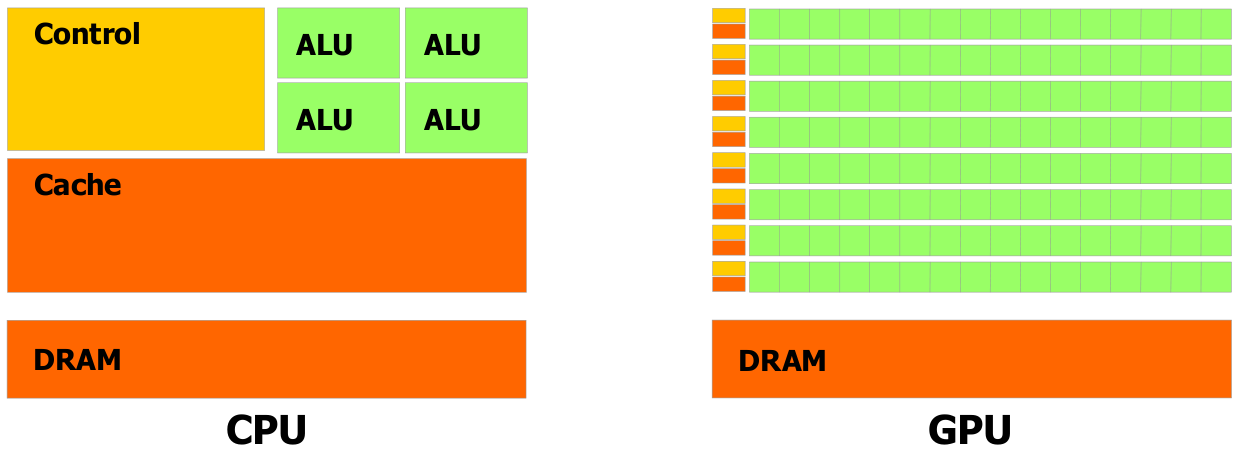
\includegraphics{CPUGPU.png}
\caption{This figure is from the \href{http://developer.download.nvidia.com/compute/DevZone/docs/html/C/doc/CUDA\_C\_Programming\_Guide.pdf}{NVIDIA CUDA Programming Guide}}\end{figure}

The graph above shows the differences between CPU and GPU in their structure. \textbf{Cache} is designed for data caching; \textbf{Control} is designed for flow control; \textbf{ALU} (Arithmetic Logic Unit) is designed for data processing.

In the NVISION 08 Conference organized by the NVIDIA corporation, employers from NVIDIA used a rather interesting yet straight forward example illustrating the difference between CPU and GPU. You can watch the video by clicking the link below and hope it can give you a better idea about what the difference between GPU and CPU is.
\href{http://www.NVIDIA.com/object/nvision08\_gpu\_v\_cpu.html}{Video}


\section{What is the advantage of using GPU for computation?}
\label{Introduction/Introduction:nvidia-cuda-programming-guide}\label{Introduction/Introduction:what-is-the-advantage-of-using-gpu-for-computation}
Nowadays, most of the scientific researches require massive data processing. What scientist usually do right now is to have all the data being processed on supercomputing clusters. Although most universities have constructed their own parallel computing clusters, researchers still need to compete for time to use the shared resources that not only cost millions to build and maintain, but also consume hundreds of kilowatts of power.

Different from traditional supercomputers that are built with many CPU cores, supercomputers with a GPU structure can achieve same level of performance with less cost and lower power consumption. \href{http://en.wikipedia.org/wiki/Nvidia\_Tesla\_\_Personal\_Supercomputer}{Personal Supercomputer} (PSC) based on NVIDIA's \href{http://www.nvidia.com/object/tesla-supercomputing-solutions.html}{Tesla} companion processors, was first introduced in 2008. The first generation four-GPU \href{http://www.nvidia.com/object/tesla-supercomputing-solutions.html}{Tesla} personal supercomputer have 4 Teraflops of parallel supercomputing performance, more than enough for most small researches. All it takes is 4 \href{http://www.nvidia.com/object/tesla-supercomputing-solutions.html}{Tesla} C1060 GPUs with 960 cores and two Intel Xeon processors. Moreover, Personal supercomputer is also very energy efficient as it can even run off a 110 volt wall circuit. Although supercomputer with GPUs cannot match the performance of the top ranking supercomputers that cost millions even billions, it is more than enough for researchers to perform daily research related computations in subjects like bioscience, life science, physics and geology.


\section{What are the important parts inside a GPU?}
\label{Introduction/Introduction:tesla}\label{Introduction/Introduction:what-are-the-important-parts-inside-a-gpu}
Although modern GPUs are basically computers themselves, they still serve as a part of a computer system. A modern GPU is connected with the host through a high speed I/O bus slot, usually a PCI-Express slot. Modern GPUs are extremely energy consuming. Some of the GPUs alone consume hundreds watts of power, sometimes higher than all other parts of the computer system combined. Part of the reason that GPUs require such power supply is that they have much complex  structure and can perform much sophisticated task than other parts of computer system. Owe to its high capability, GPU needs its own memory, control chipset as well as many processors.
\begin{figure}[htbp]
\centering
\capstart

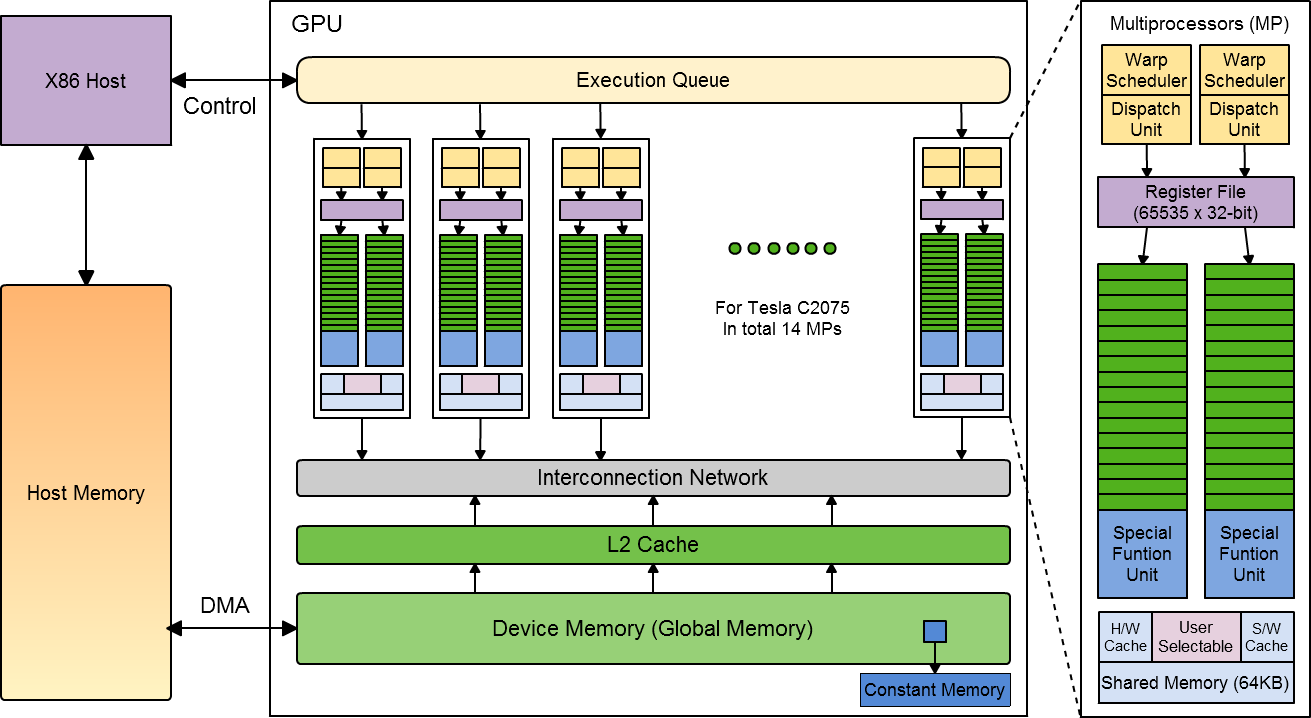
\includegraphics{CUDA.png}
\caption{This figure is inspired by the figure found in \href{http://www.pgroup.com/lit/articles/insider/v2n1a5.htm}{Understanding the CUDA Data Parallel Threading Model: A Primer} written by Michael Wolfe from The Portland Group}\end{figure}

GPUs these days are usually equipped with several gigabytes of on-board memory for user configuration. GPUs designed for daily use like gaming and video rendering, such as NVIDIA's \href{http://www.nvidia.com/object/geforce\_family.html}{Geforce} series GPUs and ATI/AMD's \href{http://www.amd.com/us/products/desktop/graphics/pages/desktop-graphics.aspx}{Radeon} series GPUs, have on-board memory capacity ranging from several hundreds megabytes to several gigabytes. Professional GPUs designed for high-definition image processing and General Purpose Computation, such as the \href{http://www.nvidia.com/object/tesla-supercomputing-solutions.html}{Tesla} Companion Processor we are using, usually have memory up to 5 or 6 gigabytes. Data are transferred between the GPU on-board memory and host memory through a method called DMA (Direct Memory Access). One thing worth mentioning is that CUDA C programming language supports direct access of the host memory from GPU end under certain restrictions. As GPU is designed for compute-intensive operations, device memory usually supports high data bandwidth with not deeply cached memory hierarchy.

GPUs from NVIDIA have many processors, called streaming Processors (SP). Each streaming processor is capable of executing a sequential thread. For a GPU with \emph{Fermi} architecture, like the one we are using, every 32 streaming processors is organized in a Streaming Multiprocessor (SM). A GPU can have one or more multiprocessors on board. For example, the \href{http://www.nvidia.com/object/tesla-supercomputing-solutions.html}{Tesla} C2075 GPU card we are using, has 14 multiprocessors built in. Except for 32 streaming processors, each multiprocessor is also equipped with 2 warp scheduler, 2 special function units (4 in some GPUs), a set of 32-bit registers and 64KB of configurable shared memory. A warp scheduler is responsible for threads control; SFU handles transcendentals and double-precision operations. For a GPU with \emph{Kepler} architecture, every 192 streaming processor is organized in a multiprocessor. There are also more warp schedulers and SFUs built in.

Shared memory, or L1 cache, is a small data cache that can be configured through software. Shared memory is also shared among all the streaming processors within one multiprocessor. Compared with on-board memory, shared memory is low-latency (usually register speed) and has high bandwidth. Each multiprocessor has 64KB of shared memory that can be configured by using special commands in host code. Shared memory is distributed to software-managed data cache and hardware data cache. The user can choose to assign either 48KB to software-managed data cache (SW) and 16KB to hardware data cache (HW) or the other way around.


\section{How does CUDA connect with hardware?}
\label{Introduction/Introduction:understanding-the-cuda-data-parallel-threading-model-a-primer}\label{Introduction/Introduction:how-does-cuda-connect-with-hardware}
When the host code invokes a kernel grid through a CUDA program, blocks in the grid are distributed to different multiprocessors based on available execution capacity of each multiprocessor. Each multiprocessor is capable of processing one or more blocks throughout the kernel execution. However, each block can only be processed by one multiprocessor.

Fermi architecture supports up to 48 active warps on each multiprocessor. The advantage of having many active warps in a process at the same time is significant reduction of memory latency. Traditionally, memory latency is reduced by adding more cache memory hierarchy into the system. However, by using high degree of multithreading, GPUs can also effectively reduce memory latency. What happens is that when one warp stalls on memory operation, the multiprocessor can select another warp and begin to process that one.

When a block is processed by a multiprocessor, threads in this block are further divided into groups of 32 threads, what NVIDIA calls a warp. Although 32 streaming processors in a block and 32 threads in a warp seems to be a good match for each multiprocessor to process each warp in one clock cycle, the reality is somehow different. As mentioned previously, each multiprocessor has two warp schedulers, which enables it to process two warps simultaneously. After the partition, each warp gets scheduled by a warp scheduler for execution. Each warp scheduler pumps 16 threads (half warp) into a group of 16 streaming processors for execution. Therefore, it would take two clock cycles to process each warp and one multiprocessor can process two warps in two clock cycles. For double-precision operations, each multiprocessor would combine two groups of streaming processors so that they act as a multiprocessor with 16 double-precision streaming processors.


\section{Is CUDA the only GPU programming language available?}
\label{Introduction/Introduction:is-cuda-the-only-gpu-programming-language-available}
When we are learning CUDA C programming language, it is important for you to know that the C programming language is not the only language that can be bound with CUDA structure. NVIDIA also made other programming languages available such as Fortran, Java and Python as binding languages with CUDA.

Furthermore, NVIDIA is not the only company manufacturing GPU cards, which means CUDA is not the only GPU programming MPI available. When NVIDIA were developing CUDA, AMD/ATI responded with \href{http://www.amd.com/stream/}{ATI Stream}, their GPGPU technology for AMD/ATI Radeon series GPUs. \href{http://www.amd.com/stream/}{ATI Stream} technology uses \href{http://en.wikipedia.org/wiki/OpenCL}{OpenCL} as its binding language.


\chapter{CUDA Intro}
\label{CUDAIntro/CUDAIntro:opencl}\label{CUDAIntro/CUDAIntro::doc}\label{CUDAIntro/CUDAIntro:cuda-intro}
Before we proceed to our first example, please follow the following instructions to set up your working environment.  The directory/folder structure needed for these examples is a folder called GPUProgramming with two folders inside of it, one called \emph{common} (from a tarball) and one called examples (you should make). Here's how to make them:
\begin{enumerate}
\item {} 
Create a top-level working folder for the code you will examine and run, called \code{GPUProgramming}.

\item {} 
Download the following file: \code{download common.tar.gz}

\item {} 
Extract all the files in \code{GPUProgramming}, which should create a folder \textbf{common}.

\item {} 
Create another folder called \code{examples} inside \code{GPUProgramming}. The examples folder will contain the CUDA code examples below.

\item {} 
Be sure to keep the common folder \textbf{outside} of your examples source code folder (this is because the example code includes code from ../common).

\end{enumerate}

\begin{notice}{note}{Note:}
Inside the common folder is the source code that contains helper functions. These include some error handling functions and APIs required for the later graphic programs, such as ray-tracing.
\end{notice}


\section{Acknowledgement}
\label{CUDAIntro/CUDAIntro:acknowledgement}
The examples used in this chapter are based on examples in \href{http://developer.nvidia.com/content/cuda-example-introduction-general-purpose-gpu-programming-0}{CUDA BY EXAMPLE: An Introduction to General-Purpose GPU Programming}, written by Jason Sanders and Edward Kandrot, and published by Addison Wesley.

Copyright 1993-2010 NVIDIA Corporation.  All rights reserved.

This copy of code is a derivative based on the original code and designed for educational purposes only. It contains source code provided by \href{http://www.nvidia.com}{NVIDIA Corporation}.


\section{An Example of Vector Addition}
\label{CUDAIntro/CUDAIntro:nvidia-corporation}\label{CUDAIntro/CUDAIntro:an-example-of-vector-addition}
We will start our CUDA journey by learning a very simple example, the vector addition example. It basically takes two vectors that have the same dimensions, adds them together and then returns the new vector back.

Vector Addition source file:
\code{VA-GPU-11.cu}

Get this source file and open it in an editor or terminal window so that you can follow along as sections of the code are explained here.


\subsection{The Device Code}
\label{CUDAIntro/CUDAIntro:the-device-code}
As you may have noticed in your background reading about CUDA programming, CUDA programs execute in two separate places. One is called the host (your CPU), another is called device (your GPU). In our example, the add() function executes on the device (our GPU) and the rest of the C program executes on our CPU.

\begin{Verbatim}[commandchars=\\\{\}]
\PYG{n}{\PYGZus{}\PYGZus{}global\PYGZus{}\PYGZus{}} \PYG{k+kt}{void} \PYG{n+nf}{add}\PYG{p}{(} \PYG{k+kt}{int} \PYG{o}{*}\PYG{n}{a}\PYG{p}{,} \PYG{k+kt}{int} \PYG{o}{*}\PYG{n}{b}\PYG{p}{,} \PYG{k+kt}{int} \PYG{o}{*}\PYG{n}{c} \PYG{p}{)} \PYG{p}{\PYGZob{}}    
    \PYG{k+kt}{int} \PYG{n}{tid} \PYG{o}{=} \PYG{l+m+mi}{0}\PYG{p}{;}
    \PYG{c+c1}{// loop over all the element in the vector}
    \PYG{k}{while} \PYG{p}{(}\PYG{n}{tid} \PYG{o}{\PYGZlt{}} \PYG{n}{N}\PYG{p}{)}\PYG{p}{\PYGZob{}}
        \PYG{n}{c}\PYG{p}{[}\PYG{n}{tid}\PYG{p}{]} \PYG{o}{=} \PYG{n}{a}\PYG{p}{[}\PYG{n}{tid}\PYG{p}{]} \PYG{o}{+} \PYG{n}{b}\PYG{p}{[}\PYG{n}{tid}\PYG{p}{]}\PYG{p}{;}
        \PYG{n}{tid} \PYG{o}{+}\PYG{o}{=} \PYG{l+m+mi}{1}\PYG{p}{;} \PYG{c+c1}{// we are using one thread in one block}
    \PYG{p}{\PYGZcb{}}
\PYG{p}{\PYGZcb{}}
\end{Verbatim}

As shown in the code block above, we need to add a \textbf{\_\_global\_\_} qualifier to the function name of the original C code in order to let function add() execute on a device.

You might notice that this code is much like standard C code except for the \textbf{\_\_global\_\_} qualifier. We are seeing this because this version of vector addition's device code is utilizing only one core of the GPU. We can see this from the line

\begin{Verbatim}[commandchars=\\\{\}]
        \PYG{n}{tid} \PYG{o}{+}\PYG{o}{=} \PYG{l+m+mi}{1}\PYG{p}{;} \PYG{c+c1}{// we are using one thread in one block}
\end{Verbatim}

where we only add 1 to the \emph{tid}. In the later examples, where we will be using more cores of the GPU, you will see differences between CUDA C programming language and Standard C programming language.


\subsection{The Host Code}
\label{CUDAIntro/CUDAIntro:the-host-code}\setbox0\vbox{
\begin{minipage}{0.95\linewidth}
\textbf{Before you proceed}

\medskip


Unlike the device code, the host code is more complicated and requires more explanation. We advise you to download the source file provided at the beginning of this page and have it open in a separate window. We divided the host code into several parts for the purpose of easier explanation. However, looking at the host code as a whole might be helpful, especially for CUDA programming, where host codes are usually highly organized and structured.
\end{minipage}}
\begin{center}\setlength{\fboxsep}{5pt}\shadowbox{\box0}\end{center}

\begin{Verbatim}[commandchars=\\\{\}]
\PYG{k+kt}{int} \PYG{n+nf}{main}\PYG{p}{(} \PYG{k+kt}{void} \PYG{p}{)} \PYG{p}{\PYGZob{}}

    \PYG{k+kt}{int} \PYG{o}{*}\PYG{n}{a}\PYG{p}{,} \PYG{o}{*}\PYG{n}{b}\PYG{p}{,} \PYG{o}{*}\PYG{n}{c}\PYG{p}{;}
    \PYG{k+kt}{int} \PYG{o}{*}\PYG{n}{dev\PYGZus{}a}\PYG{p}{,} \PYG{o}{*}\PYG{n}{dev\PYGZus{}b}\PYG{p}{,} \PYG{o}{*}\PYG{n}{dev\PYGZus{}c}\PYG{p}{;}

    \PYG{c+c1}{// allocate memory on the CPU}
    \PYG{n}{a} \PYG{o}{=} \PYG{p}{(}\PYG{k+kt}{int}\PYG{o}{*}\PYG{p}{)}\PYG{n}{malloc}\PYG{p}{(} \PYG{n}{N} \PYG{o}{*} \PYG{k}{sizeof}\PYG{p}{(}\PYG{k+kt}{int}\PYG{p}{)} \PYG{p}{)}\PYG{p}{;}
    \PYG{n}{b} \PYG{o}{=} \PYG{p}{(}\PYG{k+kt}{int}\PYG{o}{*}\PYG{p}{)}\PYG{n}{malloc}\PYG{p}{(} \PYG{n}{N} \PYG{o}{*} \PYG{k}{sizeof}\PYG{p}{(}\PYG{k+kt}{int}\PYG{p}{)} \PYG{p}{)}\PYG{p}{;}
    \PYG{n}{c} \PYG{o}{=} \PYG{p}{(}\PYG{k+kt}{int}\PYG{o}{*}\PYG{p}{)}\PYG{n}{malloc}\PYG{p}{(} \PYG{n}{N} \PYG{o}{*} \PYG{k}{sizeof}\PYG{p}{(}\PYG{k+kt}{int}\PYG{p}{)} \PYG{p}{)}\PYG{p}{;}

    \PYG{c+c1}{// fill arrays 'a' and 'b' on the CPU}
    \PYG{k}{for} \PYG{p}{(}\PYG{k+kt}{int} \PYG{n}{i}\PYG{o}{=}\PYG{l+m+mi}{0}\PYG{p}{;} \PYG{n}{i}\PYG{o}{\PYGZlt{}}\PYG{n}{N}\PYG{p}{;} \PYG{n}{i}\PYG{o}{+}\PYG{o}{+}\PYG{p}{)} \PYG{p}{\PYGZob{}}
        \PYG{n}{a}\PYG{p}{[}\PYG{n}{i}\PYG{p}{]} \PYG{o}{=} \PYG{o}{-}\PYG{n}{i}\PYG{p}{;}
        \PYG{n}{b}\PYG{p}{[}\PYG{n}{i}\PYG{p}{]} \PYG{o}{=} \PYG{n}{i} \PYG{o}{*} \PYG{n}{i}\PYG{p}{;}
    \PYG{p}{\PYGZcb{}}
\end{Verbatim}

As shown in the code block above, similar to standard C programming, we first need to declare pointers. Notice that we declared two sets of pointers, one set is used to store data on host memory, another is used to store data on the device memory.


\subsubsection{The Event API}
\label{CUDAIntro/CUDAIntro:the-event-api}
Before we go any further, we need to first learn ways of measuring performance in CUDA runtime. How do we measure performance? That is, how fast can the program run? To be more specific, we will try to time the program.

The tool we use to measure the time GPU spends on a task is the CUDA \href{http://developer.download.nvidia.com/compute/cuda/4\_2/rel/toolkit/docs/online/group\_\_CUDART\_\_MEMORY\_g48efa06b81cc031b2aa6fdc2e9930741.html\#g48efa06b81cc031b2aa6fdc2e9930741}{Event API}.

\begin{Verbatim}[commandchars=\\\{\}]
    \PYG{c+c1}{// define events in the field}
    \PYG{n}{cudaEvent\PYGZus{}t}     \PYG{n}{start}\PYG{p}{,} \PYG{n}{stop}\PYG{p}{;}
    \PYG{c+c1}{// create two events we need}
    \PYG{n}{HANDLE\PYGZus{}ERROR}\PYG{p}{(} \PYG{n}{cudaEventCreate}\PYG{p}{(} \PYG{o}{\PYGZam{}}\PYG{n}{start} \PYG{p}{)} \PYG{p}{)}\PYG{p}{;}
    \PYG{n}{HANDLE\PYGZus{}ERROR}\PYG{p}{(} \PYG{n}{cudaEventCreate}\PYG{p}{(} \PYG{o}{\PYGZam{}}\PYG{n}{stop} \PYG{p}{)} \PYG{p}{)}\PYG{p}{;}
    \PYG{c+c1}{// instruct the runtime to record the event start. }
    \PYG{n}{HANDLE\PYGZus{}ERROR}\PYG{p}{(} \PYG{n}{cudaEventRecord}\PYG{p}{(} \PYG{n}{start}\PYG{p}{,} \PYG{l+m+mi}{0} \PYG{p}{)} \PYG{p}{)}\PYG{p}{;}
\end{Verbatim}

The first step of using an event is declaring the event. In this example we declared two events, one called start, which will record the start event and another called stop, which will record the stop event. After declaring the events, we can use the command \href{http://developer.download.nvidia.com/compute/cuda/4\_2/rel/toolkit/docs/online/group\_\_CUDART\_\_EVENT\_ga324d5ce3fbf46899b15e5e42ff9cfa5.html\#ga324d5ce3fbf46899b15e5e42ff9cfa5}{cudaEventRecord()} to record an event. You can think of recording an event as initializing it. You may also notice that we pass this command a second argument (0 in this case). In our example this argument is actually useless. If you are really interested in this, however, you can read more about CUDA streams.

We can see that there is another function HANDLE\_ERROR() around each of the commands. For the moment, this function does not do anything but returning errors if CUDA commands run into any.
\setbox0\vbox{
\begin{minipage}{0.95\linewidth}
\textbf{Why would we use Event API?}

\medskip


If you are a C programming language veteran you may ask the question: why don't we use the the timing functions in standard C, such as \emph{clock()} or \emph{timeval} structure, to perform this task? This is a really good question.

The fundamental motivation of using \href{http://developer.download.nvidia.com/compute/cuda/4\_2/rel/toolkit/docs/online/group\_\_CUDART\_\_MEMORY\_g48efa06b81cc031b2aa6fdc2e9930741.html\#g48efa06b81cc031b2aa6fdc2e9930741}{Event API} instead of timing functions in standard C lies on the differences between CPU and GPU computation. To be more specific, GPU is a companion computation device, which means the CPU has to call GPU to do computations every time. However, when the GPU is doing a computation, the CPU does not wait for it to finish its task, instead the CPU will continue to execute the next line of code while GPU is still working on the previous call. This \emph{asynchronous} feature of the GPU computation structure leads to possible inaccuracy when measuring time using standard C timing functions. Therefore, \href{http://developer.download.nvidia.com/compute/cuda/4\_2/rel/toolkit/docs/online/group\_\_CUDART\_\_MEMORY\_g48efa06b81cc031b2aa6fdc2e9930741.html\#g48efa06b81cc031b2aa6fdc2e9930741}{Event API} becomes needed.
\end{minipage}}
\begin{center}\setlength{\fboxsep}{5pt}\shadowbox{\box0}\end{center}


\subsubsection{The cudaMalloc() Function}
\label{CUDAIntro/CUDAIntro:the-cudamalloc-function}
\begin{Verbatim}[commandchars=\\\{\}]
    \PYG{c+c1}{// allocate memory on the GPU}
    \PYG{n}{HANDLE\PYGZus{}ERROR}\PYG{p}{(} \PYG{n}{cudaMalloc}\PYG{p}{(} \PYG{p}{(}\PYG{k+kt}{void}\PYG{o}{*}\PYG{o}{*}\PYG{p}{)}\PYG{o}{\PYGZam{}}\PYG{n}{dev\PYGZus{}a}\PYG{p}{,} \PYG{n}{N} \PYG{o}{*} \PYG{k}{sizeof}\PYG{p}{(}\PYG{k+kt}{int}\PYG{p}{)} \PYG{p}{)} \PYG{p}{)}\PYG{p}{;}
    \PYG{n}{HANDLE\PYGZus{}ERROR}\PYG{p}{(} \PYG{n}{cudaMalloc}\PYG{p}{(} \PYG{p}{(}\PYG{k+kt}{void}\PYG{o}{*}\PYG{o}{*}\PYG{p}{)}\PYG{o}{\PYGZam{}}\PYG{n}{dev\PYGZus{}b}\PYG{p}{,} \PYG{n}{N} \PYG{o}{*} \PYG{k}{sizeof}\PYG{p}{(}\PYG{k+kt}{int}\PYG{p}{)} \PYG{p}{)} \PYG{p}{)}\PYG{p}{;}
    \PYG{n}{HANDLE\PYGZus{}ERROR}\PYG{p}{(} \PYG{n}{cudaMalloc}\PYG{p}{(} \PYG{p}{(}\PYG{k+kt}{void}\PYG{o}{*}\PYG{o}{*}\PYG{p}{)}\PYG{o}{\PYGZam{}}\PYG{n}{dev\PYGZus{}c}\PYG{p}{,} \PYG{n}{N} \PYG{o}{*} \PYG{k}{sizeof}\PYG{p}{(}\PYG{k+kt}{int}\PYG{p}{)} \PYG{p}{)} \PYG{p}{)}\PYG{p}{;}
\end{Verbatim}

Just like the standard C programming language, you need to allocate memory for variables before you start using them. The command \href{http://developer.download.nvidia.com/compute/cuda/4\_2/rel/toolkit/docs/online/group\_\_CUDART\_\_MEMORY\_gc63ffd93e344b939d6399199d8b12fef.html\#gc63ffd93e344b939d6399199d8b12fef}{cudaMalloc()}, similar to \emph{malloc()} command in standard C, tells the CUDA runtime to allocate memory on the device (Memory of GPU), instead of on the host (Memory of CPU). The first argument is a pointer that points to where you want to hold the address of the newly allocated memory.

Because the memory units on the host are separate from those on the GPU, you are not allowed to modify memory allocated on the device (GPU) from the host directly in CUDA C programming language. Instead, you need to use two other methods to access the device memory. You can do it by either using device pointers in the device code, or you can use the \href{http://developer.download.nvidia.com/compute/cuda/4\_2/rel/toolkit/docs/online/group\_\_CUDART\_\_MEMORY\_g48efa06b81cc031b2aa6fdc2e9930741.html\#g48efa06b81cc031b2aa6fdc2e9930741}{cudaMemcpy()} method.

The way to use pointers in the device code is exactly the same as we did in the host code. In other words, a pointer in CUDA C is exactly the same as in standard C. However, there is one thing you need to pay attention to. Host pointers can only access memory (usually CPU memory) from host code, you cannot access device memory directly. On the other hand, device pointers can only access GPU memory from device code as well.


\subsubsection{The cudaMemcpy() Function}
\label{CUDAIntro/CUDAIntro:the-cudamemcpy-function}
\begin{Verbatim}[commandchars=\\\{\}]
    \PYG{c+c1}{// copy arrays 'a' and 'b' to the GPU}
    \PYG{n}{HANDLE\PYGZus{}ERROR}\PYG{p}{(} \PYG{n}{cudaMemcpy}\PYG{p}{(} \PYG{n}{dev\PYGZus{}a}\PYG{p}{,} \PYG{n}{a}\PYG{p}{,} \PYG{n}{N} \PYG{o}{*} \PYG{k}{sizeof}\PYG{p}{(}\PYG{k+kt}{int}\PYG{p}{)}\PYG{p}{,}
                              \PYG{n}{cudaMemcpyHostToDevice} \PYG{p}{)} \PYG{p}{)}\PYG{p}{;}
    \PYG{n}{HANDLE\PYGZus{}ERROR}\PYG{p}{(} \PYG{n}{cudaMemcpy}\PYG{p}{(} \PYG{n}{dev\PYGZus{}b}\PYG{p}{,} \PYG{n}{b}\PYG{p}{,} \PYG{n}{N} \PYG{o}{*} \PYG{k}{sizeof}\PYG{p}{(}\PYG{k+kt}{int}\PYG{p}{)}\PYG{p}{,}
                              \PYG{n}{cudaMemcpyHostToDevice} \PYG{p}{)} \PYG{p}{)}\PYG{p}{;}
\end{Verbatim}

As mentioned in the last section, we can use \href{http://developer.download.nvidia.com/compute/cuda/4\_2/rel/toolkit/docs/online/group\_\_CUDART\_\_MEMORY\_g48efa06b81cc031b2aa6fdc2e9930741.html\#g48efa06b81cc031b2aa6fdc2e9930741}{cudaMemcpy()} from host code to place data in memory on a device. \textbf{This command is the typical way of transferring data between host and device.} This call is similar to the standard C call \emph{memcpy()}, but requires more parameters. The first argument identifies the destination pointer; the second identifies the source pointer. The last parameter to the call is \href{http://developer.download.nvidia.com/compute/cuda/4\_2/rel/toolkit/docs/online/group\_\_CUDART\_\_TYPES\_g18fa99055ee694244a270e4d5101e95b.html\#gg18fa99055ee694244a270e4d5101e95b1a03d03a676ea8ec51b9b1e193617568}{cudaMemcpyHostToDevice}, telling the runtime that the source pointer is a host pointer and the destination pointer is a device pointer.


\subsubsection{The Kernel Invocation}
\label{CUDAIntro/CUDAIntro:the-kernel-invocation}
The following line in main() is the call for device code to be executed, in this case the function add(), which was shown earlier. You may notice that this call is similar to a normal function call but has additional code in it, notably the \textless{}\textless{}\textless{} , the \textgreater{}\textgreater{}\textgreater{}, and what lies in between them (the triple angle brackets). We will talk about what they represent in later examples. At this point all you need to know is that they are telling the GPU to use only one thread to execute the program.

\begin{Verbatim}[commandchars=\\\{\}]
    \PYG{c+c1}{// kernel invocation code}
    \PYG{n}{add}\PYG{o}{\PYGZlt{}}\PYG{o}{\PYGZlt{}}\PYG{o}{\PYGZlt{}}\PYG{l+m+mi}{1}\PYG{p}{,}\PYG{l+m+mi}{1}\PYG{o}{\PYGZgt{}}\PYG{o}{\PYGZgt{}}\PYG{o}{\PYGZgt{}}\PYG{p}{(} \PYG{n}{dev\PYGZus{}a}\PYG{p}{,} \PYG{n}{dev\PYGZus{}b}\PYG{p}{,} \PYG{n}{dev\PYGZus{}c} \PYG{p}{)}\PYG{p}{;}
\end{Verbatim}


\subsubsection{More cudaMemcpy() Function}
\label{CUDAIntro/CUDAIntro:more-cudamemcpy-function}
\begin{Verbatim}[commandchars=\\\{\}]
    \PYG{c+c1}{// copy array 'c' back from the GPU to the CPU}
    \PYG{n}{HANDLE\PYGZus{}ERROR}\PYG{p}{(} \PYG{n}{cudaMemcpy}\PYG{p}{(} \PYG{n}{c}\PYG{p}{,} \PYG{n}{dev\PYGZus{}c}\PYG{p}{,} \PYG{n}{N} \PYG{o}{*} \PYG{k}{sizeof}\PYG{p}{(}\PYG{k+kt}{int}\PYG{p}{)}\PYG{p}{,}
                              \PYG{n}{cudaMemcpyDeviceToHost} \PYG{p}{)} \PYG{p}{)}\PYG{p}{;}
\end{Verbatim}

In the previous section we have seen how CUDA runtime transfers data from Host to Device. This time we will see how to transfer data back to the host. Notice that this time device memory is the source and host memory is the destination. Therefore, we are using the argument \href{http://developer.download.nvidia.com/compute/cuda/4\_2/rel/toolkit/docs/online/group\_\_CUDART\_\_TYPES\_g18fa99055ee694244a270e4d5101e95b.html\#gg18fa99055ee694244a270e4d5101e95b1a03d03a676ea8ec51b9b1e193617568}{cudaMemcpyDeviceToHost}.


\subsubsection{Timing using Event API}
\label{CUDAIntro/CUDAIntro:timing-using-event-api}
\begin{Verbatim}[commandchars=\\\{\}]
    \PYG{c+c1}{// get stop time, and display the timing results}
    \PYG{n}{HANDLE\PYGZus{}ERROR}\PYG{p}{(} \PYG{n}{cudaEventRecord}\PYG{p}{(} \PYG{n}{stop}\PYG{p}{,} \PYG{l+m+mi}{0} \PYG{p}{)} \PYG{p}{)}\PYG{p}{;}
    \PYG{n}{HANDLE\PYGZus{}ERROR}\PYG{p}{(} \PYG{n}{cudaEventSynchronize}\PYG{p}{(} \PYG{n}{stop} \PYG{p}{)} \PYG{p}{)}\PYG{p}{;}
    \PYG{k+kt}{float}   \PYG{n}{elapsedTime}\PYG{p}{;}
    \PYG{n}{HANDLE\PYGZus{}ERROR}\PYG{p}{(} \PYG{n}{cudaEventElapsedTime}\PYG{p}{(} \PYG{o}{\PYGZam{}}\PYG{n}{elapsedTime}\PYG{p}{,}
                                        \PYG{n}{start}\PYG{p}{,} \PYG{n}{stop} \PYG{p}{)} \PYG{p}{)}\PYG{p}{;}
    \PYG{n}{printf}\PYG{p}{(} \PYG{l+s}{"}\PYG{l+s}{Time to generate:  \PYGZpc{}3.1f ms}\PYG{l+s+se}{\PYGZbs{}n}\PYG{l+s}{"}\PYG{p}{,} \PYG{n}{elapsedTime} \PYG{p}{)}\PYG{p}{;}
\end{Verbatim}

We have seen how to declare and record an \href{http://developer.download.nvidia.com/compute/cuda/4\_2/rel/toolkit/docs/online/group\_\_CUDART\_\_MEMORY\_g48efa06b81cc031b2aa6fdc2e9930741.html\#g48efa06b81cc031b2aa6fdc2e9930741}{Event API} in CUDA C, but have not elaborated on how to use such a tool to measure performance. The basic idea is that we first declare an event start and an event stop. Then at the beginning of the program we record event start and at the end of the program we record event stop. The last step is to calculate the elapsed time between two events.

As shown in the code block above, we again use the command \href{http://developer.download.nvidia.com/compute/cuda/4\_2/rel/toolkit/docs/online/group\_\_CUDART\_\_EVENT\_ga324d5ce3fbf46899b15e5e42ff9cfa5.html\#ga324d5ce3fbf46899b15e5e42ff9cfa5}{cudaEventRecord()} to instruct the runtime to record the event stop. Then we proceed to the last step, which is to get the elapsed time using the command \href{http://developer.download.nvidia.com/compute/cuda/4\_2/rel/toolkit/docs/online/group\_\_CUDART\_\_EVENT\_g14c387cc57ce2e328f6669854e6020a5.html\#g14c387cc57ce2e328f6669854e6020a5}{cudaEventElapsedTime()}.

However, there is still a problem with timing GPU code in this way. Though the CUDA C programming language though is derived from standard C, it has many characteristics that are different from standard C. We have mentioned in previous sections that CUDA C is asynchronous. This is an example to jog your memory. Suppose we are running a program to do matrix multiplication, and the host calls the GPU to do the computation. As GPU begins executing our code, the CPU proceeds to the next line of code instead of waiting for the GPU to finish its work. If we want the stop the event to record the correct time, we need to make sure that our event is recorded after the GPU finishes everything prior to the call to \href{http://developer.download.nvidia.com/compute/cuda/4\_2/rel/toolkit/docs/online/group\_\_CUDART\_\_EVENT\_ga324d5ce3fbf46899b15e5e42ff9cfa5.html\#ga324d5ce3fbf46899b15e5e42ff9cfa5}{cudaEventRecord()}. To address this problem, CUDA C calls the function \href{http://developer.download.nvidia.com/compute/cuda/4\_2/rel/toolkit/docs/online/group\_\_CUDART\_\_EVENT\_g08241bcf5c5cb686b1882a8492f1e2d9.html\#g08241bcf5c5cb686b1882a8492f1e2d9}{cudaEventSynchronize()} to synchronize the stop event.

The \href{http://developer.download.nvidia.com/compute/cuda/4\_2/rel/toolkit/docs/online/group\_\_CUDART\_\_EVENT\_g08241bcf5c5cb686b1882a8492f1e2d9.html\#g08241bcf5c5cb686b1882a8492f1e2d9}{cudaEventSynchronize()} function is essentially instructing the runtime to create a barrier to block the CPU from executing further instructions until the GPU has reached the stop event.

Another caveat worth mentioning is that CUDA events are implemented directly on the GPU. Therefore they cannot be used for timing device code mixed with host code. In other words, you will get unreliable results if you attempt to use CUDA events to time more than kernel executions and memory copies involving the device.

\begin{notice}{note}{Note:}
You should only include kernel execution and memory copies involving the device in between start event and stop event in CUDA. Anything more included could lead to unreliable results.
\end{notice}


\subsubsection{The cudaFree() Function}
\label{CUDAIntro/CUDAIntro:the-cudafree-function}
\begin{Verbatim}[commandchars=\\\{\}]
    \PYG{c+c1}{// free memory allocated on the GPU}
    \PYG{n}{HANDLE\PYGZus{}ERROR}\PYG{p}{(} \PYG{n}{cudaFree}\PYG{p}{(} \PYG{n}{dev\PYGZus{}a} \PYG{p}{)} \PYG{p}{)}\PYG{p}{;}
    \PYG{n}{HANDLE\PYGZus{}ERROR}\PYG{p}{(} \PYG{n}{cudaFree}\PYG{p}{(} \PYG{n}{dev\PYGZus{}b} \PYG{p}{)} \PYG{p}{)}\PYG{p}{;}
    \PYG{n}{HANDLE\PYGZus{}ERROR}\PYG{p}{(} \PYG{n}{cudaFree}\PYG{p}{(} \PYG{n}{dev\PYGZus{}c} \PYG{p}{)} \PYG{p}{)}\PYG{p}{;}

    \PYG{c+c1}{// destroy events to free memory}
    \PYG{n}{HANDLE\PYGZus{}ERROR}\PYG{p}{(} \PYG{n}{cudaEventDestroy}\PYG{p}{(} \PYG{n}{start} \PYG{p}{)} \PYG{p}{)}\PYG{p}{;}
    \PYG{n}{HANDLE\PYGZus{}ERROR}\PYG{p}{(} \PYG{n}{cudaEventDestroy}\PYG{p}{(} \PYG{n}{stop} \PYG{p}{)} \PYG{p}{)}\PYG{p}{;}
\end{Verbatim}

While reading the section about \href{http://developer.download.nvidia.com/compute/cuda/4\_2/rel/toolkit/docs/online/group\_\_CUDART\_\_MEMORY\_gc63ffd93e344b939d6399199d8b12fef.html\#gc63ffd93e344b939d6399199d8b12fef}{cudaMalloc()}, it may occur to you that we made a call different from the call \emph{free()} to free memory on the device. To free memory allocated on the device, we need to use command \href{http://developer.download.nvidia.com/compute/cuda/4\_2/rel/toolkit/docs/online/group\_\_CUDART\_\_MEMORY\_gb17fef862d4d1fefb9dba35bd62a187e.html\#gb17fef862d4d1fefb9dba35bd62a187e}{cudaFree()} instead of free().

To finish up the code, we need to free memory allocated on the CPU as well.

\begin{Verbatim}[commandchars=\\\{\}]
    \PYG{c+c1}{// free memory allocated on the CPU}
    \PYG{n}{free}\PYG{p}{(} \PYG{n}{a} \PYG{p}{)}\PYG{p}{;}
    \PYG{n}{free}\PYG{p}{(} \PYG{n}{b} \PYG{p}{)}\PYG{p}{;}
    \PYG{n}{free}\PYG{p}{(} \PYG{n}{c} \PYG{p}{)}\PYG{p}{;}
\end{Verbatim}

The following code is useful to verify whether the GPU has done the task correctly or not. This time we are using CPU to verify GPU's work. We can do this in this problem due to a small data size and simple computation.

\begin{Verbatim}[commandchars=\\\{\}]
    \PYG{n}{bool} \PYG{n}{success} \PYG{o}{=} \PYG{n+nb}{true}\PYG{p}{;}
    \PYG{k}{for} \PYG{p}{(}\PYG{k+kt}{int} \PYG{n}{i}\PYG{o}{=}\PYG{l+m+mi}{0}\PYG{p}{;} \PYG{n}{i}\PYG{o}{\PYGZlt{}}\PYG{n}{N}\PYG{p}{;} \PYG{n}{i}\PYG{o}{+}\PYG{o}{+}\PYG{p}{)} \PYG{p}{\PYGZob{}}
        \PYG{k}{if} \PYG{p}{(}\PYG{p}{(}\PYG{n}{a}\PYG{p}{[}\PYG{n}{i}\PYG{p}{]} \PYG{o}{+} \PYG{n}{b}\PYG{p}{[}\PYG{n}{i}\PYG{p}{]}\PYG{p}{)} \PYG{o}{!}\PYG{o}{=} \PYG{n}{c}\PYG{p}{[}\PYG{n}{i}\PYG{p}{]}\PYG{p}{)} \PYG{p}{\PYGZob{}}
            \PYG{n}{printf}\PYG{p}{(} \PYG{l+s}{"}\PYG{l+s}{Error:  \PYGZpc{}d + \PYGZpc{}d != \PYGZpc{}d}\PYG{l+s+se}{\PYGZbs{}n}\PYG{l+s}{"}\PYG{p}{,} \PYG{n}{a}\PYG{p}{[}\PYG{n}{i}\PYG{p}{]}\PYG{p}{,} \PYG{n}{b}\PYG{p}{[}\PYG{n}{i}\PYG{p}{]}\PYG{p}{,} \PYG{n}{c}\PYG{p}{[}\PYG{n}{i}\PYG{p}{]} \PYG{p}{)}\PYG{p}{;}
            \PYG{n}{success} \PYG{o}{=} \PYG{n+nb}{false}\PYG{p}{;}
        \PYG{p}{\PYGZcb{}}
    \PYG{p}{\PYGZcb{}}
    \PYG{k}{if} \PYG{p}{(}\PYG{n}{success}\PYG{p}{)}  \PYG{n}{printf}\PYG{p}{(} \PYG{l+s}{"}\PYG{l+s}{We did it!}\PYG{l+s+se}{\PYGZbs{}n}\PYG{l+s}{"} \PYG{p}{)}\PYG{p}{;}
\end{Verbatim}


\subsection{Compiling the code and executing this example}
\label{CUDAIntro/CUDAIntro:compiling-the-code-and-executing-this-example}
From the \emph{examples} folder where your file VA-GPU-11.cu is located, you compile the code using the \textbf{nvcc} compiler.  On unix machines we do this on the command line like this:

\begin{Verbatim}[commandchars=\\\{\}]
nvcc -o VA-GPU-11 VA-GPU-11.cu
\end{Verbatim}

Run the executable called \emph{VA-GPU-11}.  On unix machines we do this on the command line like this:

\begin{Verbatim}[commandchars=\\\{\}]
./VA-GPU-11
\end{Verbatim}

This example is only using one thread on the GPU card, so it is not yet a parallel programming example.  Furthermore, you would never go to the trouble of moving data just to use one of the many cores available on the GPU card! Continue on to see how we take advantage of those cores.

\begin{notice}{note}{Note:}
Before moving on, execute this code a few times and record how much time it takes on your CUDA-enabled GOU.
\end{notice}


\bigskip\hrule{}\bigskip



\section{Vector Addition with Blocks}
\label{CUDAIntro/CUDAIntro:vector-addition-with-blocks}\label{CUDAIntro/CUDAIntro:cudamemcpydevicetohost}
We have learned some basic concepts in CUDA C in our last example. Starting from this next example, we will begin to learn how to write CUDA language that will explore the potential of our GPU card.

Download this Vector Addition with Blocks source file:
\code{VA-GPU-N1.cu}  into the examples directory where you placed the previous example code file.


\subsection{Block}
\label{CUDAIntro/CUDAIntro:block}
Recall that in the previous example, we used the code

\begin{Verbatim}[commandchars=\\\{\}]
    \PYG{n}{add}\PYG{o}{\PYGZlt{}}\PYG{o}{\PYGZlt{}}\PYG{o}{\PYGZlt{}}\PYG{l+m+mi}{1}\PYG{p}{,}\PYG{l+m+mi}{1}\PYG{o}{\PYGZgt{}}\PYG{o}{\PYGZgt{}}\PYG{o}{\PYGZgt{}}\PYG{p}{(} \PYG{n}{dev\PYGZus{}a}\PYG{p}{,} \PYG{n}{dev\PYGZus{}b}\PYG{p}{,} \PYG{n}{dev\PYGZus{}c} \PYG{p}{)}\PYG{p}{;}
\end{Verbatim}

to run device `kernel' code and we left those two numbers in the triple angle brackets unexplained. Well, the first number tells the kernel how many parallel blocks we would like to use to execute the function. For example, if we launch the kernel function with \textless{}\textless{}\textless{}16,1\textgreater{}\textgreater{}\textgreater{}, we are essentially creating 16 copies of the kernel function and running them in parallel.  CUDA developers call each of these parallel invocations a \emph{block}.

Blocks are organized into a one-dimensional, two-dimensional, or three-dimensional grid. Why do we need a two-dimensional or even a three-dimensional grid? Why can't we just stick with the one-dimensional grid? Well, it turns out that for problems with two or more dimensional domains, such as matrix multiplication or image processing (don't forget the reason GPU been exist is to process images faster), it is often convenient and more efficient to use two or more dimensional indexing. Right now, nVidia GPUs that support CUDA structure can assign up to 65536 blocks in each dimension of the grid, that is in total $65536 \times 65536 \times 65536$ blocks in a grid.

\begin{notice}{note}{Note:}
Some books imply that the grid in CUDA has at most two-dimensions. On the other hand, some books (including the official CUDA Programming Guide provided by NVIDIA) suggest that the grid can be three-dimensional. It turns out that older GPU units are not powerful enough to run grids in three-dimensions. Therefore older books might argue that CUDA has only a two-dimensional grid. However, as GPUs get more and more powerful, NVIDIA enable newer GPUs to utilize three-dimensional grids.

To see whether your device supports three-dimensional grids or not, please run the following source code and see the Compute Capability entry in the output. If it is 2.x or 3.x, then your device supports three-dimensional grids. If it is 1.x or less, you can only use two-dimensional grids. \code{download enum\_gpu.cu}
\end{notice}


\subsection{The Device Code}
\label{CUDAIntro/CUDAIntro:id1}
\begin{Verbatim}[commandchars=\\\{\}]
\PYG{n}{\PYGZus{}\PYGZus{}global\PYGZus{}\PYGZus{}} \PYG{k+kt}{void} \PYG{n+nf}{add}\PYG{p}{(} \PYG{k+kt}{int} \PYG{o}{*}\PYG{n}{a}\PYG{p}{,} \PYG{k+kt}{int} \PYG{o}{*}\PYG{n}{b}\PYG{p}{,} \PYG{k+kt}{int} \PYG{o}{*}\PYG{n}{c} \PYG{p}{)} \PYG{p}{\PYGZob{}}

    \PYG{c+c1}{// keep track of the index}
    \PYG{k+kt}{int} \PYG{n}{tid} \PYG{o}{=} \PYG{n}{blockIdx}\PYG{p}{.}\PYG{n}{x}\PYG{p}{;}

    \PYG{k}{while} \PYG{p}{(}\PYG{n}{tid} \PYG{o}{\PYGZlt{}} \PYG{n}{N}\PYG{p}{)} \PYG{p}{\PYGZob{}}
        \PYG{n}{c}\PYG{p}{[}\PYG{n}{tid}\PYG{p}{]} \PYG{o}{=} \PYG{n}{a}\PYG{p}{[}\PYG{n}{tid}\PYG{p}{]} \PYG{o}{+} \PYG{n}{b}\PYG{p}{[}\PYG{n}{tid}\PYG{p}{]}\PYG{p}{;}
        \PYG{n}{tid} \PYG{o}{+}\PYG{o}{=} \PYG{n}{numBlock}\PYG{p}{;} \PYG{c+c1}{// shift by the total number of blocks}
    \PYG{p}{\PYGZcb{}}
\PYG{p}{\PYGZcb{}}
\end{Verbatim}

This is the complete device code.

We have mentioned that there are one, two and three-dimensional grids. To index different blocks in a grid, we use the built-in variables CUDA runtime defines for us: blockIdx. The variable blockIdx is a three-component vector, so that threads can be identified using a one-dimensional, two-dimensional or three-dimensional index. To access different components in this vector, we use blockIdx.x, blockIdx.y and blockIdx.z.

\begin{Verbatim}[commandchars=\\\{\}]
    \PYG{c+c1}{// keep track of the index}
    \PYG{k+kt}{int} \PYG{n}{tid} \PYG{o}{=} \PYG{n}{blockIdx}\PYG{p}{.}\PYG{n}{x}\PYG{p}{;}
\end{Verbatim}

Since we have multiple blocks performing the same task, we need to keep track of these blocks so that the kernel can pass the right data to them and bring the right data back. Since we have only 1 thread in each block, we can simply use blockIdx to track the index.

\begin{Verbatim}[commandchars=\\\{\}]
        \PYG{n}{tid} \PYG{o}{+}\PYG{o}{=} \PYG{n}{numBlock}\PYG{p}{;} \PYG{c+c1}{// shift by the total number of blocks}
\end{Verbatim}

Although we have multiple blocks (1 thread per block) working simultaneously after one block finishes one computation, this does not necessarily mean a block will only perform one time of computation. Normally, we could have a problem size that is larger than the number of blocks we have. Therefore, we need each block to perform more than one time of computation. We do this by adding a stride to the tid after the while loop finishes one round. In this example, we want tid to shift to the next data point by the total number of blocks.


\subsection{The Host Code}
\label{CUDAIntro/CUDAIntro:id2}
\begin{Verbatim}[commandchars=\\\{\}]
    \PYG{n}{add}\PYG{o}{\PYGZlt{}}\PYG{o}{\PYGZlt{}}\PYG{o}{\PYGZlt{}}\PYG{n}{numBlock}\PYG{p}{,}\PYG{n}{numThread}\PYG{o}{\PYGZgt{}}\PYG{o}{\PYGZgt{}}\PYG{o}{\PYGZgt{}}\PYG{p}{(} \PYG{n}{dev\PYGZus{}a}\PYG{p}{,} \PYG{n}{dev\PYGZus{}b}\PYG{p}{,} \PYG{n}{dev\PYGZus{}c} \PYG{p}{)}\PYG{p}{;}
\end{Verbatim}

Except the kernel invocation part of the host code, everything else is the same. However, as we are calling \textbf{numBlock} and \textbf{numThread} in the code, we need to define them at the very beginning of the source code file.

\begin{Verbatim}[commandchars=\\\{\}]
\PYG{c+cp}{\PYGZsh{}}\PYG{c+cp}{define numThread 1 }\PYG{c+c1}{// in this example we keep one thread in one block}
\PYG{c+cp}{\PYGZsh{}}\PYG{c+cp}{define numBlock 128 }\PYG{c+c1}{// in this example we use multiple blocks}
\end{Verbatim}


\bigskip\hrule{}\bigskip



\section{Vector Addition with Blocks and Threads}
\label{CUDAIntro/CUDAIntro:vector-addition-with-blocks-and-threads}
Vector Addition with Blocks and Threads source file:
\code{VA-GPU-NN.cu}


\subsection{Threads}
\label{CUDAIntro/CUDAIntro:threads}
In the last example we learned how to launch multiple blocks in CUDA C programs. This time, we will see how to split parallel blocks. CUDA runtime allows us to split blocks into threads. Recall that in the previous example we use the code

\begin{Verbatim}[commandchars=\\\{\}]
    \PYG{n}{add}\PYG{o}{\PYGZlt{}}\PYG{o}{\PYGZlt{}}\PYG{o}{\PYGZlt{}}\PYG{n}{numBlock}\PYG{p}{,}\PYG{n}{numThread}\PYG{o}{\PYGZgt{}}\PYG{o}{\PYGZgt{}}\PYG{o}{\PYGZgt{}}\PYG{p}{(} \PYG{n}{dev\PYGZus{}a}\PYG{p}{,} \PYG{n}{dev\PYGZus{}b}\PYG{p}{,} \PYG{n}{dev\PYGZus{}c} \PYG{p}{)}\PYG{p}{;}
\end{Verbatim}

to call for device kernels where numBlock is 128 and numThread remain as 1. The second number represents how many threads we want in each block.

Here comes the question, why do we need two sets of parallel organization system? Why do we need not only blocks in grid, but also threads in blocks? Are there any advantages in one over the other? Well, there are advantages that we will cover in later examples, so for now, please bear with us.

Just like blocks are organized in up to three-dimensional grids, threads can also be organized in one, two or three-dimensional blocks. Just like there is a limit on the number of blocks in a grid, there is also a limit on the number of threads in a block. Right now, for most of the high-end nVidia GPUs, this limit is 1024. Be really careful here, 1024 is the total number of threads in a block, \textbf{not} the limit \textbf{per dimension} like in the grid. Most of the nVidia GPUs that are two or three year old, the limit might be 512. You can query the maxThreadsPerBlock field of the device properties structure to find out which number you have.


\subsection{The Device Code}
\label{CUDAIntro/CUDAIntro:id3}
\begin{Verbatim}[commandchars=\\\{\}]
\PYG{n}{\PYGZus{}\PYGZus{}global\PYGZus{}\PYGZus{}} \PYG{k+kt}{void} \PYG{n+nf}{add}\PYG{p}{(} \PYG{k+kt}{int} \PYG{o}{*}\PYG{n}{a}\PYG{p}{,} \PYG{k+kt}{int} \PYG{o}{*}\PYG{n}{b}\PYG{p}{,} \PYG{k+kt}{int} \PYG{o}{*}\PYG{n}{c} \PYG{p}{)} \PYG{p}{\PYGZob{}}

    \PYG{c+c1}{// keep track of the index}
    \PYG{k+kt}{int} \PYG{n}{tid} \PYG{o}{=} \PYG{n}{threadIdx}\PYG{p}{.}\PYG{n}{x} \PYG{o}{+} \PYG{n}{blockIdx}\PYG{p}{.}\PYG{n}{x} \PYG{o}{*} \PYG{n}{numBlock}\PYG{p}{;}

    \PYG{k}{while} \PYG{p}{(}\PYG{n}{tid} \PYG{o}{\PYGZlt{}} \PYG{n}{N}\PYG{p}{)} \PYG{p}{\PYGZob{}}
        \PYG{n}{c}\PYG{p}{[}\PYG{n}{tid}\PYG{p}{]} \PYG{o}{=} \PYG{n}{a}\PYG{p}{[}\PYG{n}{tid}\PYG{p}{]} \PYG{o}{+} \PYG{n}{b}\PYG{p}{[}\PYG{n}{tid}\PYG{p}{]}\PYG{p}{;}
        \PYG{n}{tid} \PYG{o}{+}\PYG{o}{=} \PYG{n}{numThread} \PYG{o}{*} \PYG{n}{numBlock}\PYG{p}{;}\PYG{c+c1}{// shift by the total number of thread in a grid}
    \PYG{p}{\PYGZcb{}}
\PYG{p}{\PYGZcb{}}
\end{Verbatim}

This is the complete device code.

Just like we use CUDA built-in variables to index blocks in a grid, we use variable threadIdx to index threads in a block. threadIdx is also a three-component vector and you can access each of its element using threadIdx.x, threadIdx,y and threadIdx.z.

\begin{Verbatim}[commandchars=\\\{\}]
    \PYG{c+c1}{// keep track of the index}
    \PYG{k+kt}{int} \PYG{n}{tid} \PYG{o}{=} \PYG{n}{threadIdx}\PYG{p}{.}\PYG{n}{x} \PYG{o}{+} \PYG{n}{blockIdx}\PYG{p}{.}\PYG{n}{x} \PYG{o}{*} \PYG{n}{numBlock}\PYG{p}{;}
\end{Verbatim}

The thread handles the data at its thread id. Recall that earlier we were using tid = blockIdx.x only. Now, as we are using multiple threads per block, we have to keep track of not only blockId, but also the threadId as well.

\begin{Verbatim}[commandchars=\\\{\}]
        \PYG{n}{tid} \PYG{o}{+}\PYG{o}{=} \PYG{n}{numThread} \PYG{o}{*} \PYG{n}{numBlock}\PYG{p}{;}\PYG{c+c1}{// shift by the total number of thread in a grid}
\end{Verbatim}

Since we have multiple threads in multiple blocks working simultaneously, after one thread in one block finishes one computation, we want it to shift to the next data point by the total number of threads in the system. In this example, total number of threads is the number of blocks times threads per block.


\subsection{The Host Code}
\label{CUDAIntro/CUDAIntro:id4}
\begin{Verbatim}[commandchars=\\\{\}]
    \PYG{n}{add}\PYG{o}{\PYGZlt{}}\PYG{o}{\PYGZlt{}}\PYG{o}{\PYGZlt{}}\PYG{n}{numBlock}\PYG{p}{,}\PYG{n}{numThread}\PYG{o}{\PYGZgt{}}\PYG{o}{\PYGZgt{}}\PYG{o}{\PYGZgt{}}\PYG{p}{(} \PYG{n}{dev\PYGZus{}a}\PYG{p}{,} \PYG{n}{dev\PYGZus{}b}\PYG{p}{,} \PYG{n}{dev\PYGZus{}c} \PYG{p}{)}\PYG{p}{;}
\end{Verbatim}

Except the kernel invocation part of the host code, everything else is the same. However, as we are calling \textbf{numBlock} and \textbf{numThread} in the code, we need to define them at the very beginning of the source code file.

\begin{Verbatim}[commandchars=\\\{\}]
\PYG{c+cp}{\PYGZsh{}}\PYG{c+cp}{define numThread 128 }\PYG{c+c1}{// in this example we use multiple threads}
\PYG{c+cp}{\PYGZsh{}}\PYG{c+cp}{define numBlock 128 }\PYG{c+c1}{// in this example keep on using multiple blocks}
\end{Verbatim}


\chapter{Thread Advance}
\label{ThreadAdvance/ThreadAdvance:thread-advance}\label{ThreadAdvance/ThreadAdvance::doc}

\section{Acknowledgement}
\label{ThreadAdvance/ThreadAdvance:acknowledgement}
The examples used in this chapter are based on examples in \href{http://developer.nvidia.com/content/cuda-example-introduction-general-purpose-gpu-programming-0}{CUDA BY EXAMPLE: An Introduction to General-Purpose GPU Programming}, written by Jason Sanders and Edward Kandrot, and published by Addison Wesley.

Copyright 1993-2010 NVIDIA Corporation.  All rights reserved.

This copy of code is a derivative based on the original code and designed for educational purposes only. It contains source code provided by \href{http://www.nvidia.com}{NVIDIA Corporation}.


\section{Vector Dot Product}
\label{ThreadAdvance/ThreadAdvance:nvidia-corporation}\label{ThreadAdvance/ThreadAdvance:vector-dot-product}
In this example we will see how to perform a dot product using GPU computation. We know that the result of vector addition is a vector, but the result of vector dot product is a number. However, we can divide the vector dot product process into two steps. We first use CUDA to the multiplication process. After this step, the device will return a vector with all its elements as multiplication results to the host code. Then the CPU can do all the adding up process.

Vector Dot Product source file:
\code{Dot-GM.cu}


\subsection{The Device Code}
\label{ThreadAdvance/ThreadAdvance:the-device-code}
\begin{Verbatim}[commandchars=\\\{\}]
\PYG{n}{\PYGZus{}\PYGZus{}global\PYGZus{}\PYGZus{}} \PYG{k+kt}{void} \PYG{n+nf}{dot}\PYG{p}{(} \PYG{k+kt}{float} \PYG{o}{*}\PYG{n}{a}\PYG{p}{,} \PYG{k+kt}{float} \PYG{o}{*}\PYG{n}{b}\PYG{p}{,} \PYG{k+kt}{float} \PYG{o}{*}\PYG{n}{c} \PYG{p}{)} \PYG{p}{\PYGZob{}}

    \PYG{c+c1}{// keep track of the index}
    \PYG{k+kt}{int} \PYG{n}{tid} \PYG{o}{=} \PYG{n}{threadIdx}\PYG{p}{.}\PYG{n}{x} \PYG{o}{+} \PYG{n}{blockIdx}\PYG{p}{.}\PYG{n}{x} \PYG{o}{*} \PYG{n}{numThread}\PYG{p}{;}

    \PYG{k}{while} \PYG{p}{(}\PYG{n}{tid} \PYG{o}{\PYGZlt{}} \PYG{n}{N}\PYG{p}{)} \PYG{p}{\PYGZob{}}
         \PYG{n}{c}\PYG{p}{[}\PYG{n}{tid}\PYG{p}{]} \PYG{o}{=} \PYG{n}{a}\PYG{p}{[}\PYG{n}{tid}\PYG{p}{]} \PYG{o}{*} \PYG{n}{b}\PYG{p}{[}\PYG{n}{tid}\PYG{p}{]}\PYG{p}{;}
         \PYG{n}{tid} \PYG{o}{+}\PYG{o}{=} \PYG{n}{numThread} \PYG{o}{*} \PYG{n}{numBlock}\PYG{p}{;} \PYG{c+c1}{// shift by the total number of thread in a grid}
    \PYG{p}{\PYGZcb{}}
\PYG{p}{\PYGZcb{}}
\end{Verbatim}

The device code is pretty straight forward. Each thread multiplies a pair of corresponding elements in two vectors. After each thread done their job for the first time, if there are still elements left unprocessed, they runtime will instruct the threads to do another round of computation until all the elements are processed.


\subsection{The Host Code}
\label{ThreadAdvance/ThreadAdvance:the-host-code}
\begin{Verbatim}[commandchars=\\\{\}]
\PYG{k+kt}{int} \PYG{n+nf}{main}\PYG{p}{(} \PYG{k+kt}{void} \PYG{p}{)} \PYG{p}{\PYGZob{}}

    \PYG{k+kt}{float}   \PYG{o}{*}\PYG{n}{a}\PYG{p}{,} \PYG{o}{*}\PYG{n}{b}\PYG{p}{,} \PYG{n}{sum}\PYG{p}{,} \PYG{o}{*}\PYG{n}{c}\PYG{p}{;}
    \PYG{k+kt}{float}   \PYG{o}{*}\PYG{n}{dev\PYGZus{}a}\PYG{p}{,} \PYG{o}{*}\PYG{n}{dev\PYGZus{}b}\PYG{p}{,} \PYG{o}{*}\PYG{n}{dev\PYGZus{}c}\PYG{p}{;}

    \PYG{c+c1}{// allocate memory on the cpu side}
    \PYG{n}{a} \PYG{o}{=} \PYG{p}{(}\PYG{k+kt}{float}\PYG{o}{*}\PYG{p}{)}\PYG{n}{malloc}\PYG{p}{(} \PYG{n}{N}\PYG{o}{*}\PYG{k}{sizeof}\PYG{p}{(}\PYG{k+kt}{float}\PYG{p}{)} \PYG{p}{)}\PYG{p}{;}
    \PYG{n}{b} \PYG{o}{=} \PYG{p}{(}\PYG{k+kt}{float}\PYG{o}{*}\PYG{p}{)}\PYG{n}{malloc}\PYG{p}{(} \PYG{n}{N}\PYG{o}{*}\PYG{k}{sizeof}\PYG{p}{(}\PYG{k+kt}{float}\PYG{p}{)} \PYG{p}{)}\PYG{p}{;}
    \PYG{n}{c} \PYG{o}{=} \PYG{p}{(}\PYG{k+kt}{float}\PYG{o}{*}\PYG{p}{)}\PYG{n}{malloc}\PYG{p}{(} \PYG{n}{N}\PYG{o}{*}\PYG{k}{sizeof}\PYG{p}{(}\PYG{k+kt}{float}\PYG{p}{)} \PYG{p}{)}\PYG{p}{;}

    \PYG{c+c1}{// fill in the host memory with data}
    \PYG{k}{for} \PYG{p}{(}\PYG{k+kt}{int} \PYG{n}{i}\PYG{o}{=}\PYG{l+m+mi}{0}\PYG{p}{;} \PYG{n}{i}\PYG{o}{\PYGZlt{}}\PYG{n}{N}\PYG{p}{;} \PYG{n}{i}\PYG{o}{+}\PYG{o}{+}\PYG{p}{)} \PYG{p}{\PYGZob{}}
        \PYG{n}{a}\PYG{p}{[}\PYG{n}{i}\PYG{p}{]} \PYG{o}{=} \PYG{n}{i}\PYG{p}{;}
        \PYG{n}{b}\PYG{p}{[}\PYG{n}{i}\PYG{p}{]} \PYG{o}{=} \PYG{n}{i}\PYG{o}{*}\PYG{l+m+mi}{2}\PYG{p}{;}
    \PYG{p}{\PYGZcb{}}

    \PYG{c+c1}{// start the timer }
    \PYG{n}{cudaEvent\PYGZus{}t}     \PYG{n}{start}\PYG{p}{,} \PYG{n}{stop}\PYG{p}{;}
    \PYG{n}{HANDLE\PYGZus{}ERROR}\PYG{p}{(} \PYG{n}{cudaEventCreate}\PYG{p}{(} \PYG{o}{\PYGZam{}}\PYG{n}{start} \PYG{p}{)} \PYG{p}{)}\PYG{p}{;}
    \PYG{n}{HANDLE\PYGZus{}ERROR}\PYG{p}{(} \PYG{n}{cudaEventCreate}\PYG{p}{(} \PYG{o}{\PYGZam{}}\PYG{n}{stop} \PYG{p}{)} \PYG{p}{)}\PYG{p}{;}
    \PYG{n}{HANDLE\PYGZus{}ERROR}\PYG{p}{(} \PYG{n}{cudaEventRecord}\PYG{p}{(} \PYG{n}{start}\PYG{p}{,} \PYG{l+m+mi}{0} \PYG{p}{)} \PYG{p}{)}\PYG{p}{;}

    \PYG{c+c1}{// allocate the memory on the GPU}
    \PYG{n}{HANDLE\PYGZus{}ERROR}\PYG{p}{(} \PYG{n}{cudaMalloc}\PYG{p}{(} \PYG{p}{(}\PYG{k+kt}{void}\PYG{o}{*}\PYG{o}{*}\PYG{p}{)}\PYG{o}{\PYGZam{}}\PYG{n}{dev\PYGZus{}a}\PYG{p}{,} \PYG{n}{N}\PYG{o}{*}\PYG{k}{sizeof}\PYG{p}{(}\PYG{k+kt}{float}\PYG{p}{)} \PYG{p}{)} \PYG{p}{)}\PYG{p}{;}
    \PYG{n}{HANDLE\PYGZus{}ERROR}\PYG{p}{(} \PYG{n}{cudaMalloc}\PYG{p}{(} \PYG{p}{(}\PYG{k+kt}{void}\PYG{o}{*}\PYG{o}{*}\PYG{p}{)}\PYG{o}{\PYGZam{}}\PYG{n}{dev\PYGZus{}b}\PYG{p}{,} \PYG{n}{N}\PYG{o}{*}\PYG{k}{sizeof}\PYG{p}{(}\PYG{k+kt}{float}\PYG{p}{)} \PYG{p}{)} \PYG{p}{)}\PYG{p}{;}
    \PYG{n}{HANDLE\PYGZus{}ERROR}\PYG{p}{(} \PYG{n}{cudaMalloc}\PYG{p}{(} \PYG{p}{(}\PYG{k+kt}{void}\PYG{o}{*}\PYG{o}{*}\PYG{p}{)}\PYG{o}{\PYGZam{}}\PYG{n}{dev\PYGZus{}c}\PYG{p}{,} \PYG{n}{N}\PYG{o}{*}\PYG{k}{sizeof}\PYG{p}{(}\PYG{k+kt}{float}\PYG{p}{)} \PYG{p}{)} \PYG{p}{)}\PYG{p}{;}

    \PYG{c+c1}{// copy the arrays 'a' and 'b' to the GPU}
    \PYG{n}{HANDLE\PYGZus{}ERROR}\PYG{p}{(} \PYG{n}{cudaMemcpy}\PYG{p}{(} \PYG{n}{dev\PYGZus{}a}\PYG{p}{,} \PYG{n}{a}\PYG{p}{,} \PYG{n}{N}\PYG{o}{*}\PYG{k}{sizeof}\PYG{p}{(}\PYG{k+kt}{float}\PYG{p}{)}\PYG{p}{,} \PYG{n}{cudaMemcpyHostToDevice} \PYG{p}{)} \PYG{p}{)}\PYG{p}{;}
    \PYG{n}{HANDLE\PYGZus{}ERROR}\PYG{p}{(} \PYG{n}{cudaMemcpy}\PYG{p}{(} \PYG{n}{dev\PYGZus{}b}\PYG{p}{,} \PYG{n}{b}\PYG{p}{,} \PYG{n}{N}\PYG{o}{*}\PYG{k}{sizeof}\PYG{p}{(}\PYG{k+kt}{float}\PYG{p}{)}\PYG{p}{,} \PYG{n}{cudaMemcpyHostToDevice} \PYG{p}{)} \PYG{p}{)}\PYG{p}{;} 

    \PYG{n}{dot}\PYG{o}{\PYGZlt{}}\PYG{o}{\PYGZlt{}}\PYG{o}{\PYGZlt{}}\PYG{n}{numBlock}\PYG{p}{,}\PYG{n}{numThread}\PYG{o}{\PYGZgt{}}\PYG{o}{\PYGZgt{}}\PYG{o}{\PYGZgt{}}\PYG{p}{(} \PYG{n}{dev\PYGZus{}a}\PYG{p}{,} \PYG{n}{dev\PYGZus{}b}\PYG{p}{,} \PYG{n}{dev\PYGZus{}c} \PYG{p}{)}\PYG{p}{;}

    \PYG{c+c1}{// copy the array 'c' back from the GPU to the CPU}
    \PYG{n}{HANDLE\PYGZus{}ERROR}\PYG{p}{(} \PYG{n}{cudaMemcpy}\PYG{p}{(} \PYG{n}{c}\PYG{p}{,} \PYG{n}{dev\PYGZus{}c}\PYG{p}{,} \PYG{n}{N}\PYG{o}{*}\PYG{k}{sizeof}\PYG{p}{(}\PYG{k+kt}{float}\PYG{p}{)}\PYG{p}{,} \PYG{n}{cudaMemcpyDeviceToHost} \PYG{p}{)} \PYG{p}{)}\PYG{p}{;}

    \PYG{c+c1}{// get stop time, and display the timing results}
    \PYG{n}{HANDLE\PYGZus{}ERROR}\PYG{p}{(} \PYG{n}{cudaEventRecord}\PYG{p}{(} \PYG{n}{stop}\PYG{p}{,} \PYG{l+m+mi}{0} \PYG{p}{)} \PYG{p}{)}\PYG{p}{;}
    \PYG{n}{HANDLE\PYGZus{}ERROR}\PYG{p}{(} \PYG{n}{cudaEventSynchronize}\PYG{p}{(} \PYG{n}{stop} \PYG{p}{)} \PYG{p}{)}\PYG{p}{;}
    \PYG{k+kt}{float}   \PYG{n}{elapsedTime}\PYG{p}{;}
    \PYG{n}{HANDLE\PYGZus{}ERROR}\PYG{p}{(} \PYG{n}{cudaEventElapsedTime}\PYG{p}{(} \PYG{o}{\PYGZam{}}\PYG{n}{elapsedTime}\PYG{p}{,}
                                        \PYG{n}{start}\PYG{p}{,} \PYG{n}{stop} \PYG{p}{)} \PYG{p}{)}\PYG{p}{;}
    \PYG{n}{printf}\PYG{p}{(} \PYG{l+s}{"}\PYG{l+s}{Time to generate:  \PYGZpc{}3.1f ms}\PYG{l+s+se}{\PYGZbs{}n}\PYG{l+s}{"}\PYG{p}{,} \PYG{n}{elapsedTime} \PYG{p}{)}\PYG{p}{;}

    \PYG{c+c1}{// finish up on the CPU side}
    \PYG{n}{sum} \PYG{o}{=} \PYG{l+m+mi}{0}\PYG{p}{;}
    \PYG{k}{for} \PYG{p}{(}\PYG{k+kt}{int} \PYG{n}{i}\PYG{o}{=}\PYG{l+m+mi}{0}\PYG{p}{;} \PYG{n}{i}\PYG{o}{\PYGZlt{}}\PYG{n}{N}\PYG{p}{;} \PYG{n}{i}\PYG{o}{+}\PYG{o}{+}\PYG{p}{)} \PYG{p}{\PYGZob{}}
        \PYG{n}{sum} \PYG{o}{+}\PYG{o}{=} \PYG{n}{c}\PYG{p}{[}\PYG{n}{i}\PYG{p}{]}\PYG{p}{;}
    \PYG{p}{\PYGZcb{}}

    \PYG{c+cp}{\PYGZsh{}}\PYG{c+cp}{define sum\PYGZus{}squares(x)  (x*(x+1)*(2*x+1)}\PYG{c+cp}{/}\PYG{c+cp}{6)}
    \PYG{n}{printf}\PYG{p}{(} \PYG{l+s}{"}\PYG{l+s}{Does GPU value \PYGZpc{}.6g = \PYGZpc{}.6g?}\PYG{l+s+se}{\PYGZbs{}n}\PYG{l+s}{"}\PYG{p}{,} \PYG{n}{sum}\PYG{p}{,}
             \PYG{l+m+mi}{2} \PYG{o}{*} \PYG{n}{sum\PYGZus{}squares}\PYG{p}{(} \PYG{p}{(}\PYG{k+kt}{float}\PYG{p}{)}\PYG{p}{(}\PYG{n}{N} \PYG{o}{-} \PYG{l+m+mi}{1}\PYG{p}{)} \PYG{p}{)} \PYG{p}{)}\PYG{p}{;}

    \PYG{c+c1}{// free memory on the gpu side}
    \PYG{n}{HANDLE\PYGZus{}ERROR}\PYG{p}{(} \PYG{n}{cudaFree}\PYG{p}{(} \PYG{n}{dev\PYGZus{}a} \PYG{p}{)} \PYG{p}{)}\PYG{p}{;}
    \PYG{n}{HANDLE\PYGZus{}ERROR}\PYG{p}{(} \PYG{n}{cudaFree}\PYG{p}{(} \PYG{n}{dev\PYGZus{}b} \PYG{p}{)} \PYG{p}{)}\PYG{p}{;}
    \PYG{n}{HANDLE\PYGZus{}ERROR}\PYG{p}{(} \PYG{n}{cudaFree}\PYG{p}{(} \PYG{n}{dev\PYGZus{}c} \PYG{p}{)} \PYG{p}{)}\PYG{p}{;}

    \PYG{c+c1}{// free memory on the cpu side}
    \PYG{n}{free}\PYG{p}{(} \PYG{n}{a} \PYG{p}{)}\PYG{p}{;}
    \PYG{n}{free}\PYG{p}{(} \PYG{n}{b} \PYG{p}{)}\PYG{p}{;}
    \PYG{n}{free}\PYG{p}{(} \PYG{n}{c} \PYG{p}{)}\PYG{p}{;}
\PYG{p}{\PYGZcb{}}
\end{Verbatim}

The host code the much like the vector addition example. We first allocate the memory on host memory and device memory. Then we initialize the matrices and fill them with data. After that we copy the data from host to device and execute the kernel code. Finally we transfer the data back from device memory to host memory. Do not forget to use Event API to measure the performance.

However, we need to point out two differences.

\begin{Verbatim}[commandchars=\\\{\}]
    \PYG{k+kt}{float}   \PYG{o}{*}\PYG{n}{a}\PYG{p}{,} \PYG{o}{*}\PYG{n}{b}\PYG{p}{,} \PYG{n}{sum}\PYG{p}{,} \PYG{o}{*}\PYG{n}{c}\PYG{p}{;}
    \PYG{k+kt}{float}   \PYG{o}{*}\PYG{n}{dev\PYGZus{}a}\PYG{p}{,} \PYG{o}{*}\PYG{n}{dev\PYGZus{}b}\PYG{p}{,} \PYG{o}{*}\PYG{n}{dev\PYGZus{}c}\PYG{p}{;}
\end{Verbatim}

First is that we need to declare one more pointer for the host code. In the vector addition example, two sets of array pointers are enough. However, in this example, we are returning a number. Therefore, a pointer which pointing to that number is essential.

\begin{Verbatim}[commandchars=\\\{\}]
    \PYG{c+c1}{// finish up on the CPU side}
    \PYG{n}{sum} \PYG{o}{=} \PYG{l+m+mi}{0}\PYG{p}{;}
    \PYG{k}{for} \PYG{p}{(}\PYG{k+kt}{int} \PYG{n}{i}\PYG{o}{=}\PYG{l+m+mi}{0}\PYG{p}{;} \PYG{n}{i}\PYG{o}{\PYGZlt{}}\PYG{n}{N}\PYG{p}{;} \PYG{n}{i}\PYG{o}{+}\PYG{o}{+}\PYG{p}{)} \PYG{p}{\PYGZob{}}
        \PYG{n}{sum} \PYG{o}{+}\PYG{o}{=} \PYG{n}{c}\PYG{p}{[}\PYG{n}{i}\PYG{p}{]}\PYG{p}{;}
    \PYG{p}{\PYGZcb{}}
\end{Verbatim}

Another difference is that we need to add up all the elements in the returned vector. This can simply be done by adding a for loop in the host code. Notice that we put this loop outside of the Event API so that it will not interfere our timing result.

You can verify the result by adding the following code into the host code.

\begin{Verbatim}[commandchars=\\\{\}]
    \PYG{c+cp}{\PYGZsh{}}\PYG{c+cp}{define sum\PYGZus{}squares(x)  (x*(x+1)*(2*x+1)}\PYG{c+cp}{/}\PYG{c+cp}{6)}
    \PYG{n}{printf}\PYG{p}{(} \PYG{l+s}{"}\PYG{l+s}{Does GPU value \PYGZpc{}.6g = \PYGZpc{}.6g?}\PYG{l+s+se}{\PYGZbs{}n}\PYG{l+s}{"}\PYG{p}{,} \PYG{n}{sum}\PYG{p}{,}
             \PYG{l+m+mi}{2} \PYG{o}{*} \PYG{n}{sum\PYGZus{}squares}\PYG{p}{(} \PYG{p}{(}\PYG{k+kt}{float}\PYG{p}{)}\PYG{p}{(}\PYG{n}{N} \PYG{o}{-} \PYG{l+m+mi}{1}\PYG{p}{)} \PYG{p}{)} \PYG{p}{)}\PYG{p}{;}
\end{Verbatim}

For people who are familiar with discrete math, the code above should be simple to apprehend. This function will give the result through a more \emph{clever} way.


\bigskip\hrule{}\bigskip



\section{Vector Dot Product with Reduction}
\label{ThreadAdvance/ThreadAdvance:vector-dot-product-with-reduction}
In the previous example, you might have the question: why do we need to return the whole array back to the CPU? Is is possible for use to first reduce them a little bit and then return it to the CPU?

Well, we can do reduction in CUDA. In this chapter, we will see how to use reduction in CUDA. But before we proceed, we first need to know something about shared memory in CUDA. In each of the blocks we create, CUDA runtime will assign a region memory to this block. This type of memory is called shared memory. When you are declaring your variables, you can add the CUDA C keyword \textbf{\_\_shared\_\_} to make this variable reside in shared memory. Why do we need shared memory?

When we are learning Block and Thread, we had the question why would we need two hierarchy to organize threads question in mind. Well, part of the reason is that we can benefit from shared memory by organize threads in blocks. When we declare a variable and make it reside in shared memory, CUDA runtime creates a copy of this variable in each block you launched in host code. Every threads in one block shares this memory, which means they can see and modify their shared memory. However, they cannot see or modify shared memory assigned in other blocks. What does this mean to us? Well, if you can have one region of memory that is private to threads in one block, you can explore ways to facilitate communication and collaboration between threads within this block.

Another reason we like to use shared memory is that it is faster than global memory we used to use. As the latency of shared memory tends to be far lower than global memory, it is the ideal choice to serve as cache in each block.

In this example, we will see how we use shared memory to serve as a cache-per-block and how we can perform reduction on it.

Vector Dot Product with Reduction source file:
\code{Dot-SM.cu}


\subsection{The Device Code}
\label{ThreadAdvance/ThreadAdvance:id1}
\begin{Verbatim}[commandchars=\\\{\}]
\PYG{n}{\PYGZus{}\PYGZus{}global\PYGZus{}\PYGZus{}} \PYG{k+kt}{void} \PYG{n+nf}{dot}\PYG{p}{(} \PYG{k+kt}{float} \PYG{o}{*}\PYG{n}{a}\PYG{p}{,} \PYG{k+kt}{float} \PYG{o}{*}\PYG{n}{b}\PYG{p}{,} \PYG{k+kt}{float} \PYG{o}{*}\PYG{n}{c} \PYG{p}{)} \PYG{p}{\PYGZob{}}

    \PYG{c+c1}{// declare cache in the shared memory}
    \PYG{n}{\PYGZus{}\PYGZus{}shared\PYGZus{}\PYGZus{}} \PYG{k+kt}{float} \PYG{n}{cache}\PYG{p}{[}\PYG{n}{numThread}\PYG{p}{]}\PYG{p}{;}

    \PYG{c+c1}{// keep track of thread index}
    \PYG{k+kt}{int} \PYG{n}{tid} \PYG{o}{=} \PYG{n}{threadIdx}\PYG{p}{.}\PYG{n}{x} \PYG{o}{+} \PYG{n}{blockIdx}\PYG{p}{.}\PYG{n}{x} \PYG{o}{*} \PYG{n}{numThread}\PYG{p}{;}
    \PYG{c+c1}{// connect thread index and cache index}
    \PYG{k+kt}{int} \PYG{n}{cacheIndex} \PYG{o}{=} \PYG{n}{threadIdx}\PYG{p}{.}\PYG{n}{x}\PYG{p}{;}

    \PYG{k+kt}{float}   \PYG{n}{temp} \PYG{o}{=} \PYG{l+m+mi}{0}\PYG{p}{;}
    \PYG{k}{while} \PYG{p}{(}\PYG{n}{tid} \PYG{o}{\PYGZlt{}} \PYG{n}{N}\PYG{p}{)} \PYG{p}{\PYGZob{}}
        \PYG{n}{temp} \PYG{o}{+}\PYG{o}{=} \PYG{n}{a}\PYG{p}{[}\PYG{n}{tid}\PYG{p}{]} \PYG{o}{*} \PYG{n}{b}\PYG{p}{[}\PYG{n}{tid}\PYG{p}{]}\PYG{p}{;}
        \PYG{n}{tid} \PYG{o}{+}\PYG{o}{=} \PYG{n}{numThread} \PYG{o}{*} \PYG{n}{numBlock}\PYG{p}{;}\PYG{c+c1}{// increase by the total number of thread in a grid}
    \PYG{p}{\PYGZcb{}}
    
    \PYG{c+c1}{// set the cache values}
    \PYG{n}{cache}\PYG{p}{[}\PYG{n}{cacheIndex}\PYG{p}{]} \PYG{o}{=} \PYG{n}{temp}\PYG{p}{;}
    
    \PYG{c+c1}{// synchronize threads in this block}
    \PYG{n}{\PYGZus{}\PYGZus{}syncthreads}\PYG{p}{(}\PYG{p}{)}\PYG{p}{;}

    \PYG{c+c1}{// for reductions, numThread must be a power of 2 because of the following code}
    \PYG{k+kt}{int} \PYG{n}{i} \PYG{o}{=} \PYG{n}{numThread}\PYG{o}{/}\PYG{l+m+mi}{2}\PYG{p}{;}
    \PYG{k}{while} \PYG{p}{(}\PYG{n}{i} \PYG{o}{!}\PYG{o}{=} \PYG{l+m+mi}{0}\PYG{p}{)} \PYG{p}{\PYGZob{}}
        \PYG{k}{if} \PYG{p}{(}\PYG{n}{cacheIndex} \PYG{o}{\PYGZlt{}} \PYG{n}{i}\PYG{p}{)}
            \PYG{n}{cache}\PYG{p}{[}\PYG{n}{cacheIndex}\PYG{p}{]} \PYG{o}{+}\PYG{o}{=} \PYG{n}{cache}\PYG{p}{[}\PYG{n}{cacheIndex} \PYG{o}{+} \PYG{n}{i}\PYG{p}{]}\PYG{p}{;}
        \PYG{n}{\PYGZus{}\PYGZus{}syncthreads}\PYG{p}{(}\PYG{p}{)}\PYG{p}{;}
        \PYG{n}{i} \PYG{o}{/}\PYG{o}{=} \PYG{l+m+mi}{2}\PYG{p}{;}
    \PYG{p}{\PYGZcb{}}

    \PYG{c+c1}{// write back to the global memory}
    \PYG{k}{if} \PYG{p}{(}\PYG{n}{cacheIndex} \PYG{o}{=}\PYG{o}{=} \PYG{l+m+mi}{0}\PYG{p}{)}
        \PYG{n}{c}\PYG{p}{[}\PYG{n}{blockIdx}\PYG{p}{.}\PYG{n}{x}\PYG{p}{]} \PYG{o}{=} \PYG{n}{cache}\PYG{p}{[}\PYG{l+m+mi}{0}\PYG{p}{]}\PYG{p}{;}
\PYG{p}{\PYGZcb{}}
\end{Verbatim}

\begin{Verbatim}[commandchars=\\\{\}]
    \PYG{c+c1}{// declare cache in the shared memory}
    \PYG{n}{\PYGZus{}\PYGZus{}shared\PYGZus{}\PYGZus{}} \PYG{k+kt}{float} \PYG{n}{cache}\PYG{p}{[}\PYG{n}{numThread}\PYG{p}{]}\PYG{p}{;}
\end{Verbatim}

In the two lines of code above, we declared a cache in shared memory for this block. We will then use this cache to store each thread's running sum. You can also see that we set the size of the cache same as numThread so that each thread in the block can have its own place to store its running sum. Notice we only create one copy of cache instead of creating numBlock copies. The compiler will automatically create a copy of cache in each block's shared memory, meaning we only have to declare one copy.

\begin{Verbatim}[commandchars=\\\{\}]
    \PYG{k+kt}{float}   \PYG{n}{temp} \PYG{o}{=} \PYG{l+m+mi}{0}\PYG{p}{;}
    \PYG{k}{while} \PYG{p}{(}\PYG{n}{tid} \PYG{o}{\PYGZlt{}} \PYG{n}{N}\PYG{p}{)} \PYG{p}{\PYGZob{}}
        \PYG{n}{temp} \PYG{o}{+}\PYG{o}{=} \PYG{n}{a}\PYG{p}{[}\PYG{n}{tid}\PYG{p}{]} \PYG{o}{*} \PYG{n}{b}\PYG{p}{[}\PYG{n}{tid}\PYG{p}{]}\PYG{p}{;}
        \PYG{n}{tid} \PYG{o}{+}\PYG{o}{=} \PYG{n}{numThread} \PYG{o}{*} \PYG{n}{numBlock}\PYG{p}{;}\PYG{c+c1}{// increase by the total number of thread in a grid}
\end{Verbatim}

The actual vector dot product computation is the similar to what we seen in the global memory version. However, there is little difference. You can see from the code above, instead of using

\begin{Verbatim}[commandchars=\\\{\}]
         \PYG{n}{c}\PYG{p}{[}\PYG{n}{tid}\PYG{p}{]} \PYG{o}{=} \PYG{n}{a}\PYG{p}{[}\PYG{n}{tid}\PYG{p}{]} \PYG{o}{*} \PYG{n}{b}\PYG{p}{[}\PYG{n}{tid}\PYG{p}{]}\PYG{p}{;}
\end{Verbatim}

we use

\begin{Verbatim}[commandchars=\\\{\}]
        \PYG{n}{temp} \PYG{o}{+}\PYG{o}{=} \PYG{n}{a}\PYG{p}{[}\PYG{n}{tid}\PYG{p}{]} \PYG{o}{*} \PYG{n}{b}\PYG{p}{[}\PYG{n}{tid}\PYG{p}{]}\PYG{p}{;}
\end{Verbatim}

The reason causes this difference is that we are finding a running sum in this example. In the previous example, as we are returning a vector exactly the same size as the input, we have enough space to store each multiplication results. Even we have less threads than vector dimension so that each thread will compute more than one value, they can store each value in different places. However, in this example, we have exactly the same amount of place for storage as number of threads in each block. If any thread compute more than once, they still have only one place to store values. This bring us to why we need to use running sum of each thread.

You may notice we add a line of code you have never seen before.

\begin{Verbatim}[commandchars=\\\{\}]
    \PYG{c+c1}{// synchronize threads in this block}
    \PYG{n}{\PYGZus{}\PYGZus{}syncthreads}\PYG{p}{(}\PYG{p}{)}\PYG{p}{;}
\end{Verbatim}

We have seen code similar to this before. When we are learning how to use CUDA Event API to measure performance, we used command \textbf{cudaEventSynchronize()} to synchronize the stop event. The purpose of \textbf{\_\_syncthreads()} is somehow similar to the command \textbf{cudaEventSynchronize()}.
When we are using shared memory to facilitate communication and collaboration between threads, we need to create a way to synchronize them as well. For example, if one thread is writing a number to the shared memory and another thread need to use that number for further computation, we want the first thread to finish its work before the second thread executes its command. What the command \_\_syncthread() will do, is essentially create a barrier for all the threads and block them from executing further command. After all threads have finished executing commands before \_\_syncthread(), then they can all proceed to the next command.

After we make sure all the elements in cache is filled, we can proceed to the reduction process.

\begin{Verbatim}[commandchars=\\\{\}]
    \PYG{c+c1}{// for reductions, numThread must be a power of 2 because of the following code}
    \PYG{k+kt}{int} \PYG{n}{i} \PYG{o}{=} \PYG{n}{numThread}\PYG{o}{/}\PYG{l+m+mi}{2}\PYG{p}{;}
    \PYG{k}{while} \PYG{p}{(}\PYG{n}{i} \PYG{o}{!}\PYG{o}{=} \PYG{l+m+mi}{0}\PYG{p}{)} \PYG{p}{\PYGZob{}}
        \PYG{k}{if} \PYG{p}{(}\PYG{n}{cacheIndex} \PYG{o}{\PYGZlt{}} \PYG{n}{i}\PYG{p}{)}
            \PYG{n}{cache}\PYG{p}{[}\PYG{n}{cacheIndex}\PYG{p}{]} \PYG{o}{+}\PYG{o}{=} \PYG{n}{cache}\PYG{p}{[}\PYG{n}{cacheIndex} \PYG{o}{+} \PYG{n}{i}\PYG{p}{]}\PYG{p}{;}
        \PYG{n}{\PYGZus{}\PYGZus{}syncthreads}\PYG{p}{(}\PYG{p}{)}\PYG{p}{;}
        \PYG{n}{i} \PYG{o}{/}\PYG{o}{=} \PYG{l+m+mi}{2}\PYG{p}{;}
    \PYG{p}{\PYGZcb{}}
\end{Verbatim}

Suppose we have a cache with 256 entries. What the code above would do is that it first take 128 thread in the block and each thread will add two of the values in cache{[}a{]} and cache{[}a+128{]} and store the value back to cache{[}a{]}. Then in the second iteration it will take 64 thread in the block and each thread will add values in cache{[}a{]} and cache{[}a+64{]} and store the value back to cache{[}a{]}. After log2(numThread) times of operation, we would have the sum of all 256 values stored in the first element of the cache. Be really careful that we need to synchronize threads every time after we perform one reduction.

Finally, we choose the thread with index 0 to write the result back to the global memory.

\begin{Verbatim}[commandchars=\\\{\}]
    \PYG{c+c1}{// write back to the global memory}
    \PYG{k}{if} \PYG{p}{(}\PYG{n}{cacheIndex} \PYG{o}{=}\PYG{o}{=} \PYG{l+m+mi}{0}\PYG{p}{)}
        \PYG{n}{c}\PYG{p}{[}\PYG{n}{blockIdx}\PYG{p}{.}\PYG{n}{x}\PYG{p}{]} \PYG{o}{=} \PYG{n}{cache}\PYG{p}{[}\PYG{l+m+mi}{0}\PYG{p}{]}\PYG{p}{;}
\PYG{p}{\PYGZcb{}}
\end{Verbatim}


\subsection{The Host Code}
\label{ThreadAdvance/ThreadAdvance:id2}
In general, the host code of the shared memory version is very similar to that of the global memory version. However, there are several difference we need to point out.

\begin{Verbatim}[commandchars=\\\{\}]
    \PYG{n}{partial\PYGZus{}c} \PYG{o}{=} \PYG{p}{(}\PYG{k+kt}{float}\PYG{o}{*}\PYG{p}{)}\PYG{n}{malloc}\PYG{p}{(} \PYG{n}{numBlock}\PYG{o}{*}\PYG{k}{sizeof}\PYG{p}{(}\PYG{k+kt}{float}\PYG{p}{)} \PYG{p}{)}\PYG{p}{;}
    \PYG{n}{HANDLE\PYGZus{}ERROR}\PYG{p}{(} \PYG{n}{cudaMalloc}\PYG{p}{(} \PYG{p}{(}\PYG{k+kt}{void}\PYG{o}{*}\PYG{o}{*}\PYG{p}{)}\PYG{o}{\PYGZam{}}\PYG{n}{dev\PYGZus{}partial\PYGZus{}c}\PYG{p}{,}
                              \PYG{n}{numBlock}\PYG{o}{*}\PYG{k}{sizeof}\PYG{p}{(}\PYG{k+kt}{float}\PYG{p}{)} \PYG{p}{)} \PYG{p}{)}\PYG{p}{;}
\end{Verbatim}

In the above two lines of code, in the previous example, we declared two sets of pointers with each pointer pointing to array having the same size. This time, however, we need the output array to be smaller than the vector size. Since every block's will write only one number back to the global memory, the size of output array should be numBlock.

Another point worth mentioning is that we define the numBlock in the following way instead of assign a number to it.

\begin{Verbatim}[commandchars=\\\{\}]
\PYG{c+cp}{\PYGZsh{}}\PYG{c+cp}{define imin(a,b) (a\PYGZlt{}b?a:b)}
\PYG{k}{const} \PYG{k+kt}{int} \PYG{n}{numBlock} \PYG{o}{=} \PYG{n}{imin}\PYG{p}{(} \PYG{l+m+mi}{32}\PYG{p}{,} \PYG{p}{(}\PYG{n}{N}\PYG{o}{+}\PYG{n}{numThread}\PYG{o}{-}\PYG{l+m+mi}{1}\PYG{p}{)} \PYG{o}{/} \PYG{n}{numThread} \PYG{p}{)}\PYG{p}{;}
\end{Verbatim}

When we are choosing the number of blocks to launch in this problem, we faces to requirements. First is that we should not create too many blocks. In the final step where all the results returned by all the blocks are summed up, we are using CPU to compute. This means if we create too many blocks, we would leave CPU too much workload. Another requirements is that we cannot assign too less blocks either. As we can only fit 256 threads in each block, if we assign not enough blocks, we would end up having each thread doing many times of computation. Facing this two requirements, we came up with the solution above. We use the smaller number between 32 and (N+numThread-1) / numThread. The function (N+numThread-1) / numThread gives the smallest multiple of numThread that is equal or larger than the vector size. Calculating this number will ensure we have just enough blocks so that each element in a small vector has its own thread. If we are facing a small vector, we can us the later to assign not too many blocks. If we are facing a gigantic vector, 32 blocks is somehow enough to keep the GPU busy.

Be aware the number 32 was given by a CUDA programming book that is several years old. We decide to use it because we think its safe and yet sufficient for our problem size. If you are dealing with much larger problem size and have much more powerful GPU cards in hand, feel free to stretch this number to thousands even hundreds of thousand.


\chapter{CUDA in Two-dimension}
\label{CUDA2D/CUDA2D:cuda-in-two-dimension}\label{CUDA2D/CUDA2D::doc}

\section{Acknowledgement}
\label{CUDA2D/CUDA2D:acknowledgement}
The examples used in this chapter are based on examples in \href{http://www.elsevierdirect.com/morgan\_kaufmann/kirk/}{Programming Massively Parallel Processors: A Hands-on Approach}, written by David B. Kirk and Wen-mei W. Hwu, and published by Morgan Kaufmann publishers.

Copyright 2010 David B. Kirk/\href{http://www.nvidia.com}{NVIDIA Corporation} and Wen-mei Hwu. Published by Elsevier Inc.  All rights reserved.

This copy of code is a derivative based on the original code and designed for educational purposes only. It contains source code provided by the book above.


\section{An Example of Matrix Multiplication}
\label{CUDA2D/CUDA2D:nvidia-corporation}\label{CUDA2D/CUDA2D:an-example-of-matrix-multiplication}
In this chapter, we will learn more about GPU computing on multi-dimensional problems and really experience the advantage of GPU computing over CPU computing. Before we proceed to the next section, this section will introduce a Matrix Multiplication program that is written in standard C and use only CPU for the computation. We hope the result we obtain in this chapter can serve as a baseline for following sections and provide a clearer view on how fast GPU computing can be.

CPU Matrix Multiplication Program source file:
\code{MM-CPU.c}


\subsection{Performance}
\label{CUDA2D/CUDA2D:performance}\begin{description}
\item[{We conducted 5 tests and the results are below.}] \leavevmode\begin{itemize}
\item {} \begin{enumerate}
\item {} 
41045.35 ms

\end{enumerate}

\item {} \begin{enumerate}
\setcounter{enumi}{1}
\item {} 
40277.44 ms

\end{enumerate}

\item {} \begin{enumerate}
\setcounter{enumi}{2}
\item {} 
40369.30 ms

\end{enumerate}

\item {} \begin{enumerate}
\setcounter{enumi}{3}
\item {} 
40385.85 ms

\end{enumerate}

\item {} \begin{enumerate}
\setcounter{enumi}{4}
\item {} 
40446.14 ms

\end{enumerate}

\item {} 
Average: 40504.82 ms

\end{itemize}

\end{description}


\bigskip\hrule{}\bigskip



\section{Global Memory Version}
\label{CUDA2D/CUDA2D:global-memory-version}
Starting from this example, we will look at the how to solve problem in two-dimensional domain using two-dimensional grid and block. As we know, threads can be organized into multi-dimensional block and blocks can also be organized into multi-dimensional grid. This feature in CUDA architecture enable us to create two-dimensional or even three-dimensional thread hierarchy so that solving two or three-dimensional problems becomes easier and more efficient.

In this example, we will do the Square Matrix Multiplication. Two input matrices of size \emph{Width x Width} are M and N. The output matrix is P with the same size. If you have learned linear algebra before, you will know that the output of two square matrices multiplied together is a square matrix of the same size. For example, to calculate entry (A,B) in the output matrix, we need to use row A in one input matrix and column B in another input matrix. We first take the left most element in row A and multiply it by top element in column B. Later, we take the second left element in row A and multiply it by second top element in column B. We do this for all the elements in row A and column B, and then we get the sum of products. The result will be the value at entry (A,B) in the output matrix. As you can see, this kind of operation is highly paralleled, make it perfect for us to use CUDA. We do this by assigning each entry in output matrix a thread of its own. This thread will fetch the data and do all the calculations. It will later on write back the result to the out put matrix.

Matrix Multiplication with Global Memory source file:
\code{MM-GPU-GM.cu}


\subsection{The Device Code}
\label{CUDA2D/CUDA2D:the-device-code}
\begin{Verbatim}[commandchars=\\\{\}]
\PYG{n}{\PYGZus{}\PYGZus{}global\PYGZus{}\PYGZus{}} \PYG{k+kt}{void} \PYG{n+nf}{Kernel}\PYG{p}{(}\PYG{k+kt}{float} \PYG{o}{*}\PYG{n}{Md}\PYG{p}{,} \PYG{k+kt}{float} \PYG{o}{*}\PYG{n}{Nd}\PYG{p}{,} \PYG{k+kt}{float} \PYG{o}{*}\PYG{n}{Pd}\PYG{p}{,} \PYG{k+kt}{int} \PYG{n}{Width}\PYG{p}{)} \PYG{p}{\PYGZob{}}

  \PYG{c+c1}{// Calculate the column index of the Pd element, denote by x}
  \PYG{k+kt}{int} \PYG{n}{x} \PYG{o}{=} \PYG{n}{threadIdx}\PYG{p}{.}\PYG{n}{x} \PYG{o}{+} \PYG{n}{blockIdx}\PYG{p}{.}\PYG{n}{x} \PYG{o}{*} \PYG{n}{blockDim}\PYG{p}{.}\PYG{n}{x}\PYG{p}{;} 
  \PYG{c+c1}{// Calculate the row index of the Pd element, denote by y}
  \PYG{k+kt}{int} \PYG{n}{y} \PYG{o}{=} \PYG{n}{threadIdx}\PYG{p}{.}\PYG{n}{y} \PYG{o}{+} \PYG{n}{blockIdx}\PYG{p}{.}\PYG{n}{y} \PYG{o}{*} \PYG{n}{blockDim}\PYG{p}{.}\PYG{n}{y}\PYG{p}{;} 

  \PYG{k+kt}{float} \PYG{n}{Pvalue} \PYG{o}{=} \PYG{l+m+mi}{0}\PYG{p}{;}
  \PYG{c+c1}{// each thread computes one element of the output matrix Pd.      }
  \PYG{k}{for} \PYG{p}{(}\PYG{k+kt}{int} \PYG{n}{k} \PYG{o}{=} \PYG{l+m+mi}{0}\PYG{p}{;} \PYG{n}{k} \PYG{o}{\PYGZlt{}} \PYG{n}{Width}\PYG{p}{;} \PYG{o}{+}\PYG{o}{+}\PYG{n}{k}\PYG{p}{)} \PYG{p}{\PYGZob{}}
    \PYG{n}{Pvalue} \PYG{o}{+}\PYG{o}{=} \PYG{n}{Md}\PYG{p}{[}\PYG{n}{y}\PYG{o}{*}\PYG{n}{Width} \PYG{o}{+} \PYG{n}{k}\PYG{p}{]} \PYG{o}{*} \PYG{n}{Nd}\PYG{p}{[}\PYG{n}{k}\PYG{o}{*}\PYG{n}{Width} \PYG{o}{+} \PYG{n}{x}\PYG{p}{]}\PYG{p}{;}
  \PYG{p}{\PYGZcb{}}

  \PYG{c+c1}{// write back to the global memory}
  \PYG{n}{Pd}\PYG{p}{[}\PYG{n}{y}\PYG{o}{*}\PYG{n}{Width} \PYG{o}{+} \PYG{n}{x}\PYG{p}{]} \PYG{o}{=} \PYG{n}{Pvalue}\PYG{p}{;}
\PYG{p}{\PYGZcb{}}
\end{Verbatim}

This is the complete device code.

\begin{Verbatim}[commandchars=\\\{\}]
  \PYG{c+c1}{// Calculate the column index of the Pd element, denote by x}
  \PYG{k+kt}{int} \PYG{n}{x} \PYG{o}{=} \PYG{n}{threadIdx}\PYG{p}{.}\PYG{n}{x} \PYG{o}{+} \PYG{n}{blockIdx}\PYG{p}{.}\PYG{n}{x} \PYG{o}{*} \PYG{n}{blockDim}\PYG{p}{.}\PYG{n}{x}\PYG{p}{;} 
  \PYG{c+c1}{// Calculate the row index of the Pd element, denote by y}
  \PYG{k+kt}{int} \PYG{n}{y} \PYG{o}{=} \PYG{n}{threadIdx}\PYG{p}{.}\PYG{n}{y} \PYG{o}{+} \PYG{n}{blockIdx}\PYG{p}{.}\PYG{n}{y} \PYG{o}{*} \PYG{n}{blockDim}\PYG{p}{.}\PYG{n}{y}\PYG{p}{;}
\end{Verbatim}

This 4 lines of code will assign index to the thread so that they can match up with entries in output matrix. As you may notice, we introduced a new CUDA built-in variable \textbf{blockDim} into this code. \textbf{blockDim} has the variable type of dim3, which is an 3-component integer vector type that is used to specify dimensions. This variable contains the dimensions of the block, and we can access its component by calling blockDim.x, blockDim.y, blockdIM.z.

Each thread in one specific block is identified by threadIdx.x and threadIdx.y. Each block is one specific grid is identified by blockIdx.x and blockIdx.y. Therefore, if we have threadIdx.x, threadIdx.y, blockIdx.x and blockIdx.y, we can locate one specific thread.


\subsection{The Host Code}
\label{CUDA2D/CUDA2D:the-host-code}
\begin{Verbatim}[commandchars=\\\{\}]
    \PYG{n}{dim3} \PYG{n}{dimBlock}\PYG{p}{(}\PYG{l+m+mi}{32}\PYG{p}{,} \PYG{l+m+mi}{32}\PYG{p}{)}\PYG{p}{;}
    \PYG{n}{dim3} \PYG{n}{dimGrid}\PYG{p}{(}\PYG{n}{Width}\PYG{o}{/}\PYG{l+m+mi}{32}\PYG{p}{,} \PYG{n}{Width}\PYG{o}{/}\PYG{l+m+mi}{32}\PYG{p}{)}\PYG{p}{;}
    \PYG{n}{Kernel}\PYG{o}{\PYGZlt{}}\PYG{o}{\PYGZlt{}}\PYG{o}{\PYGZlt{}}\PYG{n}{dimGrid}\PYG{p}{,} \PYG{n}{dimBlock}\PYG{o}{\PYGZgt{}}\PYG{o}{\PYGZgt{}}\PYG{o}{\PYGZgt{}}\PYG{p}{(} \PYG{n}{Md}\PYG{p}{,} \PYG{n}{Nd}\PYG{p}{,} \PYG{n}{Pd}\PYG{p}{,} \PYG{n}{Width}\PYG{p}{)}\PYG{p}{;}
\end{Verbatim}

This 3 lines of code above is declaring and initializing dim3 variables which give the grid dimensions and block dimensions. In each of the initializations, we only passed two parameters as components. The CUDA runtime will initialize any component left unspecified to 1. So technically, we are initializing dimBlock as (32, 32, 1) and dimGrid as (Width/32, Width/32, 1).

The rest of the host code is similar to examples we have seen before. Here is the complete version of the host code.

\begin{Verbatim}[commandchars=\\\{\}]
\PYG{n}{main}\PYG{p}{(}\PYG{k+kt}{void}\PYG{p}{)}\PYG{p}{\PYGZob{}}

    \PYG{k+kt}{void} \PYG{n}{MatrixMultiplication}\PYG{p}{(}\PYG{k+kt}{float} \PYG{o}{*}\PYG{p}{,} \PYG{k+kt}{float} \PYG{o}{*}\PYG{p}{,} \PYG{k+kt}{float} \PYG{o}{*}\PYG{p}{,} \PYG{k+kt}{int}\PYG{p}{)}\PYG{p}{;}
    
    \PYG{k}{const} \PYG{k+kt}{int} \PYG{n}{Width} \PYG{o}{=} \PYG{l+m+mi}{1024}\PYG{p}{;}

    \PYG{k+kt}{int} \PYG{n}{size} \PYG{o}{=} \PYG{n}{Width} \PYG{o}{*} \PYG{n}{Width} \PYG{o}{*} \PYG{k}{sizeof}\PYG{p}{(}\PYG{k+kt}{float}\PYG{p}{)}\PYG{p}{;}
    \PYG{k+kt}{float} \PYG{o}{*}\PYG{n}{M}\PYG{p}{,} \PYG{o}{*}\PYG{n}{N}\PYG{p}{,} \PYG{o}{*}\PYG{n}{P}\PYG{p}{;}

    \PYG{c+c1}{// allocate memory on the CPU}
    \PYG{n}{M} \PYG{o}{=} \PYG{p}{(}\PYG{k+kt}{float}\PYG{o}{*}\PYG{p}{)}\PYG{n}{malloc}\PYG{p}{(}\PYG{n}{size}\PYG{p}{)}\PYG{p}{;}
    \PYG{n}{N} \PYG{o}{=} \PYG{p}{(}\PYG{k+kt}{float}\PYG{o}{*}\PYG{p}{)}\PYG{n}{malloc}\PYG{p}{(}\PYG{n}{size}\PYG{p}{)}\PYG{p}{;}
    \PYG{n}{P} \PYG{o}{=} \PYG{p}{(}\PYG{k+kt}{float}\PYG{o}{*}\PYG{p}{)}\PYG{n}{malloc}\PYG{p}{(}\PYG{n}{size}\PYG{p}{)}\PYG{p}{;}

    \PYG{c+c1}{// initialize the matrices}
    \PYG{k}{for} \PYG{p}{(}\PYG{k+kt}{int} \PYG{n}{y}\PYG{o}{=}\PYG{l+m+mi}{0}\PYG{p}{;} \PYG{n}{y}\PYG{o}{\PYGZlt{}}\PYG{n}{Width}\PYG{p}{;} \PYG{n}{y}\PYG{o}{+}\PYG{o}{+}\PYG{p}{)} \PYG{p}{\PYGZob{}}
	\PYG{k}{for} \PYG{p}{(}\PYG{k+kt}{int} \PYG{n}{x}\PYG{o}{=}\PYG{l+m+mi}{0}\PYG{p}{;} \PYG{n}{x}\PYG{o}{\PYGZlt{}}\PYG{n}{Width}\PYG{p}{;} \PYG{n}{x}\PYG{o}{+}\PYG{o}{+}\PYG{p}{)}\PYG{p}{\PYGZob{}}
	   \PYG{n}{M}\PYG{p}{[}\PYG{n}{y}\PYG{o}{*}\PYG{n}{Width} \PYG{o}{+} \PYG{n}{x}\PYG{p}{]} \PYG{o}{=} \PYG{n}{x} \PYG{o}{+} \PYG{n}{y}\PYG{o}{*}\PYG{n}{Width}\PYG{p}{;}
           \PYG{n}{N}\PYG{p}{[}\PYG{n}{y}\PYG{o}{*}\PYG{n}{Width} \PYG{o}{+} \PYG{n}{x}\PYG{p}{]} \PYG{o}{=} \PYG{n}{x} \PYG{o}{+} \PYG{n}{y}\PYG{o}{*}\PYG{n}{Width}\PYG{p}{;} 
	\PYG{p}{\PYGZcb{}}
    \PYG{p}{\PYGZcb{}}

    \PYG{n}{MatrixMultiplication}\PYG{p}{(}\PYG{n}{M}\PYG{p}{,} \PYG{n}{N}\PYG{p}{,} \PYG{n}{P}\PYG{p}{,} \PYG{n}{Width}\PYG{p}{)}\PYG{p}{;}

    \PYG{c+c1}{// free the memory allocated on the CPU}
    \PYG{n}{free}\PYG{p}{(} \PYG{n}{M} \PYG{p}{)}\PYG{p}{;}
    \PYG{n}{free}\PYG{p}{(} \PYG{n}{N} \PYG{p}{)}\PYG{p}{;}
    \PYG{n}{free}\PYG{p}{(} \PYG{n}{P} \PYG{p}{)}\PYG{p}{;}

    \PYG{k}{return} \PYG{l+m+mi}{0}\PYG{p}{;}
\PYG{p}{\PYGZcb{}}
\PYG{k+kt}{void} \PYG{n}{MatrixMultiplication}\PYG{p}{(}\PYG{k+kt}{float} \PYG{o}{*}\PYG{n}{M}\PYG{p}{,} \PYG{k+kt}{float} \PYG{o}{*}\PYG{n}{N}\PYG{p}{,} \PYG{k+kt}{float} \PYG{o}{*}\PYG{n}{P}\PYG{p}{,} \PYG{k+kt}{int} \PYG{n}{Width}\PYG{p}{)} \PYG{p}{\PYGZob{}}

    \PYG{k+kt}{int} \PYG{n}{size} \PYG{o}{=} \PYG{n}{Width} \PYG{o}{*} \PYG{n}{Width} \PYG{o}{*} \PYG{k}{sizeof}\PYG{p}{(}\PYG{k+kt}{float}\PYG{p}{)}\PYG{p}{;}
    \PYG{k+kt}{float} \PYG{o}{*}\PYG{n}{Md}\PYG{p}{,} \PYG{o}{*}\PYG{n}{Nd}\PYG{p}{,} \PYG{o}{*}\PYG{n}{Pd}\PYG{p}{;}
    
    \PYG{c+c1}{// capture start time}
    \PYG{n}{cudaEvent\PYGZus{}t}     \PYG{n}{start}\PYG{p}{,} \PYG{n}{stop}\PYG{p}{;}
    \PYG{n}{HANDLE\PYGZus{}ERROR}\PYG{p}{(} \PYG{n}{cudaEventCreate}\PYG{p}{(} \PYG{o}{\PYGZam{}}\PYG{n}{start} \PYG{p}{)} \PYG{p}{)}\PYG{p}{;}
    \PYG{n}{HANDLE\PYGZus{}ERROR}\PYG{p}{(} \PYG{n}{cudaEventCreate}\PYG{p}{(} \PYG{o}{\PYGZam{}}\PYG{n}{stop} \PYG{p}{)} \PYG{p}{)}\PYG{p}{;}
    \PYG{n}{HANDLE\PYGZus{}ERROR}\PYG{p}{(} \PYG{n}{cudaEventRecord}\PYG{p}{(} \PYG{n}{start}\PYG{p}{,} \PYG{l+m+mi}{0} \PYG{p}{)} \PYG{p}{)}\PYG{p}{;}

    \PYG{c+c1}{// allocate memory on the GPU}
    \PYG{n}{HANDLE\PYGZus{}ERROR}\PYG{p}{(} \PYG{n}{cudaMalloc}\PYG{p}{(}\PYG{p}{(}\PYG{k+kt}{void}\PYG{o}{*}\PYG{o}{*}\PYG{p}{)}\PYG{o}{\PYGZam{}}\PYG{n}{Md}\PYG{p}{,} \PYG{n}{size}\PYG{p}{)} \PYG{p}{)}\PYG{p}{;}
    \PYG{n}{HANDLE\PYGZus{}ERROR}\PYG{p}{(} \PYG{n}{cudaMalloc}\PYG{p}{(}\PYG{p}{(}\PYG{k+kt}{void}\PYG{o}{*}\PYG{o}{*}\PYG{p}{)}\PYG{o}{\PYGZam{}}\PYG{n}{Nd}\PYG{p}{,} \PYG{n}{size}\PYG{p}{)} \PYG{p}{)}\PYG{p}{;}
    \PYG{n}{HANDLE\PYGZus{}ERROR}\PYG{p}{(} \PYG{n}{cudaMalloc}\PYG{p}{(}\PYG{p}{(}\PYG{k+kt}{void}\PYG{o}{*}\PYG{o}{*}\PYG{p}{)}\PYG{o}{\PYGZam{}}\PYG{n}{Pd}\PYG{p}{,} \PYG{n}{size}\PYG{p}{)} \PYG{p}{)}\PYG{p}{;}

    \PYG{c+c1}{// transfer M and N to device memory}
    \PYG{n}{HANDLE\PYGZus{}ERROR}\PYG{p}{(} \PYG{n}{cudaMemcpy}\PYG{p}{(}\PYG{n}{Md}\PYG{p}{,} \PYG{n}{M}\PYG{p}{,} \PYG{n}{size}\PYG{p}{,} \PYG{n}{cudaMemcpyHostToDevice}\PYG{p}{)} \PYG{p}{)}\PYG{p}{;}
    \PYG{n}{HANDLE\PYGZus{}ERROR}\PYG{p}{(} \PYG{n}{cudaMemcpy}\PYG{p}{(}\PYG{n}{Nd}\PYG{p}{,} \PYG{n}{N}\PYG{p}{,} \PYG{n}{size}\PYG{p}{,} \PYG{n}{cudaMemcpyHostToDevice}\PYG{p}{)} \PYG{p}{)}\PYG{p}{;}

    \PYG{c+c1}{// kernel invocation code}
    \PYG{n}{dim3} \PYG{n}{dimBlock}\PYG{p}{(}\PYG{l+m+mi}{32}\PYG{p}{,} \PYG{l+m+mi}{32}\PYG{p}{)}\PYG{p}{;}
    \PYG{n}{dim3} \PYG{n}{dimGrid}\PYG{p}{(}\PYG{n}{Width}\PYG{o}{/}\PYG{l+m+mi}{32}\PYG{p}{,} \PYG{n}{Width}\PYG{o}{/}\PYG{l+m+mi}{32}\PYG{p}{)}\PYG{p}{;}
    \PYG{n}{Kernel}\PYG{o}{\PYGZlt{}}\PYG{o}{\PYGZlt{}}\PYG{o}{\PYGZlt{}}\PYG{n}{dimGrid}\PYG{p}{,} \PYG{n}{dimBlock}\PYG{o}{\PYGZgt{}}\PYG{o}{\PYGZgt{}}\PYG{o}{\PYGZgt{}}\PYG{p}{(} \PYG{n}{Md}\PYG{p}{,} \PYG{n}{Nd}\PYG{p}{,} \PYG{n}{Pd}\PYG{p}{,} \PYG{n}{Width}\PYG{p}{)}\PYG{p}{;}

    \PYG{c+c1}{// transfer P from device     }
    \PYG{n}{HANDLE\PYGZus{}ERROR}\PYG{p}{(} \PYG{n}{cudaMemcpy}\PYG{p}{(}\PYG{n}{P}\PYG{p}{,}\PYG{n}{Pd}\PYG{p}{,}\PYG{n}{size}\PYG{p}{,}\PYG{n}{cudaMemcpyDeviceToHost}\PYG{p}{)} \PYG{p}{)}\PYG{p}{;}

    \PYG{c+c1}{// get stop time, and display the timing results}
    \PYG{n}{HANDLE\PYGZus{}ERROR}\PYG{p}{(} \PYG{n}{cudaEventRecord}\PYG{p}{(} \PYG{n}{stop}\PYG{p}{,} \PYG{l+m+mi}{0} \PYG{p}{)} \PYG{p}{)}\PYG{p}{;}
    \PYG{n}{HANDLE\PYGZus{}ERROR}\PYG{p}{(} \PYG{n}{cudaEventSynchronize}\PYG{p}{(} \PYG{n}{stop} \PYG{p}{)} \PYG{p}{)}\PYG{p}{;}
    \PYG{k+kt}{float}   \PYG{n}{elapsedTime}\PYG{p}{;}
    \PYG{n}{HANDLE\PYGZus{}ERROR}\PYG{p}{(} \PYG{n}{cudaEventElapsedTime}\PYG{p}{(} \PYG{o}{\PYGZam{}}\PYG{n}{elapsedTime}\PYG{p}{,}
                                        \PYG{n}{start}\PYG{p}{,} \PYG{n}{stop} \PYG{p}{)} \PYG{p}{)}\PYG{p}{;}
    \PYG{n}{printf}\PYG{p}{(} \PYG{l+s}{"}\PYG{l+s}{Time to generate:  \PYGZpc{}3.1f ms}\PYG{l+s+se}{\PYGZbs{}n}\PYG{l+s}{"}\PYG{p}{,} \PYG{n}{elapsedTime} \PYG{p}{)}\PYG{p}{;}

    \PYG{c+c1}{// free the memory allocated on the GPU}
    \PYG{n}{HANDLE\PYGZus{}ERROR}\PYG{p}{(} \PYG{n}{cudaFree}\PYG{p}{(}\PYG{n}{Md}\PYG{p}{)} \PYG{p}{)}\PYG{p}{;}
    \PYG{n}{HANDLE\PYGZus{}ERROR}\PYG{p}{(} \PYG{n}{cudaFree}\PYG{p}{(}\PYG{n}{Nd}\PYG{p}{)} \PYG{p}{)}\PYG{p}{;}
    \PYG{n}{HANDLE\PYGZus{}ERROR}\PYG{p}{(} \PYG{n}{cudaFree}\PYG{p}{(}\PYG{n}{Pd}\PYG{p}{)} \PYG{p}{)}\PYG{p}{;}

    \PYG{c+c1}{// destroy events to free memory}
    \PYG{n}{HANDLE\PYGZus{}ERROR}\PYG{p}{(} \PYG{n}{cudaEventDestroy}\PYG{p}{(} \PYG{n}{start} \PYG{p}{)} \PYG{p}{)}\PYG{p}{;}
    \PYG{n}{HANDLE\PYGZus{}ERROR}\PYG{p}{(} \PYG{n}{cudaEventDestroy}\PYG{p}{(} \PYG{n}{stop} \PYG{p}{)} \PYG{p}{)}\PYG{p}{;}
\PYG{p}{\PYGZcb{}}
\end{Verbatim}


\subsection{Performance}
\label{CUDA2D/CUDA2D:id1}
In the very top of the source file you can define the size of the matrix. Just change the Width definition to some number you like. While testing the performance, we used 1024 as Width same as the number used in the CPU baseline program. We conducted 5 tests and the results are below.
\begin{itemize}
\item {} \begin{enumerate}
\item {} 
52.5 ms

\end{enumerate}

\item {} \begin{enumerate}
\setcounter{enumi}{1}
\item {} 
52.4 ms

\end{enumerate}

\item {} \begin{enumerate}
\setcounter{enumi}{2}
\item {} 
52.4 ms

\end{enumerate}

\item {} \begin{enumerate}
\setcounter{enumi}{3}
\item {} 
52.4 ms

\end{enumerate}

\item {} \begin{enumerate}
\setcounter{enumi}{4}
\item {} 
52.6 ms

\end{enumerate}

\item {} 
average: 52.46 ms

\end{itemize}

Compared the CPU program, our GPU program is \textbf{772} times faster.


\bigskip\hrule{}\bigskip



\section{CUDA Memory Types}
\label{CUDA2D/CUDA2D:cuda-memory-types}
The reason CUDA architecture has many memory types is to increase the memory accessing speed so that data transfer speed can match data processing speed. The following example will show you why matching these two speeds is so important to GPU computation.

One of the most important standards of a processor's computation ability is its \href{http://en.wikipedia.org/wiki/FLOPS}{flops} computation. We assume that in order to perform one floating point operation, the runtime need to transfer one single-precision floating-point from global memory datum to the computational kernel. With this in mind, we can proceed to our example.

The nVidia \href{http://www.nvidia.com/docs/IO/43395/NV-DS-Tesla-C2075.pdf}{Tesla C2075} companion processor supports 144 gigabytes per second (GB/s) of global memory access bandwidth. With 4 bytes in each single precision floating-point datum, we can load no more than 36 (144/4) giga single precision data per second. Since the computational kernel cannot compute more floating-point than the amount global memory has loaded, it will execute no more than 36 gigaflops per second. The actual kernel computational capability of our tesla card is 1 teraflops (1000 gigaflops) per second, but due to limited memory accessing speed, we can only achieve less than 4 percent of the actual speed. In other words, the highest achievable floating-point calculation throughout is limited by the rate at which the input data can be transfered from global memory to computational kernel.

To address this problem, CUDA architecture designed several types of memory that could potentially speed up the data loading process. We will see how use them in later examples. For now, we first need to know specifications of different memory types.
\begin{figure}[htbp]
\centering
\capstart

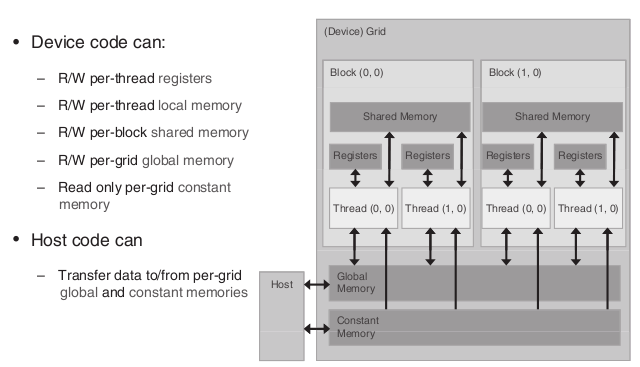
\includegraphics{MT.png}
\caption{This figure is from the website \href{http://www.elsevierdirect.com/v2/companion.jsp?ISBN=9780123814722}{http://www.elsevierdirect.com/v2/companion.jsp?ISBN=9780123814722}, originally found in the book \href{http://www.elsevierdirect.com/morgan\_kaufmann/kirk/}{Programming Massively Parallel Processors: A Hands-on Approach}.}\end{figure}

There are in total 4 types of memory designed for GPU cards with CUDA architecture. Global memory, located in the gird, has large storage capacity but limited speed, and can be read and write from all the blocks within CUDA system. Shared memory, located in each block, has small storage capacity (16KB per block) but fast accessing speed, can be read and write by all the threads within the located block. Constant memory, also located in the grid, has very small storage capacity (64KB per GPU) but very fast accessing speed, and can read (can't write) from any threads. There is also local memory located in each thread.


\begin{threeparttable}
\capstart\caption{CUDA Memory Types}

\begin{tabulary}{\linewidth}{|L|L|L|L|L|L|}
\hline
\textbf{
Memory
} & \textbf{
Scope of Access
} & \textbf{
Lifetime
} & \textbf{
R/W ability
} & \textbf{
Speed
} & \textbf{
Declaration
}\\\hline

Register
 & 
Thread
 & 
Kernel
 & 
R/W
 & 
Fast
 & 
Automatic Variables
\\\hline

Local
 & 
Thread
 & 
Kernel
 & 
R/W
 & 
Fast
 & 
Automatic Arrays
\\\hline

Shared
 & 
Block
 & 
Kernel
 & 
R/W
 & 
Fast
 & 
\_\_shared\_\_
\\\hline

Global
 & 
Grid
 & 
Host
 & 
R/W
 & 
Slow
 & 
\_\_device\_\_
\\\hline

Constant
 & 
Grid
 & 
Host
 & 
Read only
 & 
Fast
 & 
\_\_constant\_\_
\\\hline
\end{tabulary}

\end{threeparttable}



\bigskip\hrule{}\bigskip



\section{Shared Memory Version}
\label{CUDA2D/CUDA2D:tesla-c2075}\label{CUDA2D/CUDA2D:shared-memory-version}
Matrix Multiplication with Shared Memory source file:
\code{MM-GPU-SM.cu}

Why we need a shared memory version? We already seen hundreds of times speed improvement.

Well, to answer that question, we need to first look at the relationship between global memory and our program. That is, in order to finish the matrix multiplication, how many times each element in matrix is accessed in the global memory?

First, we have in total \emph{Width x Width} many of threads and each thread computes one element of the output matrix. Then, let's take a closer look at each thread. For example, thread with the threadIdx of (x,y) will computes the element in the x column and y row of the output matrix. In order to do this, thread (x,y) have to access elements in row x of matrix M and elements in column y of matrix N. How about thread (x,y+1)? This time kernel will have to access row x in matrix M again and a different column y+1 in matrix N. What about thread (x,y+2) or (x+1,y)? It is not hard for you to find out that we accessed each row in matrix M the \emph{Width} times and each column in matrix N the \emph{Width} times as well. If we can reduce the access time to once for every row in matrix M and once for every column in matrix N, we can not only save bandwidth, but also increase performance significantly.

Notice that although we say we want the kernel to access each row in matrix M and each column in matrix N once from global memory, we are not saying that the kernel access data once throughout the program. As we can see from previous sections, global memory has large capacity but low access speed. What we want is to transfer data from global memory to another type of memory which has fast access speed.

\begin{notice}{note}{Note:}
The kernel still need to access every row and every column \emph{Width} times in that memory location. However, as we are accessing them in a faster memory location, the time takes for those data to load will be significantly reduced. So technically we did not reduce the number of times each row or column was accessed, we simply made the speed of accessing them faster.
\end{notice}

Upon this point, it may occur to you that shared memory is the ideal candidate for such task for it can access data faster than global memory. However, shared memory also has the drawback of small storage capacity. In the case of matrix multiplication, we can't just store the whole matrix into the shared memory. Remember that shared memory only has 48kB storage space per block, which is not large enough for some gigantic matrices. We solve this problem by managing shared memory in a dynamically way.

In the previous example, we assigned \emph{Width x Width} many of threads for the computation where each thread will read one row of input matrix M and one column of input matrix N and computes the corresponding element in output matrix P. Although we use multiple blocks in a grid and multiple threads in a block, we don't see how threads are cooperating in the previous example. If we are allowed to assign infinite number of threads in one block, we can use just one block for the previous example. In this example, however, we will instruct all threads within one block to cooperate.
\begin{figure}[htbp]
\centering
\capstart

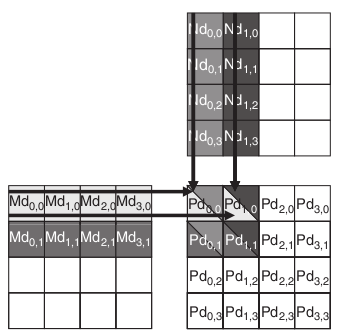
\includegraphics{MMSM1.png}
\caption{This figure is from the website \href{http://www.elsevierdirect.com/v2/companion.jsp?ISBN=9780123814722}{http://www.elsevierdirect.com/v2/companion.jsp?ISBN=9780123814722}, originally found in the book \href{http://www.elsevierdirect.com/morgan\_kaufmann/kirk/}{Programming Massively Parallel Processors: A Hands-on Approach}.}\end{figure}

In order to make the problem easier, we use two 4x4 matrices for illustration. We set the size of block as 2x2, which in total has 4 threads. Therefore, the output matrix will have 4 blocks. As shown in the \textbf{graph} above, each element of the output matrix is marked by Pd(x,y) where x is the column number and y is the row number. Lets take a look at the block which has element Pd(0,0),Pd(1,0),Pd(0,1) and Pd(1,1).

As you can see from graph, to compute four elements in this block, we need not only to access the corresponding block in input matrix M and input matrix N, but also the block to right of the corresponding block in matrix M and the block below the corresponding block in matrix N. That is in total 4 blocks of data need to be loaded. What if the maximum capacity of shared memory per block can only hold 2 blocks of data?

The solution is simple. All threads within a block can first collaborate together to load some portion of data from global memory. This can be easily done by every thread in the block load one element from both input matrices into shared memory. In our example, thread(0,0) loads Md(0,0) and Nd(0,0); thread(1,0) loads Md(1,0) and Nd(1,0); thread(0,1) loads Md(0,1) and Nd(0,1); finally threads(1,1) loads Md(1,1) and Nd(1,1).Then we use these data to do some computations in each thread even though this is enough to give the final results. We can always let each threads to remember the running sum. After the computation, We can delete the data in shared memory because we do not need them any more. Actually, you don't even need to \emph{delete} them, you can just load new data into it and old data will be erased automatically.

Then we can load more data from global memory to shared memory. This time, however, we cannot have each thread in the block load corresponding elements in input matrices. In our example, thread(0,0) loads Md(2,0) and Nd(0,2); thread(1,0) loads Md(3,0) and Nd(1,2); thread(0,1) loads Md(2,1) and Nd(0,3); finally threads(1,1) loads Md(3,1) and Nd(1,3). We can use this data for further computations. By the time we finished loading all the data to the shared memory from global memory, all the threads would have final results in the running sums. This way, we can use shared memory to increase the speed but not suffer from the limited storage capacity.
\begin{figure}[htbp]
\centering
\capstart

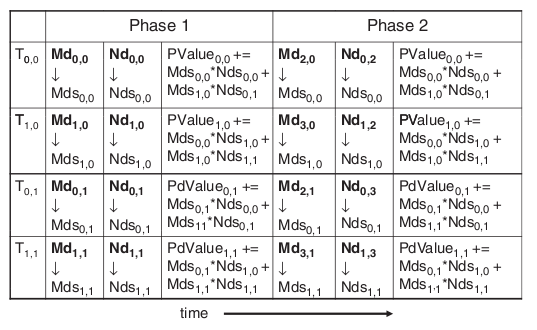
\includegraphics{MMSM2.png}
\caption{This figure is from the website \href{http://www.elsevierdirect.com/v2/companion.jsp?ISBN=9780123814722}{http://www.elsevierdirect.com/v2/companion.jsp?ISBN=9780123814722}, originally found in the book \href{http://www.elsevierdirect.com/morgan\_kaufmann/kirk/}{Programming Massively Parallel Processors: A Hands-on Approach}.}\end{figure}

We call each data loading and computing process a phase. Therefore, in the previous example, we went through 2 phases before we have our final results. It is not hard to find out that by using shared memory, we can reduce the number if times of accessing global memory from \emph{Width} times for every column or row to \emph{Width/blockDim} times.
1756.50
Back to our problem, we are dealing with input matrices with the size of \emph{1024 x 1024} and we are using blocks with the size of \emph{32 x 32}. We can potentially reduce the global memory accessing time to 1/32 of the original.


\subsection{The Device Code}
\label{CUDA2D/CUDA2D:id2}
\begin{Verbatim}[commandchars=\\\{\}]
\PYG{n}{\PYGZus{}\PYGZus{}global\PYGZus{}\PYGZus{}} \PYG{k+kt}{void} \PYG{n+nf}{MatrixMulKernel}\PYG{p}{(}\PYG{k+kt}{float}\PYG{o}{*} \PYG{n}{Md}\PYG{p}{,} \PYG{k+kt}{float}\PYG{o}{*} \PYG{n}{Nd}\PYG{p}{,} \PYG{k+kt}{float}\PYG{o}{*} \PYG{n}{Pd}\PYG{p}{,} \PYG{k+kt}{int} \PYG{n}{Width}\PYG{p}{)}
\PYG{p}{\PYGZob{}}
  \PYG{c+c1}{// declare cache in the shared memory}
  \PYG{n}{\PYGZus{}\PYGZus{}shared\PYGZus{}\PYGZus{}} \PYG{k+kt}{float} \PYG{n}{Mds}\PYG{p}{[}\PYG{n}{blockD}\PYG{p}{]}\PYG{p}{[}\PYG{n}{blockD}\PYG{p}{]}\PYG{p}{;}
  \PYG{n}{\PYGZus{}\PYGZus{}shared\PYGZus{}\PYGZus{}} \PYG{k+kt}{float} \PYG{n}{Nds}\PYG{p}{[}\PYG{n}{blockD}\PYG{p}{]}\PYG{p}{[}\PYG{n}{blockD}\PYG{p}{]}\PYG{p}{;}
 
  \PYG{c+c1}{// keep track of column index of the Pd element using thread index}
  \PYG{k+kt}{int} \PYG{n}{x} \PYG{o}{=} \PYG{n}{threadIdx}\PYG{p}{.}\PYG{n}{x} \PYG{o}{+} \PYG{n}{blockIdx}\PYG{p}{.}\PYG{n}{x} \PYG{o}{*} \PYG{n}{blockDim}\PYG{p}{.}\PYG{n}{x}\PYG{p}{;} \PYG{c+c1}{// x is column}
  \PYG{c+c1}{// keep track of row index of the Pd element using thread index}
  \PYG{k+kt}{int} \PYG{n}{y} \PYG{o}{=} \PYG{n}{threadIdx}\PYG{p}{.}\PYG{n}{y} \PYG{o}{+} \PYG{n}{blockIdx}\PYG{p}{.}\PYG{n}{y} \PYG{o}{*} \PYG{n}{blockDim}\PYG{p}{.}\PYG{n}{y}\PYG{p}{;} \PYG{c+c1}{// y is row}

  \PYG{k+kt}{float} \PYG{n}{Pvalue} \PYG{o}{=} \PYG{l+m+mi}{0}\PYG{p}{;}
  \PYG{c+c1}{// Loop over the Md and Nd block dimension required to compute the Pd element}
  \PYG{k}{for} \PYG{p}{(}\PYG{k+kt}{int} \PYG{n}{m} \PYG{o}{=} \PYG{l+m+mi}{0}\PYG{p}{;} \PYG{n}{m} \PYG{o}{\PYGZlt{}} \PYG{n}{Width}\PYG{o}{/}\PYG{n}{blockD}\PYG{p}{;} \PYG{n}{m}\PYG{o}{+}\PYG{o}{+}\PYG{p}{)}\PYG{p}{\PYGZob{}}
	
    \PYG{c+c1}{// collaboratively loading of Md and Nd blocks into shared memory	 }
    \PYG{n}{Mds}\PYG{p}{[}\PYG{n}{threadIdx}\PYG{p}{.}\PYG{n}{y}\PYG{p}{]}\PYG{p}{[}\PYG{n}{threadIdx}\PYG{p}{.}\PYG{n}{x}\PYG{p}{]} \PYG{o}{=} \PYG{n}{Md}\PYG{p}{[}\PYG{n}{y} \PYG{o}{*} \PYG{n}{Width} \PYG{o}{+} \PYG{p}{(}\PYG{n}{m} \PYG{o}{*} \PYG{n}{blockD} \PYG{o}{+} \PYG{n}{threadIdx}\PYG{p}{.}\PYG{n}{x}\PYG{p}{)}\PYG{p}{]}\PYG{p}{;}
    \PYG{n}{Nds}\PYG{p}{[}\PYG{n}{threadIdx}\PYG{p}{.}\PYG{n}{y}\PYG{p}{]}\PYG{p}{[}\PYG{n}{threadIdx}\PYG{p}{.}\PYG{n}{x}\PYG{p}{]} \PYG{o}{=} \PYG{n}{Md}\PYG{p}{[}\PYG{p}{(}\PYG{n}{m} \PYG{o}{*} \PYG{n}{blockD} \PYG{o}{+} \PYG{n}{threadIdx}\PYG{p}{.}\PYG{n}{y}\PYG{p}{)} \PYG{o}{*} \PYG{n}{Width} \PYG{o}{+} \PYG{n}{x}\PYG{p}{]}\PYG{p}{;}
    \PYG{n}{\PYGZus{}\PYGZus{}syncthreads}\PYG{p}{(}\PYG{p}{)}\PYG{p}{;}
    
    \PYG{c+c1}{// keep track of the running sum    }
    \PYG{k}{for} \PYG{p}{(}\PYG{k+kt}{int} \PYG{n}{k} \PYG{o}{=} \PYG{l+m+mi}{0}\PYG{p}{;} \PYG{n}{k} \PYG{o}{\PYGZlt{}} \PYG{n}{blockD}\PYG{p}{;} \PYG{n}{k}\PYG{o}{+}\PYG{o}{+}\PYG{p}{)}
      \PYG{n}{Pvalue} \PYG{o}{+}\PYG{o}{=} \PYG{n}{Mds}\PYG{p}{[}\PYG{n}{threadIdx}\PYG{p}{.}\PYG{n}{y}\PYG{p}{]}\PYG{p}{[}\PYG{n}{k}\PYG{p}{]} \PYG{o}{*} \PYG{n}{Nds}\PYG{p}{[}\PYG{n}{k}\PYG{p}{]}\PYG{p}{[}\PYG{n}{threadIdx}\PYG{p}{.}\PYG{n}{x}\PYG{p}{]}\PYG{p}{;}
    \PYG{n}{\PYGZus{}\PYGZus{}syncthreads}\PYG{p}{(}\PYG{p}{)}\PYG{p}{;}
  \PYG{p}{\PYGZcb{}}
  
  \PYG{c+c1}{// write back to the global memory}
  \PYG{n}{Pd}\PYG{p}{[}\PYG{n}{y} \PYG{o}{*} \PYG{n}{Width} \PYG{o}{+} \PYG{n}{x}\PYG{p}{]} \PYG{o}{=} \PYG{n}{Pvalue}\PYG{p}{;}
\PYG{p}{\PYGZcb{}}
\end{Verbatim}

With all the explanations before, you should understand this device code easily.

If you are careful enough, you may see that I used a variable called \textbf{blockD}. This variable was defined at the very beginning of the source code.

\begin{Verbatim}[commandchars=\\\{\}]
\PYG{c+cp}{\PYGZsh{}}\PYG{c+cp}{define blockD 32}
\end{Verbatim}

There are two thing you need to pay attention when defining this variable. First is that you should not assign this variable with a number that is too big. This variable is used to define the dimension of each block. The reason we are using block is to reduce the size of data transfer between global memory and shared memory every time. If you assign too big a number to it, you are risking running out of share memory.

Another thing is that some of you might wonder why we are using \emph{blockD} to represent block dimension instead of using blockDim. Well, blockDim is a built-in function used by CUDA C, you can define blockDim as a constant in here, but the built-in function will fail if you call it since you define a function equals a constant. The point I am trying to make here is that be very careful when you are choosing your variable names. CUDA C, different from standard C, has more built-in functions and you might bump into one or two while you are naming variables.


\subsection{About blockDim and matrix dimension}
\label{CUDA2D/CUDA2D:about-blockdim-and-matrix-dimension}
Another thing needs mentioning is that while choosing the value of \emph{blockD}, it is crucial for you to reference the matrix dimension before you decide which number to assign to \emph{blockD}. Different from the global memory version and CPU version, shared memory version requires threads within a block to work collaboratively to load part of the data to shared memory each time. This means matrix's dimension should be multiples of \emph{blockD} so that threads in a block can load same amount of data each time.

Further, recall that in the device code, we have expression like

\begin{Verbatim}[commandchars=\\\{\}]
  \PYG{k}{for} \PYG{p}{(}\PYG{k+kt}{int} \PYG{n}{m} \PYG{o}{=} \PYG{l+m+mi}{0}\PYG{p}{;} \PYG{n}{m} \PYG{o}{\PYGZlt{}} \PYG{n}{Width}\PYG{o}{/}\PYG{n}{blockD}\PYG{p}{;} \PYG{n}{m}\PYG{o}{+}\PYG{o}{+}\PYG{p}{)}\PYG{p}{\PYGZob{}}
\end{Verbatim}

where we have \emph{Width} divided by \emph{blockD}. If you pick \emph{Width} that is not dividable by \emph{blockD}, program will return weird thing because it expects a integer coming out of this line of code, instead of some floats.

As this program is using 1024 as \emph{Width}, we picked 32 as the \emph{blockD} value. If you use 1000 instead if 1024 for \emph{Width} and print out the result, you will see weird results. However, if you happen to have matrices with dimension of 1000, you should use 25 instead of 32 as the \emph{blockD} value.


\subsection{The Host Code}
\label{CUDA2D/CUDA2D:id3}
\begin{Verbatim}[commandchars=\\\{\}]
\PYG{n}{main}\PYG{p}{(}\PYG{k+kt}{void}\PYG{p}{)}\PYG{p}{\PYGZob{}}

    \PYG{k+kt}{void} \PYG{n}{MatrixMultiplication}\PYG{p}{(}\PYG{k+kt}{float} \PYG{o}{*}\PYG{p}{,} \PYG{k+kt}{float} \PYG{o}{*}\PYG{p}{,} \PYG{k+kt}{float} \PYG{o}{*}\PYG{p}{,} \PYG{k+kt}{int}\PYG{p}{)}\PYG{p}{;}

    \PYG{k}{const} \PYG{k+kt}{int} \PYG{n}{Width} \PYG{o}{=} \PYG{l+m+mi}{1024}\PYG{p}{;}

    \PYG{k+kt}{int} \PYG{n}{size} \PYG{o}{=} \PYG{n}{Width} \PYG{o}{*} \PYG{n}{Width} \PYG{o}{*} \PYG{k}{sizeof}\PYG{p}{(}\PYG{k+kt}{float}\PYG{p}{)}\PYG{p}{;}
    \PYG{k+kt}{float} \PYG{o}{*}\PYG{n}{M}\PYG{p}{,} \PYG{o}{*}\PYG{n}{N}\PYG{p}{,} \PYG{o}{*}\PYG{n}{P}\PYG{p}{;}   
    
    \PYG{c+c1}{// allocate memory on the CPU}
    \PYG{n}{M} \PYG{o}{=} \PYG{p}{(}\PYG{k+kt}{float}\PYG{o}{*}\PYG{p}{)}\PYG{n}{malloc}\PYG{p}{(}\PYG{n}{size}\PYG{p}{)}\PYG{p}{;}
    \PYG{n}{N} \PYG{o}{=} \PYG{p}{(}\PYG{k+kt}{float}\PYG{o}{*}\PYG{p}{)}\PYG{n}{malloc}\PYG{p}{(}\PYG{n}{size}\PYG{p}{)}\PYG{p}{;}
    \PYG{n}{P} \PYG{o}{=} \PYG{p}{(}\PYG{k+kt}{float}\PYG{o}{*}\PYG{p}{)}\PYG{n}{malloc}\PYG{p}{(}\PYG{n}{size}\PYG{p}{)}\PYG{p}{;}

    \PYG{c+c1}{// initialize the matrices}
    \PYG{k}{for} \PYG{p}{(}\PYG{k+kt}{int} \PYG{n}{y}\PYG{o}{=}\PYG{l+m+mi}{0}\PYG{p}{;} \PYG{n}{y}\PYG{o}{\PYGZlt{}}\PYG{n}{Width}\PYG{p}{;} \PYG{n}{y}\PYG{o}{+}\PYG{o}{+}\PYG{p}{)} \PYG{p}{\PYGZob{}}
	    \PYG{k}{for} \PYG{p}{(}\PYG{k+kt}{int} \PYG{n}{x}\PYG{o}{=}\PYG{l+m+mi}{0}\PYG{p}{;} \PYG{n}{x}\PYG{o}{\PYGZlt{}}\PYG{n}{Width}\PYG{p}{;} \PYG{n}{x}\PYG{o}{+}\PYG{o}{+}\PYG{p}{)}\PYG{p}{\PYGZob{}}
	   		\PYG{n}{M}\PYG{p}{[}\PYG{n}{y}\PYG{o}{*}\PYG{n}{Width} \PYG{o}{+} \PYG{n}{x}\PYG{p}{]} \PYG{o}{=} \PYG{n}{x} \PYG{o}{+} \PYG{n}{y}\PYG{o}{*}\PYG{n}{Width}\PYG{p}{;}
       		\PYG{n}{N}\PYG{p}{[}\PYG{n}{y}\PYG{o}{*}\PYG{n}{Width} \PYG{o}{+} \PYG{n}{x}\PYG{p}{]} \PYG{o}{=} \PYG{n}{x} \PYG{o}{+} \PYG{n}{y}\PYG{o}{*}\PYG{n}{Width}\PYG{p}{;} 
	   \PYG{p}{\PYGZcb{}}
    \PYG{p}{\PYGZcb{}}

    \PYG{n}{MatrixMultiplication}\PYG{p}{(}\PYG{n}{M}\PYG{p}{,} \PYG{n}{N}\PYG{p}{,} \PYG{n}{P}\PYG{p}{,} \PYG{n}{Width}\PYG{p}{)}\PYG{p}{;}

    \PYG{c+c1}{// free the memory allocated on the CPU}
    \PYG{n}{free}\PYG{p}{(} \PYG{n}{M} \PYG{p}{)}\PYG{p}{;}
    \PYG{n}{free}\PYG{p}{(} \PYG{n}{N} \PYG{p}{)}\PYG{p}{;}
    \PYG{n}{free}\PYG{p}{(} \PYG{n}{P} \PYG{p}{)}\PYG{p}{;}

    \PYG{k}{return} \PYG{l+m+mi}{0}\PYG{p}{;}
\PYG{p}{\PYGZcb{}}
\PYG{n}{\PYGZus{}\PYGZus{}global\PYGZus{}\PYGZus{}} \PYG{k+kt}{void} \PYG{n}{MatrixMulKernel}\PYG{p}{(}\PYG{k+kt}{float}\PYG{o}{*} \PYG{n}{Md}\PYG{p}{,} \PYG{k+kt}{float}\PYG{o}{*} \PYG{n}{Nd}\PYG{p}{,} \PYG{k+kt}{float}\PYG{o}{*} \PYG{n}{Pd}\PYG{p}{,} \PYG{k+kt}{int} \PYG{n}{Width}\PYG{p}{)}
\PYG{p}{\PYGZob{}}
  \PYG{c+c1}{// declare cache in the shared memory}
  \PYG{n}{\PYGZus{}\PYGZus{}shared\PYGZus{}\PYGZus{}} \PYG{k+kt}{float} \PYG{n}{Mds}\PYG{p}{[}\PYG{n}{blockD}\PYG{p}{]}\PYG{p}{[}\PYG{n}{blockD}\PYG{p}{]}\PYG{p}{;}
  \PYG{n}{\PYGZus{}\PYGZus{}shared\PYGZus{}\PYGZus{}} \PYG{k+kt}{float} \PYG{n}{Nds}\PYG{p}{[}\PYG{n}{blockD}\PYG{p}{]}\PYG{p}{[}\PYG{n}{blockD}\PYG{p}{]}\PYG{p}{;}
 
  \PYG{c+c1}{// keep track of column index of the Pd element using thread index}
  \PYG{k+kt}{int} \PYG{n}{x} \PYG{o}{=} \PYG{n}{threadIdx}\PYG{p}{.}\PYG{n}{x} \PYG{o}{+} \PYG{n}{blockIdx}\PYG{p}{.}\PYG{n}{x} \PYG{o}{*} \PYG{n}{blockDim}\PYG{p}{.}\PYG{n}{x}\PYG{p}{;} \PYG{c+c1}{// x is column}
  \PYG{c+c1}{// keep track of row index of the Pd element using thread index}
  \PYG{k+kt}{int} \PYG{n}{y} \PYG{o}{=} \PYG{n}{threadIdx}\PYG{p}{.}\PYG{n}{y} \PYG{o}{+} \PYG{n}{blockIdx}\PYG{p}{.}\PYG{n}{y} \PYG{o}{*} \PYG{n}{blockDim}\PYG{p}{.}\PYG{n}{y}\PYG{p}{;} \PYG{c+c1}{// y is row}

  \PYG{k+kt}{float} \PYG{n}{Pvalue} \PYG{o}{=} \PYG{l+m+mi}{0}\PYG{p}{;}
  \PYG{c+c1}{// Loop over the Md and Nd block dimension required to compute the Pd element}
  \PYG{k}{for} \PYG{p}{(}\PYG{k+kt}{int} \PYG{n}{m} \PYG{o}{=} \PYG{l+m+mi}{0}\PYG{p}{;} \PYG{n}{m} \PYG{o}{\PYGZlt{}} \PYG{n}{Width}\PYG{o}{/}\PYG{n}{blockD}\PYG{p}{;} \PYG{n}{m}\PYG{o}{+}\PYG{o}{+}\PYG{p}{)}\PYG{p}{\PYGZob{}}
	
    \PYG{c+c1}{// collaboratively loading of Md and Nd blocks into shared memory	 }
    \PYG{n}{Mds}\PYG{p}{[}\PYG{n}{threadIdx}\PYG{p}{.}\PYG{n}{y}\PYG{p}{]}\PYG{p}{[}\PYG{n}{threadIdx}\PYG{p}{.}\PYG{n}{x}\PYG{p}{]} \PYG{o}{=} \PYG{n}{Md}\PYG{p}{[}\PYG{n}{y} \PYG{o}{*} \PYG{n}{Width} \PYG{o}{+} \PYG{p}{(}\PYG{n}{m} \PYG{o}{*} \PYG{n}{blockD} \PYG{o}{+} \PYG{n}{threadIdx}\PYG{p}{.}\PYG{n}{x}\PYG{p}{)}\PYG{p}{]}\PYG{p}{;}
    \PYG{n}{Nds}\PYG{p}{[}\PYG{n}{threadIdx}\PYG{p}{.}\PYG{n}{y}\PYG{p}{]}\PYG{p}{[}\PYG{n}{threadIdx}\PYG{p}{.}\PYG{n}{x}\PYG{p}{]} \PYG{o}{=} \PYG{n}{Md}\PYG{p}{[}\PYG{p}{(}\PYG{n}{m} \PYG{o}{*} \PYG{n}{blockD} \PYG{o}{+} \PYG{n}{threadIdx}\PYG{p}{.}\PYG{n}{y}\PYG{p}{)} \PYG{o}{*} \PYG{n}{Width} \PYG{o}{+} \PYG{n}{x}\PYG{p}{]}\PYG{p}{;}
    \PYG{n}{\PYGZus{}\PYGZus{}syncthreads}\PYG{p}{(}\PYG{p}{)}\PYG{p}{;}
    
    \PYG{c+c1}{// keep track of the running sum    }
    \PYG{k}{for} \PYG{p}{(}\PYG{k+kt}{int} \PYG{n}{k} \PYG{o}{=} \PYG{l+m+mi}{0}\PYG{p}{;} \PYG{n}{k} \PYG{o}{\PYGZlt{}} \PYG{n}{blockD}\PYG{p}{;} \PYG{n}{k}\PYG{o}{+}\PYG{o}{+}\PYG{p}{)}
      \PYG{n}{Pvalue} \PYG{o}{+}\PYG{o}{=} \PYG{n}{Mds}\PYG{p}{[}\PYG{n}{threadIdx}\PYG{p}{.}\PYG{n}{y}\PYG{p}{]}\PYG{p}{[}\PYG{n}{k}\PYG{p}{]} \PYG{o}{*} \PYG{n}{Nds}\PYG{p}{[}\PYG{n}{k}\PYG{p}{]}\PYG{p}{[}\PYG{n}{threadIdx}\PYG{p}{.}\PYG{n}{x}\PYG{p}{]}\PYG{p}{;}
    \PYG{n}{\PYGZus{}\PYGZus{}syncthreads}\PYG{p}{(}\PYG{p}{)}\PYG{p}{;}
  \PYG{p}{\PYGZcb{}}
  
  \PYG{c+c1}{// write back to the global memory}
  \PYG{n}{Pd}\PYG{p}{[}\PYG{n}{y} \PYG{o}{*} \PYG{n}{Width} \PYG{o}{+} \PYG{n}{x}\PYG{p}{]} \PYG{o}{=} \PYG{n}{Pvalue}\PYG{p}{;}
\PYG{p}{\PYGZcb{}}

\PYG{k+kt}{void} \PYG{n}{MatrixMultiplication}\PYG{p}{(}\PYG{k+kt}{float} \PYG{o}{*}\PYG{n}{M}\PYG{p}{,} \PYG{k+kt}{float} \PYG{o}{*}\PYG{n}{N}\PYG{p}{,} \PYG{k+kt}{float} \PYG{o}{*}\PYG{n}{P}\PYG{p}{,} \PYG{k+kt}{int} \PYG{n}{Width}\PYG{p}{)} \PYG{p}{\PYGZob{}}

    \PYG{k+kt}{int} \PYG{n}{size} \PYG{o}{=} \PYG{n}{Width} \PYG{o}{*} \PYG{n}{Width} \PYG{o}{*} \PYG{k}{sizeof}\PYG{p}{(}\PYG{k+kt}{float}\PYG{p}{)}\PYG{p}{;}
    \PYG{k+kt}{float} \PYG{o}{*}\PYG{n}{Md}\PYG{p}{,} \PYG{o}{*}\PYG{n}{Nd}\PYG{p}{,} \PYG{o}{*}\PYG{n}{Pd}\PYG{p}{;} 

    \PYG{c+c1}{// capture start time}
    \PYG{n}{cudaEvent\PYGZus{}t}     \PYG{n}{start}\PYG{p}{,} \PYG{n}{stop}\PYG{p}{;}
    \PYG{n}{HANDLE\PYGZus{}ERROR}\PYG{p}{(} \PYG{n}{cudaEventCreate}\PYG{p}{(} \PYG{o}{\PYGZam{}}\PYG{n}{start} \PYG{p}{)} \PYG{p}{)}\PYG{p}{;}
    \PYG{n}{HANDLE\PYGZus{}ERROR}\PYG{p}{(} \PYG{n}{cudaEventCreate}\PYG{p}{(} \PYG{o}{\PYGZam{}}\PYG{n}{stop} \PYG{p}{)} \PYG{p}{)}\PYG{p}{;}
    \PYG{n}{HANDLE\PYGZus{}ERROR}\PYG{p}{(} \PYG{n}{cudaEventRecord}\PYG{p}{(} \PYG{n}{start}\PYG{p}{,} \PYG{l+m+mi}{0} \PYG{p}{)} \PYG{p}{)}\PYG{p}{;}

    \PYG{c+c1}{// allocate memory on the GPU}
    \PYG{n}{HANDLE\PYGZus{}ERROR}\PYG{p}{(} \PYG{n}{cudaMalloc}\PYG{p}{(}\PYG{p}{(}\PYG{k+kt}{void}\PYG{o}{*}\PYG{o}{*}\PYG{p}{)}\PYG{o}{\PYGZam{}}\PYG{n}{Md}\PYG{p}{,} \PYG{n}{size}\PYG{p}{)} \PYG{p}{)}\PYG{p}{;}
    \PYG{n}{HANDLE\PYGZus{}ERROR}\PYG{p}{(} \PYG{n}{cudaMalloc}\PYG{p}{(}\PYG{p}{(}\PYG{k+kt}{void}\PYG{o}{*}\PYG{o}{*}\PYG{p}{)}\PYG{o}{\PYGZam{}}\PYG{n}{Nd}\PYG{p}{,} \PYG{n}{size}\PYG{p}{)} \PYG{p}{)}\PYG{p}{;}
    \PYG{n}{HANDLE\PYGZus{}ERROR}\PYG{p}{(} \PYG{n}{cudaMalloc}\PYG{p}{(}\PYG{p}{(}\PYG{k+kt}{void}\PYG{o}{*}\PYG{o}{*}\PYG{p}{)}\PYG{o}{\PYGZam{}}\PYG{n}{Pd}\PYG{p}{,} \PYG{n}{size}\PYG{p}{)} \PYG{p}{)}\PYG{p}{;}

    \PYG{c+c1}{// transfer M and N to device memory}
    \PYG{n}{HANDLE\PYGZus{}ERROR}\PYG{p}{(} \PYG{n}{cudaMemcpy}\PYG{p}{(}\PYG{n}{Md}\PYG{p}{,} \PYG{n}{M}\PYG{p}{,} \PYG{n}{size}\PYG{p}{,} \PYG{n}{cudaMemcpyHostToDevice}\PYG{p}{)} \PYG{p}{)}\PYG{p}{;}
    \PYG{n}{HANDLE\PYGZus{}ERROR}\PYG{p}{(} \PYG{n}{cudaMemcpy}\PYG{p}{(}\PYG{n}{Nd}\PYG{p}{,} \PYG{n}{N}\PYG{p}{,} \PYG{n}{size}\PYG{p}{,} \PYG{n}{cudaMemcpyHostToDevice}\PYG{p}{)} \PYG{p}{)}\PYG{p}{;}

    \PYG{c+c1}{// kernel invocation code}
    \PYG{n}{dim3} \PYG{n}{dimBlock}\PYG{p}{(}\PYG{n}{blockD}\PYG{p}{,} \PYG{n}{blockD}\PYG{p}{)}\PYG{p}{;}
    \PYG{n}{dim3} \PYG{n}{dimGrid}\PYG{p}{(}\PYG{n}{Width}\PYG{o}{/}\PYG{n}{blockD}\PYG{p}{,} \PYG{n}{Width}\PYG{o}{/}\PYG{n}{blockD}\PYG{p}{)}\PYG{p}{;}
    \PYG{n}{MatrixMulKernel}\PYG{o}{\PYGZlt{}}\PYG{o}{\PYGZlt{}}\PYG{o}{\PYGZlt{}}\PYG{n}{dimGrid}\PYG{p}{,} \PYG{n}{dimBlock}\PYG{o}{\PYGZgt{}}\PYG{o}{\PYGZgt{}}\PYG{o}{\PYGZgt{}}\PYG{p}{(} \PYG{n}{Md}\PYG{p}{,} \PYG{n}{Nd}\PYG{p}{,} \PYG{n}{Pd}\PYG{p}{,} \PYG{n}{Width}\PYG{p}{)}\PYG{p}{;}

    \PYG{c+c1}{// transfer P from device    }
    \PYG{n}{HANDLE\PYGZus{}ERROR}\PYG{p}{(} \PYG{n}{cudaMemcpy}\PYG{p}{(}\PYG{n}{P}\PYG{p}{,} \PYG{n}{Pd}\PYG{p}{,} \PYG{n}{size}\PYG{p}{,} \PYG{n}{cudaMemcpyDeviceToHost}\PYG{p}{)} \PYG{p}{)}\PYG{p}{;}

    \PYG{c+c1}{// get stop time, and display the timing results}
    \PYG{n}{HANDLE\PYGZus{}ERROR}\PYG{p}{(} \PYG{n}{cudaEventRecord}\PYG{p}{(} \PYG{n}{stop}\PYG{p}{,} \PYG{l+m+mi}{0} \PYG{p}{)} \PYG{p}{)}\PYG{p}{;}
    \PYG{n}{HANDLE\PYGZus{}ERROR}\PYG{p}{(} \PYG{n}{cudaEventSynchronize}\PYG{p}{(} \PYG{n}{stop} \PYG{p}{)} \PYG{p}{)}\PYG{p}{;}
    \PYG{k+kt}{float}   \PYG{n}{elapsedTime}\PYG{p}{;}
    \PYG{n}{HANDLE\PYGZus{}ERROR}\PYG{p}{(} \PYG{n}{cudaEventElapsedTime}\PYG{p}{(} \PYG{o}{\PYGZam{}}\PYG{n}{elapsedTime}\PYG{p}{,}
                                        \PYG{n}{start}\PYG{p}{,} \PYG{n}{stop} \PYG{p}{)} \PYG{p}{)}\PYG{p}{;}
    \PYG{n}{printf}\PYG{p}{(} \PYG{l+s}{"}\PYG{l+s}{Time to generate:  \PYGZpc{}3.1f ms}\PYG{l+s+se}{\PYGZbs{}n}\PYG{l+s}{"}\PYG{p}{,} \PYG{n}{elapsedTime} \PYG{p}{)}\PYG{p}{;}

    \PYG{c+c1}{// free the memory allocated on the GPU}
    \PYG{n}{HANDLE\PYGZus{}ERROR}\PYG{p}{(} \PYG{n}{cudaFree}\PYG{p}{(}\PYG{n}{Md}\PYG{p}{)} \PYG{p}{)}\PYG{p}{;}
    \PYG{n}{HANDLE\PYGZus{}ERROR}\PYG{p}{(} \PYG{n}{cudaFree}\PYG{p}{(}\PYG{n}{Nd}\PYG{p}{)} \PYG{p}{)}\PYG{p}{;}
    \PYG{n}{HANDLE\PYGZus{}ERROR}\PYG{p}{(} \PYG{n}{cudaFree}\PYG{p}{(}\PYG{n}{Pd}\PYG{p}{)} \PYG{p}{)}\PYG{p}{;}

    \PYG{c+c1}{// destroy events to free memory}
    \PYG{n}{HANDLE\PYGZus{}ERROR}\PYG{p}{(} \PYG{n}{cudaEventDestroy}\PYG{p}{(} \PYG{n}{start} \PYG{p}{)} \PYG{p}{)}\PYG{p}{;}
    \PYG{n}{HANDLE\PYGZus{}ERROR}\PYG{p}{(} \PYG{n}{cudaEventDestroy}\PYG{p}{(} \PYG{n}{stop} \PYG{p}{)} \PYG{p}{)}\PYG{p}{;}
\PYG{p}{\PYGZcb{}}
\end{Verbatim}

There is nothing worth mentioning in the host code because it is almost identical to what we had in the previous example.


\subsection{Performance}
\label{CUDA2D/CUDA2D:id4}
While testing the performance, we used 1024 as Width same as the number used in the CPU baseline program. We conducted 5 tests and the results are below.
\begin{itemize}
\item {} \begin{enumerate}
\item {} 
24.4 ms

\end{enumerate}

\item {} \begin{enumerate}
\setcounter{enumi}{1}
\item {} 
24.2 ms

\end{enumerate}

\item {} \begin{enumerate}
\setcounter{enumi}{2}
\item {} 
24.3 ms

\end{enumerate}

\item {} \begin{enumerate}
\setcounter{enumi}{3}
\item {} 
24.4 ms

\end{enumerate}

\item {} \begin{enumerate}
\setcounter{enumi}{4}
\item {} 
24.4 ms

\end{enumerate}

\item {} 
Average: 24.34 ms

\end{itemize}

Compared the CPU program, our GPU program is \textbf{1664} times faster.


\chapter{Ray Tracing and Constant Memory}
\label{RTACM/RTACM::doc}\label{RTACM/RTACM:ray-tracing-and-constant-memory}

\section{Acknowledgement}
\label{RTACM/RTACM:acknowledgement}
The examples used in this chapter are based on examples in \href{http://developer.nvidia.com/content/cuda-example-introduction-general-purpose-gpu-programming-0}{CUDA BY EXAMPLE: An Introduction to General-Purpose GPU Programming}, written by Jason Sanders and Edward Kandrot, and published by Addison Wesley.

Copyright 1993-2010 NVIDIA Corporation.  All rights reserved.

This copy of code is a derivative based on the original code and designed for educational purposes only. It contains source code provided by \href{http://www.nvidia.com}{NVIDIA Corporation}.


\section{Basics of Ray Tracing}
\label{RTACM/RTACM:nvidia-corporation}\label{RTACM/RTACM:basics-of-ray-tracing}
First of all, what is ray tracing. Well, ray tracing is how you reflect a scene consisting three-dimensional objects on a two dimensional image. This is similar to the games you play on your computer, except your games might use a different method. However, the basic idea behind is the same.

How does ray tracing work? It is actually pretty simple. In the two-dimensional image, you place a imaginary camera in there. Just like most real cameras, this imaginary camera contains light sensor as well. To produce a image, all we have to do is determine what light would hit our camera. The camera, on the other hand, would automatically record the color and light intensity of the ray hit it and produce exact same color and light intensity on the corresponding pixel.

Furthermore, deciding which ray would hit the camera is painstaking. So our clever computer scientist came up with an idea. Rather than deciding which ray would hit our camera, we can imagine shooting out a ray from our camera into the scene consisting three-dimensional objects. In other words, our imaginary camera is acting as an eye and we are now trying to find out what the eye is looking at. To seen what the eye is seeing, all we need to do is trace the ray shot out from the camera until it hits an object in our three-dimensional scene. We then record the color of the object and assign the color to the pixel. As you can see, most of the work in ray tracing is just deciding how the rays shot out and the objects in the scene would interact.


\section{Notes for Compile}
\label{RTACM/RTACM:notes-for-compile}
Before this chapter, we use the following code to compile CUDA code.

\textbf{\textgreater{} nvcc -o example\_name example\_name.cu}

However, since we are using CUDA to produce images in this chapter, we need to use different code for compiling. Shown as follow

\textbf{\textgreater{} nvcc -lglut -o example\_name example\_name.c}


\section{Ray Tracing Without Constant Memory}
\label{RTACM/RTACM:ray-tracing-without-constant-memory}
In our example, we will create a scene with 20 random spheres. They are placed in a cube with dimension 1000 x 1000 x 1000. The center of the cube is at the origin. All the spheres are random in size, position as well as color. We then place the camera on a random place on z-axis and fix it facing origin. Later on, all we need to do is to fire a ray from each pixel and keep tracing it until it hits one of the objects. We also need to keep track of the depth of the ray. Since one ray can hit more than one objects, we only need to record the nearest object and its color.

Ray Tracing Without Constant Memory source file:
\code{ray\_noconst.cu}


\subsection{Structure Code}
\label{RTACM/RTACM:structure-code}
We first create a data structure Sphere. Just like standard C, you can also create data structures in CUDA C.

\begin{Verbatim}[commandchars=\\\{\}]
\PYG{k}{struct} \PYG{n}{Sphere} \PYG{p}{\PYGZob{}}

    \PYG{k+kt}{float}   \PYG{n}{r}\PYG{p}{,}\PYG{n}{b}\PYG{p}{,}\PYG{n}{g}\PYG{p}{;}\PYG{c+c1}{// color of the sphere}
    \PYG{k+kt}{float}   \PYG{n}{radius}\PYG{p}{;} 
    \PYG{k+kt}{float}   \PYG{n}{x}\PYG{p}{,}\PYG{n}{y}\PYG{p}{,}\PYG{n}{z}\PYG{p}{;}\PYG{c+c1}{// coordinate of the center}
    
    \PYG{c+c1}{// will return the distance between imaginary camera and hit}
    \PYG{n}{\PYGZus{}\PYGZus{}device\PYGZus{}\PYGZus{}} \PYG{k+kt}{float} \PYG{n+nf}{hit}\PYG{p}{(} \PYG{k+kt}{float} \PYG{n}{ox}\PYG{p}{,} \PYG{k+kt}{float} \PYG{n}{oy}\PYG{p}{,} \PYG{k+kt}{float} \PYG{o}{*}\PYG{n}{n} \PYG{p}{)} \PYG{p}{\PYGZob{}}
        \PYG{k+kt}{float} \PYG{n}{dx} \PYG{o}{=} \PYG{n}{ox} \PYG{o}{-} \PYG{n}{x}\PYG{p}{;} \PYG{c+c1}{// distance on x-axis}
        \PYG{k+kt}{float} \PYG{n}{dy} \PYG{o}{=} \PYG{n}{oy} \PYG{o}{-} \PYG{n}{y}\PYG{p}{;} \PYG{c+c1}{// distance on y-axis}
        \PYG{c+c1}{// if (dx*dx + dy*dy \PYGZgt{} radius*radius), ray will not hit sphere}
        \PYG{k}{if} \PYG{p}{(}\PYG{n}{dx}\PYG{o}{*}\PYG{n}{dx} \PYG{o}{+} \PYG{n}{dy}\PYG{o}{*}\PYG{n}{dy} \PYG{o}{\PYGZlt{}} \PYG{n}{radius}\PYG{o}{*}\PYG{n}{radius}\PYG{p}{)} \PYG{p}{\PYGZob{}}
            \PYG{k+kt}{float} \PYG{n}{dz} \PYG{o}{=} \PYG{n}{sqrtf}\PYG{p}{(} \PYG{n}{radius}\PYG{o}{*}\PYG{n}{radius} \PYG{o}{-} \PYG{n}{dx}\PYG{o}{*}\PYG{n}{dx} \PYG{o}{-} \PYG{n}{dy}\PYG{o}{*}\PYG{n}{dy} \PYG{p}{)}\PYG{p}{;}
            \PYG{c+c1}{// n is used in visual effect}
            \PYG{o}{*}\PYG{n}{n} \PYG{o}{=} \PYG{n}{dz} \PYG{o}{/} \PYG{n}{sqrtf}\PYG{p}{(} \PYG{n}{radius} \PYG{o}{*} \PYG{n}{radius} \PYG{p}{)}\PYG{p}{;}
            \PYG{k}{return} \PYG{n}{dz} \PYG{o}{+} \PYG{n}{z}\PYG{p}{;}
        \PYG{p}{\PYGZcb{}}
        \PYG{k}{return} \PYG{o}{-}\PYG{n}{INF}\PYG{p}{;}
    \PYG{p}{\PYGZcb{}}
\PYG{p}{\PYGZcb{}}\PYG{p}{;}
\end{Verbatim}

Inside the data structure, we stores the coordinate of the center of the Sphere as \emph{(x, y, z)} and its color as \emph{(r, g, b)}. You can see we also defined a method called hit. This method will decide whether the ray shot out from point \emph{(ox, oy)} can hit the Sphere defined in the structure or not. The basic idea is simple, you can think of we project the sphere on our two-dimensional image. We first find out the distance between center of the Sphere and point \emph{(ox, oy)} on the x-axis. We then do the same thing on the y-axis. Using Pythagorean theorem, we can find out the distance between center of the sphere and point \emph{(ox, oy)}. If this distance is less than radius, then we are sure about the ray hitting the sphere. We then use this distance and the sphere's coordinate on z-axis to find out the distance between point \emph{(ox, oy)} and sphere. On the other hand, it they don't intersect, we will assign negative infinity as the distance.

You may also noticed two other things left unexplained here. First, you can see that we add a qualifier \textbf{\_\_device\_\_} before the method definition.

\begin{Verbatim}[commandchars=\\\{\}]
    \PYG{n}{\PYGZus{}\PYGZus{}device\PYGZus{}\PYGZus{}} \PYG{k+kt}{float} \PYG{n+nf}{hit}\PYG{p}{(} \PYG{k+kt}{float} \PYG{n}{ox}\PYG{p}{,} \PYG{k+kt}{float} \PYG{n}{oy}\PYG{p}{,} \PYG{k+kt}{float} \PYG{o}{*}\PYG{n}{n} \PYG{p}{)} \PYG{p}{\PYGZob{}}
\end{Verbatim}

Well, the purpose of this qualifier is to tell the kernel that this method should executes on the device (our GPU) instead of on the host (our CPU).

Second, you may also find the following line intrigued.

\begin{Verbatim}[commandchars=\\\{\}]
            \PYG{o}{*}\PYG{n}{n} \PYG{o}{=} \PYG{n}{dz} \PYG{o}{/} \PYG{n}{sqrtf}\PYG{p}{(} \PYG{n}{radius} \PYG{o}{*} \PYG{n}{radius} \PYG{p}{)}\PYG{p}{;}
\end{Verbatim}

The value \emph{n} is used to provide a better visual effect. You can see that we defined it as the percentage of distance between point \emph{(ox, oy)} and center of sphere out of the radius. We will add this value to later code so that you can see center of the circle clearer while the edge of the sphere dimmer.


\subsection{Device Code}
\label{RTACM/RTACM:device-code}
\begin{Verbatim}[commandchars=\\\{\}]
\PYG{n}{\PYGZus{}\PYGZus{}global\PYGZus{}\PYGZus{}} \PYG{k+kt}{void} \PYG{n+nf}{kernel}\PYG{p}{(} \PYG{n}{Sphere} \PYG{o}{*}\PYG{n}{s}\PYG{p}{,} \PYG{k+kt}{unsigned} \PYG{k+kt}{char} \PYG{o}{*}\PYG{n}{ptr} \PYG{p}{)} \PYG{p}{\PYGZob{}}

    \PYG{c+c1}{// map from threadIdx/BlockIdx to pixel position}
    \PYG{k+kt}{int} \PYG{n}{x} \PYG{o}{=} \PYG{n}{threadIdx}\PYG{p}{.}\PYG{n}{x} \PYG{o}{+} \PYG{n}{blockIdx}\PYG{p}{.}\PYG{n}{x} \PYG{o}{*} \PYG{n}{blockDim}\PYG{p}{.}\PYG{n}{x}\PYG{p}{;}
    \PYG{k+kt}{int} \PYG{n}{y} \PYG{o}{=} \PYG{n}{threadIdx}\PYG{p}{.}\PYG{n}{y} \PYG{o}{+} \PYG{n}{blockIdx}\PYG{p}{.}\PYG{n}{y} \PYG{o}{*} \PYG{n}{blockDim}\PYG{p}{.}\PYG{n}{y}\PYG{p}{;}
    \PYG{c+c1}{// this is a linear offset into output buffer}
    \PYG{k+kt}{int} \PYG{n}{offset} \PYG{o}{=} \PYG{n}{x} \PYG{o}{+} \PYG{n}{y} \PYG{o}{*} \PYG{n}{blockDim}\PYG{p}{.}\PYG{n}{x} \PYG{o}{*} \PYG{n}{gridDim}\PYG{p}{.}\PYG{n}{x}\PYG{p}{;}

    \PYG{c+c1}{// shift the (x,y) image coordinate so that z-axis go through center}
    \PYG{k+kt}{float}   \PYG{n}{ox} \PYG{o}{=} \PYG{p}{(}\PYG{n}{x} \PYG{o}{-} \PYG{n}{DIM}\PYG{o}{/}\PYG{l+m+mi}{2}\PYG{p}{)}\PYG{p}{;}
    \PYG{k+kt}{float}   \PYG{n}{oy} \PYG{o}{=} \PYG{p}{(}\PYG{n}{y} \PYG{o}{-} \PYG{n}{DIM}\PYG{o}{/}\PYG{l+m+mi}{2}\PYG{p}{)}\PYG{p}{;}

    \PYG{k+kt}{float}   \PYG{n}{r}\PYG{o}{=}\PYG{l+m+mi}{0}\PYG{p}{,} \PYG{n}{g}\PYG{o}{=}\PYG{l+m+mi}{0}\PYG{p}{,} \PYG{n}{b}\PYG{o}{=}\PYG{l+m+mi}{0}\PYG{p}{;}\PYG{c+c1}{// set the background to black}
    \PYG{k+kt}{float}   \PYG{n}{maxz} \PYG{o}{=} \PYG{o}{-}\PYG{n}{INF}\PYG{p}{;}
    \PYG{k}{for}\PYG{p}{(}\PYG{k+kt}{int} \PYG{n}{i}\PYG{o}{=}\PYG{l+m+mi}{0}\PYG{p}{;} \PYG{n}{i}\PYG{o}{\PYGZlt{}}\PYG{n}{SPHERES}\PYG{p}{;} \PYG{n}{i}\PYG{o}{+}\PYG{o}{+}\PYG{p}{)} \PYG{p}{\PYGZob{}}
        \PYG{k+kt}{float}   \PYG{n}{n}\PYG{p}{;}
        \PYG{k+kt}{float}   \PYG{n}{t} \PYG{o}{=} \PYG{n}{s}\PYG{p}{[}\PYG{n}{i}\PYG{p}{]}\PYG{p}{.}\PYG{n}{hit}\PYG{p}{(} \PYG{n}{ox}\PYG{p}{,} \PYG{n}{oy}\PYG{p}{,} \PYG{o}{\PYGZam{}}\PYG{n}{n} \PYG{p}{)}\PYG{p}{;} \PYG{c+c1}{// return the distance}
        \PYG{k}{if} \PYG{p}{(}\PYG{n}{t} \PYG{o}{\PYGZgt{}} \PYG{n}{maxz}\PYG{p}{)} \PYG{p}{\PYGZob{}} 
            \PYG{k+kt}{float} \PYG{n}{fscale} \PYG{o}{=} \PYG{n}{n}\PYG{p}{;}\PYG{c+c1}{// improve visual effect}
            \PYG{n}{r} \PYG{o}{=} \PYG{n}{s}\PYG{p}{[}\PYG{n}{i}\PYG{p}{]}\PYG{p}{.}\PYG{n}{r} \PYG{o}{*} \PYG{n}{fscale}\PYG{p}{;}
            \PYG{n}{g} \PYG{o}{=} \PYG{n}{s}\PYG{p}{[}\PYG{n}{i}\PYG{p}{]}\PYG{p}{.}\PYG{n}{g} \PYG{o}{*} \PYG{n}{fscale}\PYG{p}{;}
            \PYG{n}{b} \PYG{o}{=} \PYG{n}{s}\PYG{p}{[}\PYG{n}{i}\PYG{p}{]}\PYG{p}{.}\PYG{n}{b} \PYG{o}{*} \PYG{n}{fscale}\PYG{p}{;}
            \PYG{n}{maxz} \PYG{o}{=} \PYG{n}{t}\PYG{p}{;} \PYG{c+c1}{// update maxz everytime a smaller distance is found}
        \PYG{p}{\PYGZcb{}}
    \PYG{p}{\PYGZcb{}} 

    \PYG{c+c1}{// color the bitmap according to what the ray has 'seen'}
    \PYG{n}{ptr}\PYG{p}{[}\PYG{n}{offset}\PYG{o}{*}\PYG{l+m+mi}{4} \PYG{o}{+} \PYG{l+m+mi}{0}\PYG{p}{]} \PYG{o}{=} \PYG{p}{(}\PYG{k+kt}{int}\PYG{p}{)}\PYG{p}{(}\PYG{n}{r} \PYG{o}{*} \PYG{l+m+mi}{255}\PYG{p}{)}\PYG{p}{;}
    \PYG{n}{ptr}\PYG{p}{[}\PYG{n}{offset}\PYG{o}{*}\PYG{l+m+mi}{4} \PYG{o}{+} \PYG{l+m+mi}{1}\PYG{p}{]} \PYG{o}{=} \PYG{p}{(}\PYG{k+kt}{int}\PYG{p}{)}\PYG{p}{(}\PYG{n}{g} \PYG{o}{*} \PYG{l+m+mi}{255}\PYG{p}{)}\PYG{p}{;}
    \PYG{n}{ptr}\PYG{p}{[}\PYG{n}{offset}\PYG{o}{*}\PYG{l+m+mi}{4} \PYG{o}{+} \PYG{l+m+mi}{2}\PYG{p}{]} \PYG{o}{=} \PYG{p}{(}\PYG{k+kt}{int}\PYG{p}{)}\PYG{p}{(}\PYG{n}{b} \PYG{o}{*} \PYG{l+m+mi}{255}\PYG{p}{)}\PYG{p}{;}
    \PYG{n}{ptr}\PYG{p}{[}\PYG{n}{offset}\PYG{o}{*}\PYG{l+m+mi}{4} \PYG{o}{+} \PYG{l+m+mi}{3}\PYG{p}{]} \PYG{o}{=} \PYG{l+m+mi}{255}\PYG{p}{;}
\PYG{p}{\PYGZcb{}}
\end{Verbatim}

On the GPU, we will assign each pixel a thread which is used for ray tracing computation. Therefore, in the first several lines of code,

\begin{Verbatim}[commandchars=\\\{\}]
    \PYG{c+c1}{// map from threadIdx/BlockIdx to pixel position}
    \PYG{k+kt}{int} \PYG{n}{x} \PYG{o}{=} \PYG{n}{threadIdx}\PYG{p}{.}\PYG{n}{x} \PYG{o}{+} \PYG{n}{blockIdx}\PYG{p}{.}\PYG{n}{x} \PYG{o}{*} \PYG{n}{blockDim}\PYG{p}{.}\PYG{n}{x}\PYG{p}{;}
    \PYG{k+kt}{int} \PYG{n}{y} \PYG{o}{=} \PYG{n}{threadIdx}\PYG{p}{.}\PYG{n}{y} \PYG{o}{+} \PYG{n}{blockIdx}\PYG{p}{.}\PYG{n}{y} \PYG{o}{*} \PYG{n}{blockDim}\PYG{p}{.}\PYG{n}{y}\PYG{p}{;}
\end{Verbatim}

we first need to map each thread's threadIdx and blockIdx to the pixel position on the bitmap, which is represented by \emph{(x, y)}. Then, we need to create a linear offset so that when the kernel is coloring the pixel, the kernel need to know exactly which pixel it will color.

Then we shift image coordinate by \emph{DIM/2} on the x-axis and \emph{DIM/2} on the y-axis as well. We need to do this because the center of the bitmap is not the origin. We need the center of the bitmap to match origin's position so that the z-axis can go through the center of image.

\begin{Verbatim}[commandchars=\\\{\}]
    \PYG{c+c1}{// shift the (x,y) image coordinate so that z-axis go through center}
    \PYG{k+kt}{float}   \PYG{n}{ox} \PYG{o}{=} \PYG{p}{(}\PYG{n}{x} \PYG{o}{-} \PYG{n}{DIM}\PYG{o}{/}\PYG{l+m+mi}{2}\PYG{p}{)}\PYG{p}{;}
    \PYG{k+kt}{float}   \PYG{n}{oy} \PYG{o}{=} \PYG{p}{(}\PYG{n}{y} \PYG{o}{-} \PYG{n}{DIM}\PYG{o}{/}\PYG{l+m+mi}{2}\PYG{p}{)}\PYG{p}{;}
\end{Verbatim}

After the preparations, we can start our ray tracing program. We first set the \emph{(r, g, b)} values for each pixel to be 0. We would have black background if the ray does not hit any object. Then we declare and initialize the variable \emph{maxz}, which would hold the nearest distance between the pixel and one of the objects. Later on, each thread will call the method defined in the Sphere data structure. The method would use the \emph{(ox, oy)} parameter passed by the thread to first decide whether one object will intersect the ray or not and second decide the distance if they intersect. The method will loop over all 20 spheres.

\begin{Verbatim}[commandchars=\\\{\}]
            \PYG{k+kt}{float} \PYG{n}{fscale} \PYG{o}{=} \PYG{n}{n}\PYG{p}{;}\PYG{c+c1}{// improve visual effect}
            \PYG{n}{r} \PYG{o}{=} \PYG{n}{s}\PYG{p}{[}\PYG{n}{i}\PYG{p}{]}\PYG{p}{.}\PYG{n}{r} \PYG{o}{*} \PYG{n}{fscale}\PYG{p}{;}
            \PYG{n}{g} \PYG{o}{=} \PYG{n}{s}\PYG{p}{[}\PYG{n}{i}\PYG{p}{]}\PYG{p}{.}\PYG{n}{g} \PYG{o}{*} \PYG{n}{fscale}\PYG{p}{;}
            \PYG{n}{b} \PYG{o}{=} \PYG{n}{s}\PYG{p}{[}\PYG{n}{i}\PYG{p}{]}\PYG{p}{.}\PYG{n}{b} \PYG{o}{*} \PYG{n}{fscale}\PYG{p}{;}
\end{Verbatim}

In the several lines of code above, you can see that we assign the actual \emph{(r, g, b)} value according to the \emph{(r, g, b)} value in the structure. We also multiplied a constant \emph{fscale} to it. When we see a sphere from above, the nearest point aligned with your eye and the sphere center will be closer to you. On the other hand, the edge of the sphere will appear to be a little bit far away. When we multiply \emph{fscale} to the \emph{(r, g, b)} values, what we are trying to do is to create this effect.

\begin{Verbatim}[commandchars=\\\{\}]
    \PYG{c+c1}{// color the bitmap according to what the ray has 'seen'}
    \PYG{n}{ptr}\PYG{p}{[}\PYG{n}{offset}\PYG{o}{*}\PYG{l+m+mi}{4} \PYG{o}{+} \PYG{l+m+mi}{0}\PYG{p}{]} \PYG{o}{=} \PYG{p}{(}\PYG{k+kt}{int}\PYG{p}{)}\PYG{p}{(}\PYG{n}{r} \PYG{o}{*} \PYG{l+m+mi}{255}\PYG{p}{)}\PYG{p}{;}
    \PYG{n}{ptr}\PYG{p}{[}\PYG{n}{offset}\PYG{o}{*}\PYG{l+m+mi}{4} \PYG{o}{+} \PYG{l+m+mi}{1}\PYG{p}{]} \PYG{o}{=} \PYG{p}{(}\PYG{k+kt}{int}\PYG{p}{)}\PYG{p}{(}\PYG{n}{g} \PYG{o}{*} \PYG{l+m+mi}{255}\PYG{p}{)}\PYG{p}{;}
    \PYG{n}{ptr}\PYG{p}{[}\PYG{n}{offset}\PYG{o}{*}\PYG{l+m+mi}{4} \PYG{o}{+} \PYG{l+m+mi}{2}\PYG{p}{]} \PYG{o}{=} \PYG{p}{(}\PYG{k+kt}{int}\PYG{p}{)}\PYG{p}{(}\PYG{n}{b} \PYG{o}{*} \PYG{l+m+mi}{255}\PYG{p}{)}\PYG{p}{;}
    \PYG{n}{ptr}\PYG{p}{[}\PYG{n}{offset}\PYG{o}{*}\PYG{l+m+mi}{4} \PYG{o}{+} \PYG{l+m+mi}{3}\PYG{p}{]} \PYG{o}{=} \PYG{l+m+mi}{255}\PYG{p}{;}
\end{Verbatim}

The last few line would be just color the the bitmap. Nothing needs to be clarified in these lines of code.


\subsection{Host Code}
\label{RTACM/RTACM:host-code}
\begin{Verbatim}[commandchars=\\\{\}]
\PYG{k+kt}{int} \PYG{n+nf}{main}\PYG{p}{(} \PYG{k+kt}{void} \PYG{p}{)} \PYG{p}{\PYGZob{}}

    \PYG{c+c1}{// declare the data block and other needed variables}
    \PYG{n}{DataBlock}   \PYG{n}{data}\PYG{p}{;}
    \PYG{n}{CPUBitmap} \PYG{n}{bitmap}\PYG{p}{(} \PYG{n}{DIM}\PYG{p}{,} \PYG{n}{DIM}\PYG{p}{,} \PYG{o}{\PYGZam{}}\PYG{n}{data} \PYG{p}{)}\PYG{p}{;}
    \PYG{k+kt}{unsigned} \PYG{k+kt}{char}   \PYG{o}{*}\PYG{n}{dev\PYGZus{}bitmap}\PYG{p}{;}
    \PYG{n}{Sphere}          \PYG{o}{*}\PYG{n}{s}\PYG{p}{;}

    \PYG{c+c1}{// allocate temp memory for the Sphere dataset on CPU}
    \PYG{n}{Sphere} \PYG{o}{*}\PYG{n}{temp\PYGZus{}s} \PYG{o}{=} \PYG{p}{(}\PYG{n}{Sphere}\PYG{o}{*}\PYG{p}{)}\PYG{n}{malloc}\PYG{p}{(} \PYG{k}{sizeof}\PYG{p}{(}\PYG{n}{Sphere}\PYG{p}{)} \PYG{o}{*} \PYG{n}{SPHERES} \PYG{p}{)}\PYG{p}{;}

    \PYG{c+c1}{// initialize the Sphere dataset}
    \PYG{k}{for} \PYG{p}{(}\PYG{k+kt}{int} \PYG{n}{i}\PYG{o}{=}\PYG{l+m+mi}{0}\PYG{p}{;} \PYG{n}{i}\PYG{o}{\PYGZlt{}}\PYG{n}{SPHERES}\PYG{p}{;} \PYG{n}{i}\PYG{o}{+}\PYG{o}{+}\PYG{p}{)} \PYG{p}{\PYGZob{}}
        \PYG{n}{temp\PYGZus{}s}\PYG{p}{[}\PYG{n}{i}\PYG{p}{]}\PYG{p}{.}\PYG{n}{r} \PYG{o}{=} \PYG{n}{rnd}\PYG{p}{(} \PYG{l+m+mf}{1.0f} \PYG{p}{)}\PYG{p}{;}
        \PYG{n}{temp\PYGZus{}s}\PYG{p}{[}\PYG{n}{i}\PYG{p}{]}\PYG{p}{.}\PYG{n}{g} \PYG{o}{=} \PYG{n}{rnd}\PYG{p}{(} \PYG{l+m+mf}{1.0f} \PYG{p}{)}\PYG{p}{;}
        \PYG{n}{temp\PYGZus{}s}\PYG{p}{[}\PYG{n}{i}\PYG{p}{]}\PYG{p}{.}\PYG{n}{b} \PYG{o}{=} \PYG{n}{rnd}\PYG{p}{(} \PYG{l+m+mf}{1.0f} \PYG{p}{)}\PYG{p}{;}
        \PYG{n}{temp\PYGZus{}s}\PYG{p}{[}\PYG{n}{i}\PYG{p}{]}\PYG{p}{.}\PYG{n}{x} \PYG{o}{=} \PYG{n}{rnd}\PYG{p}{(} \PYG{l+m+mf}{1000.0f} \PYG{p}{)} \PYG{o}{-} \PYG{l+m+mi}{500}\PYG{p}{;}
        \PYG{n}{temp\PYGZus{}s}\PYG{p}{[}\PYG{n}{i}\PYG{p}{]}\PYG{p}{.}\PYG{n}{y} \PYG{o}{=} \PYG{n}{rnd}\PYG{p}{(} \PYG{l+m+mf}{1000.0f} \PYG{p}{)} \PYG{o}{-} \PYG{l+m+mi}{500}\PYG{p}{;}
        \PYG{n}{temp\PYGZus{}s}\PYG{p}{[}\PYG{n}{i}\PYG{p}{]}\PYG{p}{.}\PYG{n}{z} \PYG{o}{=} \PYG{n}{rnd}\PYG{p}{(} \PYG{l+m+mf}{1000.0f} \PYG{p}{)} \PYG{o}{-} \PYG{l+m+mi}{500}\PYG{p}{;}
        \PYG{n}{temp\PYGZus{}s}\PYG{p}{[}\PYG{n}{i}\PYG{p}{]}\PYG{p}{.}\PYG{n}{radius} \PYG{o}{=} \PYG{n}{rnd}\PYG{p}{(} \PYG{l+m+mf}{100.0f} \PYG{p}{)} \PYG{o}{+} \PYG{l+m+mi}{20}\PYG{p}{;}
    \PYG{p}{\PYGZcb{}}

    \PYG{c+c1}{// capture the start time}
    \PYG{n}{cudaEvent\PYGZus{}t}     \PYG{n}{start}\PYG{p}{,} \PYG{n}{stop}\PYG{p}{;}
    \PYG{n}{HANDLE\PYGZus{}ERROR}\PYG{p}{(} \PYG{n}{cudaEventCreate}\PYG{p}{(} \PYG{o}{\PYGZam{}}\PYG{n}{start} \PYG{p}{)} \PYG{p}{)}\PYG{p}{;}
    \PYG{n}{HANDLE\PYGZus{}ERROR}\PYG{p}{(} \PYG{n}{cudaEventCreate}\PYG{p}{(} \PYG{o}{\PYGZam{}}\PYG{n}{stop} \PYG{p}{)} \PYG{p}{)}\PYG{p}{;}
    \PYG{n}{HANDLE\PYGZus{}ERROR}\PYG{p}{(} \PYG{n}{cudaEventRecord}\PYG{p}{(} \PYG{n}{start}\PYG{p}{,} \PYG{l+m+mi}{0} \PYG{p}{)} \PYG{p}{)}\PYG{p}{;}

    \PYG{c+c1}{// allocate memory on the GPU for the output bitmap}
    \PYG{n}{HANDLE\PYGZus{}ERROR}\PYG{p}{(} \PYG{n}{cudaMalloc}\PYG{p}{(} \PYG{p}{(}\PYG{k+kt}{void}\PYG{o}{*}\PYG{o}{*}\PYG{p}{)}\PYG{o}{\PYGZam{}}\PYG{n}{dev\PYGZus{}bitmap}\PYG{p}{,} \PYG{n}{bitmap}\PYG{p}{.}\PYG{n}{image\PYGZus{}size}\PYG{p}{(}\PYG{p}{)} \PYG{p}{)} \PYG{p}{)}\PYG{p}{;}

    \PYG{c+c1}{// allocate memory for the Sphere dataset on GPU}
    \PYG{n}{HANDLE\PYGZus{}ERROR}\PYG{p}{(} \PYG{n}{cudaMalloc}\PYG{p}{(} \PYG{p}{(}\PYG{k+kt}{void}\PYG{o}{*}\PYG{o}{*}\PYG{p}{)}\PYG{o}{\PYGZam{}}\PYG{n}{s}\PYG{p}{,} \PYG{k}{sizeof}\PYG{p}{(}\PYG{n}{Sphere}\PYG{p}{)} \PYG{o}{*} \PYG{n}{SPHERES} \PYG{p}{)} \PYG{p}{)}\PYG{p}{;}

    \PYG{c+c1}{// transfer the initialized Sphere dataset from CPU memory to GPU memory}
    \PYG{n}{HANDLE\PYGZus{}ERROR}\PYG{p}{(} \PYG{n}{cudaMemcpy}\PYG{p}{(} \PYG{n}{s}\PYG{p}{,} \PYG{n}{temp\PYGZus{}s}\PYG{p}{,} \PYG{k}{sizeof}\PYG{p}{(}\PYG{n}{Sphere}\PYG{p}{)} \PYG{o}{*} \PYG{n}{SPHERES}\PYG{p}{,}
                                \PYG{n}{cudaMemcpyHostToDevice} \PYG{p}{)} \PYG{p}{)}\PYG{p}{;}

    \PYG{c+c1}{// generate a bitmap from our sphere data}
    \PYG{n}{dim3}    \PYG{n}{grids}\PYG{p}{(}\PYG{n}{DIM}\PYG{o}{/}\PYG{l+m+mi}{32}\PYG{p}{,}\PYG{n}{DIM}\PYG{o}{/}\PYG{l+m+mi}{32}\PYG{p}{)}\PYG{p}{;}
    \PYG{n}{dim3}    \PYG{n}{threads}\PYG{p}{(}\PYG{l+m+mi}{32}\PYG{p}{,}\PYG{l+m+mi}{32}\PYG{p}{)}\PYG{p}{;}
    \PYG{n}{kernel}\PYG{o}{\PYGZlt{}}\PYG{o}{\PYGZlt{}}\PYG{o}{\PYGZlt{}}\PYG{n}{grids}\PYG{p}{,}\PYG{n}{threads}\PYG{o}{\PYGZgt{}}\PYG{o}{\PYGZgt{}}\PYG{o}{\PYGZgt{}}\PYG{p}{(} \PYG{n}{s}\PYG{p}{,} \PYG{n}{dev\PYGZus{}bitmap} \PYG{p}{)}\PYG{p}{;}

    \PYG{c+c1}{// copy our bitmap back from the GPU for display}
    \PYG{n}{HANDLE\PYGZus{}ERROR}\PYG{p}{(} \PYG{n}{cudaMemcpy}\PYG{p}{(} \PYG{n}{bitmap}\PYG{p}{.}\PYG{n}{get\PYGZus{}ptr}\PYG{p}{(}\PYG{p}{)}\PYG{p}{,} \PYG{n}{dev\PYGZus{}bitmap}\PYG{p}{,}
                              \PYG{n}{bitmap}\PYG{p}{.}\PYG{n}{image\PYGZus{}size}\PYG{p}{(}\PYG{p}{)}\PYG{p}{,}
                              \PYG{n}{cudaMemcpyDeviceToHost} \PYG{p}{)} \PYG{p}{)}\PYG{p}{;}

    \PYG{c+c1}{// get stop time, and display the timing results}
    \PYG{n}{HANDLE\PYGZus{}ERROR}\PYG{p}{(} \PYG{n}{cudaEventRecord}\PYG{p}{(} \PYG{n}{stop}\PYG{p}{,} \PYG{l+m+mi}{0} \PYG{p}{)} \PYG{p}{)}\PYG{p}{;}
    \PYG{n}{HANDLE\PYGZus{}ERROR}\PYG{p}{(} \PYG{n}{cudaEventSynchronize}\PYG{p}{(} \PYG{n}{stop} \PYG{p}{)} \PYG{p}{)}\PYG{p}{;}
    \PYG{k+kt}{float}   \PYG{n}{elapsedTime}\PYG{p}{;}
    \PYG{n}{HANDLE\PYGZus{}ERROR}\PYG{p}{(} \PYG{n}{cudaEventElapsedTime}\PYG{p}{(} \PYG{o}{\PYGZam{}}\PYG{n}{elapsedTime}\PYG{p}{,}
                                        \PYG{n}{start}\PYG{p}{,} \PYG{n}{stop} \PYG{p}{)} \PYG{p}{)}\PYG{p}{;}
    \PYG{n}{printf}\PYG{p}{(} \PYG{l+s}{"}\PYG{l+s}{Time to generate:  \PYGZpc{}3.1f ms}\PYG{l+s+se}{\PYGZbs{}n}\PYG{l+s}{"}\PYG{p}{,} \PYG{n}{elapsedTime} \PYG{p}{)}\PYG{p}{;}

    \PYG{c+c1}{// free CPU memory}
    \PYG{n}{free}\PYG{p}{(} \PYG{n}{temp\PYGZus{}s} \PYG{p}{)}\PYG{p}{;}

    \PYG{c+c1}{// free GPU memory}
    \PYG{n}{HANDLE\PYGZus{}ERROR}\PYG{p}{(} \PYG{n}{cudaEventDestroy}\PYG{p}{(} \PYG{n}{start} \PYG{p}{)} \PYG{p}{)}\PYG{p}{;}
    \PYG{n}{HANDLE\PYGZus{}ERROR}\PYG{p}{(} \PYG{n}{cudaEventDestroy}\PYG{p}{(} \PYG{n}{stop} \PYG{p}{)} \PYG{p}{)}\PYG{p}{;}

    \PYG{n}{HANDLE\PYGZus{}ERROR}\PYG{p}{(} \PYG{n}{cudaFree}\PYG{p}{(} \PYG{n}{dev\PYGZus{}bitmap} \PYG{p}{)} \PYG{p}{)}\PYG{p}{;}
    \PYG{n}{HANDLE\PYGZus{}ERROR}\PYG{p}{(} \PYG{n}{cudaFree}\PYG{p}{(} \PYG{n}{s} \PYG{p}{)} \PYG{p}{)}\PYG{p}{;}

    \PYG{c+c1}{// display}
    \PYG{n}{bitmap}\PYG{p}{.}\PYG{n}{display\PYGZus{}and\PYGZus{}exit}\PYG{p}{(}\PYG{p}{)}\PYG{p}{;}
\PYG{p}{\PYGZcb{}}
\end{Verbatim}

There is nothing worth mentioning about the host code. You first declare the data block and the variables. Then you allocate memory on both CPU and GPU for those variables. Then you can initialize some variables, the 20 spheres in this case on the CPU and then transfer them to the GPU memory. Later on you can call the kernel invocation code and let GPU finish the hard work. Finally, you transfer the bitmap back to CPU and display the bitmap.
\begin{figure}[htbp]
\centering
\capstart

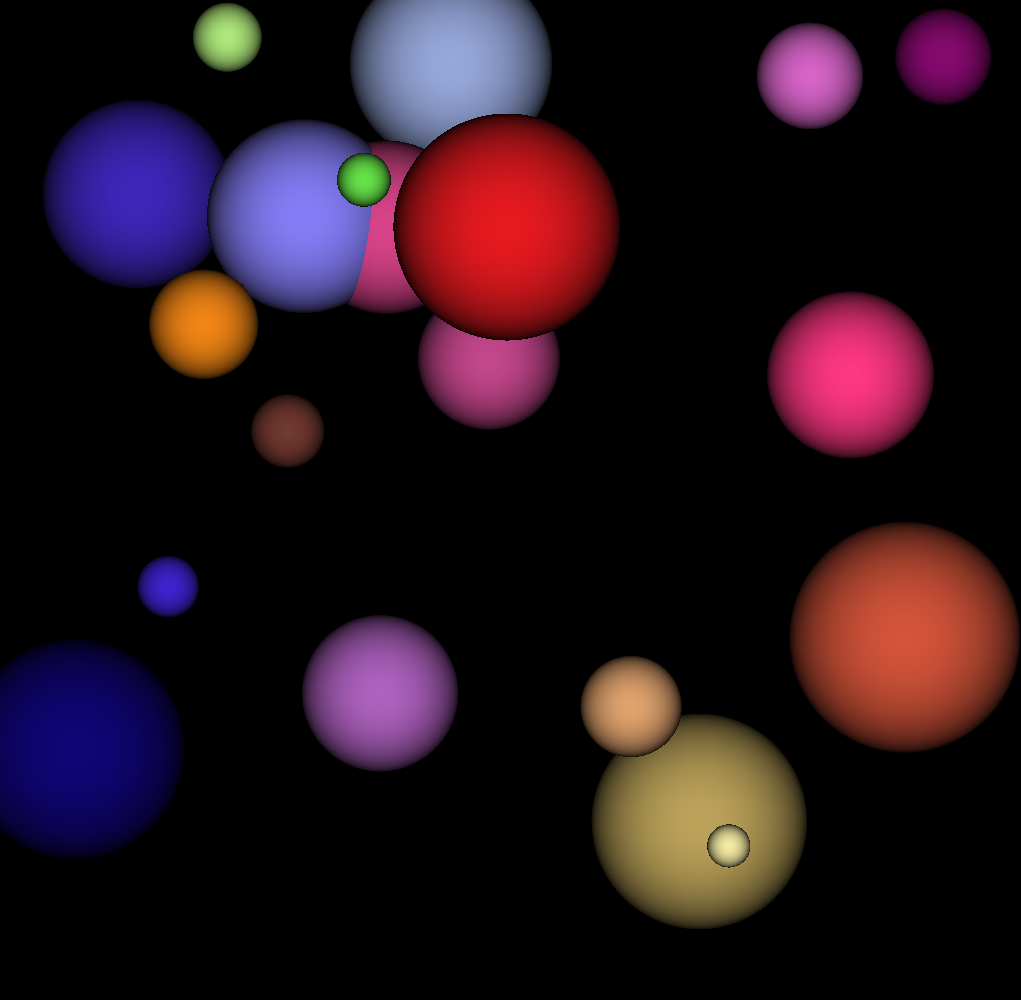
\includegraphics{RayTracing.png}
\caption{A screenshot from the ray tracing example}\end{figure}


\subsection{Performance}
\label{RTACM/RTACM:performance}\begin{description}
\item[{We conducted 5 tests and the results are below.}] \leavevmode\begin{itemize}
\item {} \begin{enumerate}
\item {} 
6.7 ms

\end{enumerate}

\item {} \begin{enumerate}
\setcounter{enumi}{1}
\item {} 
6.8 ms

\end{enumerate}

\item {} \begin{enumerate}
\setcounter{enumi}{2}
\item {} 
6.8 ms

\end{enumerate}

\item {} \begin{enumerate}
\setcounter{enumi}{3}
\item {} 
6.7 ms

\end{enumerate}

\item {} \begin{enumerate}
\setcounter{enumi}{4}
\item {} 
6.8 ms

\end{enumerate}

\item {} 
Average: 6.76 ms

\end{itemize}

\end{description}


\section{Constant Memory}
\label{RTACM/RTACM:constant-memory}
We have mentioned that there are several types of memory in CUDA architecture. Till now, we have seen global memory and shared memory. This time, we will explore the characteristics of constant memory.

By its name, constant memory is designed to store variables that will not change when the kernel is executing commands. Constant memory is located in global memory, which means constant variables are stored in the global memory as well. However, constant variables are cached for higher access efficiency. Just like shared memory, there is always price come with faster access speed. The CUDA architecture provides only 64KB of space for global memory. Therefore, constant memory is not designed to store large dataset.


\section{Ray Tracing With Constant Memory}
\label{RTACM/RTACM:ray-tracing-with-constant-memory}
In the example of ray tracing, we will see how to improve program efficiency by using constant memory. We do this by store 20 sphere object in the constant memory for faster access. In our example, every pixel of the image needs to access 20 sphere objects over the course of kernel execution. If we have a bitmap of the size \emph{1024x1024}, we are looking at over one million times of access for each of the sphere.

Ray Tracing With Constant Memory source file:
\code{ray.cu}


\subsection{Constant Memory Declaration}
\label{RTACM/RTACM:constant-memory-declaration}
\begin{Verbatim}[commandchars=\\\{\}]
\PYG{n}{\PYGZus{}\PYGZus{}constant\PYGZus{}\PYGZus{}} \PYG{n}{Sphere} \PYG{n}{s}\PYG{p}{[}\PYG{n}{SPHERES}\PYG{p}{]}\PYG{p}{;} \PYG{c+c1}{// declare spheres in constant memory}
\end{Verbatim}

This line of code shows you how to declare variables in constant memory. The only difference is that you have to add \textbf{\_\_constant\_\_} qualifier before the declaration.


\subsection{Structure \& Device Code}
\label{RTACM/RTACM:structure-device-code}
The device code and the code to create structure are exactly the same as the version not using constant memory.


\subsection{Host Code}
\label{RTACM/RTACM:id1}
Most of the host code is the same as the version not using constant memory. There are only two different places. First, since we have already prepared spaces in constant memory for Sphere dataset, we do not use the command \emph{cudaMalloc()} and \emph{cudaMemcpy()} anymore to allocate it in global memory anymore. Second, we use the following code to copy initialized Sphere dataset to the constant memory.

\begin{Verbatim}[commandchars=\\\{\}]
    \PYG{c+c1}{// transfer the initialized Sphere dataset to constant memory}
    \PYG{n}{HANDLE\PYGZus{}ERROR}\PYG{p}{(} \PYG{n}{cudaMemcpyToSymbol}\PYG{p}{(} \PYG{n}{s}\PYG{p}{,} \PYG{n}{temp\PYGZus{}s}\PYG{p}{,} 
                                \PYG{k}{sizeof}\PYG{p}{(}\PYG{n}{Sphere}\PYG{p}{)} \PYG{o}{*} \PYG{n}{SPHERES}\PYG{p}{)} \PYG{p}{)}\PYG{p}{;}
\end{Verbatim}


\subsection{Performance}
\label{RTACM/RTACM:id2}\begin{description}
\item[{We conducted 5 tests and the results are below.}] \leavevmode\begin{itemize}
\item {} \begin{enumerate}
\item {} 
6.2 ms

\end{enumerate}

\item {} \begin{enumerate}
\setcounter{enumi}{1}
\item {} 
6.1 ms

\end{enumerate}

\item {} \begin{enumerate}
\setcounter{enumi}{2}
\item {} 
6.3 ms

\end{enumerate}

\item {} \begin{enumerate}
\setcounter{enumi}{3}
\item {} 
6.4 ms

\end{enumerate}

\item {} \begin{enumerate}
\setcounter{enumi}{4}
\item {} 
6.4 ms

\end{enumerate}

\item {} 
Average: 6.28 ms

\end{itemize}

\end{description}

Due to the small bitmap size we are using, the improvement is not significant.



\renewcommand{\indexname}{Index}
\printindex
\end{document}
